%\document class[]{aiaa-tc} %load in aiaa class template file
\documentclass{article}
\usepackage{amsmath}
\usepackage{mathrsfs}
\usepackage{enumitem}
\usepackage{mathabx}
\usepackage{hyperref}
\usepackage{natbib} %REMOVE THIS IF YOU DON'T WANT BRACKETS ON YOUR PAPER
\usepackage{float}
\usepackage{color,soul}
\usepackage[font=normalsize,labelfont=bf]{caption}
\usepackage[left=2cm,right=2cm,top=2cm,bottom=2cm]{geometry}
\usepackage{graphicx}
\usepackage{hyperref}
\usepackage{xcolor}

\newcommand{\sref}[1]{$^{[\ref{#1}]}$}
\newcommand{\dref}[2]{$^{[\ref{#1}-\ref{#2}]}$}

 % Define commands to assure consistent treatment throughout document
\newcommand{\eqnref}[1]{(\ref{#1})}
\newcommand{\class}[1]{\texttt{#1}}
\newcommand{\package}[1]{\texttt{#1}}
\newcommand{\file}[1]{\texttt{#1}}
\newcommand{\BibTeX}{\textsc{Bib}\TeX}
%\newcommand{\href}[1]{\href{#1}{

\hypersetup{%
  colorlinks=true,% hyperlinks will be black
  linkcolor=blue,
  linkbordercolor=red,% hyperlink borders will be red
   %pdfborderstyle={/S/U/W 1}% border style will be underline of width 1pt
}

\makeatletter
\Hy@AtBeginDocument{%
  \def\@pdfborder{0 0 1}% Overrides border definition set with colorlinks=true
  \def\@pdfborderstyle{/S/U/W 1}% Overrides border style set with colorlinks=true
                                % Hyperlink border style will be underline of width 1pt
}
\makeatother

\begin{document}

\title{Project Based Engineering Instrumentation With CircuitPython}
\author{Carlos Montalvo\footnote{Montalvo: William B. Burnsed Jr. Department of Mechanical, Aerospace and Biomedical Engineering, Associate Professor}
  \\University of South Alabama\\Mobile, AL\ \\ \ \\Marine Feron Leabeater \footnote{Leabeater: Lounsbury College of Education, EdD Graduate Student}\\Georgia College and State University \\ Milledgeville, GA\ \\ \ \\Lisa Schibelius\footnote{Schibelius: Department of Engineering Education, PhD Graduate Research Assistant}\\
Virginia Polytechnic Institute and State University\\Blacksburg, VA}

\maketitle

\linespread{1}

\newpage

\section*{Current Edition}

This manuscript was last updated on \today. 
The latest edition can be found on \href{https://github.com/cmontalvo251/LaTeX/blob/master/PBL_CircuitPython_Instrumentation/main.pdf}{Github}

\section*{Manuscript Changes}

\begin{enumerate}[itemsep=-5pt]
\item Original tutorials in Google Docs created
\item December 21st, 2021 - Updated links for manuscript and hardware
\item Tutorials purchased by \href{https://tangibles-that-teach.gitbook.io/instrumentation-lab-manual/-MbMx70LQzRmEG_hS7Ld/}{Tangibles that Teach}
\item May 30th, 2022 - Tangibles that teach went out of business and
  chapter began the move to Github
\item June 28th, 2022 - Work began on a Chromebook. Unfortunately the
  Figures folder is not back up on Git. As such a main\_latest.pdf has
  been created that's the latest full version. The main.pdf is the
  version created by the Chromebook so it has new chapters but none of
  the older chapters. Figure files are now backup on Git but only
  figures from the 'Voltage Potentiometer' are currently there.
\item July 2nd, 2022 - All figures backed up and latest manuscript completed
\item October 18th, 2022 - A pedometer lab has been added.
\item November 8th, 2022 - Edited the Servo and feedback control servo
  lab to be one big lab with 3 parts
\item January 8th, 2023 - Removed all mentions of Tangibles that Teach
  in the main body of the text.
\item February 6th, 2023 - Changed an assignment description for LEDs
  and push buttons
\item February 22nd, 2023 - Moved the Bluetooth module to be before
  the modules lab so this will end up being a few updates to make
  those projects more uniform. I also created a backup called
  Bluetooth original in case you wanted to go back to the other version.
\item June 16th, 2023 - Cleaned up the ``changes needed" list and updated Method 3 with some new software updates.
\item August 9th, 2023 - Edited the preamble for assignments and made a note in the servo lab
\item September 5th, 2023 - Updated hyperlinks to show up on Microsoft Edge using underlines and different color text.
\item September 7th, 2023 - Fixed the TL;DR section
\item September 15th, 2023 - Updated a link in the DAQ lab
\item September 20th, 2023 - Made the modules installation section a standalone tex file
\item October 4th, 2023 - Added a new potentiometer photo
\item November 16th, 2023 - Edited the lists of parts 
\item November 22nd, 2023 - Edited acceleration lab
\item December 5th, 2023 - Edited the troubleshooting section
\item January 12th, 2024 - Edited chapters 1 and 2
\item January 22nd, 2024 - Edited the bootloader update notes in the troubleshooting chatper
\item January 25th, 2024 - More edits to the bootloader notes
\item March 20th, 2024 - Added a preamble about where this textbook is located
\item April 27th, 2024 - Previously edited servo lab and pendulum lab just the assignment portion and then added this change log to the manuscript
\item May 7th, 2024 - Title page changed and many sections moved around. Added a new results and discussion section following data analysis from course surveys of this course.
\item August 12th, 2024 - Added a new requirement for the servo lab
\item September 12th, 2024 - A few edits to assignment descriptions
\item October 25th, 2024 - Updated the photocell lab to include the number of data points for the histogram
\item November 11th, 2024 - Updated Method 3 quick list 
\end{enumerate}

\newpage

\tableofcontents

\newpage

\newpage

\section{Introduction}

This textbook describes an instrumentation kit used for an
Instrumentation and Experimental Methods course at the undergraduate
level. This textbook has been designed with the student and faculty member in
mind. The kit contains the CircuitPlayground
Express/Bluefruit running CircuitPython and is used to teach
fundamentals of instrumentation and provide a hands-on way of
learning. Engineering is usually taught in a
traditional lecture format, involving theory in the classroom,
homework outside of class, and routine examinations. Progressive forms
of learning such as flipped classrooms and project based learning
(PBL) have created new and fun ways for professors to interact with
students and for students to be more involved in their learning. PBL
provides a student-centered method of teaching and learning by posing
problems for students to solve with the solution of the project being
the primary goal and the theory a secondary goal.

The course begins with simple plotting and moves into data analysis,
calibration and more complex instrumentation techniques 
such as active filtering and aliasing. This course is designed to get
students away from their pen and paper and build something that blinks
and moves as well as learn to process real data that they themselves
acquire. There is no theory in these projects. It is all applied using
the project based learning method. Students will be tasked with
downloading code, building circuitry, taking data all from the ground
up. By the end of this course students will be well versed in the
desktop version of Python while also the variant CircuitPython
designed specifically for microelectronics from Adafruit. After this
course students will be able to understand Instrumentation at the
fundamental level as well as generate code that can be used in future
projects and research to take and analyze data. Python is such a broad
and useful language that it will be very beneficial for any
undergraduate student to learn this language. To the professors using
this textbook, 1 credit hour labs are often hard to work into a
curriculum and “live” demonstrations in the classroom cost time and
money that take away from other faculty duties. I’ve created this kit
and textbook to be completely stand-alone. Students simply need to
purchase the required materials and follow along with the
lessons. These lessons can be picked apart and taught sequentially or
individually on a schedule suited to the learning speed of the
course. The authors hope that whomever reads and learns from this
textbook will walk away with an excitement to tinker, code and build
future projects using microelectronics and programming. The
implementation of this kit and overall teaching method has received
many positive reviews from students and is reflected in anonymous course
evaluations.

Students can learn in many ways with a variety of different
omodalities \cite{Gardner}. As such, instructors can choose how to
present course material and have students develop content-specific
skill sets. College students enter the classroom with existing skills
in multi-disciplinary learning that is practiced at the secondary
school level \cite{Ralph}. College and university professors have
the opportunity to use these existing skills as a foundation for their
own instructional practices. Traditional lectures provide students
with lectures on theory. The instructor then provides examinations to
the students based on that theory. Using this format, an instructor
can focus on mathematical principles, the so-called building blocks of
engineering or provide specific applications to these
models \cite{Learning_Styles}. In a traditional lecture format,
the instructor presents theory to the students with academic problems
rarely encountered in a students future career, building invaluable
theoretical knowledge of concepts that appear disconnected from
practical knowledge applied in the field \cite{Yong}. Historically
in engineering education, there has been tension between theory and
application \cite{PBL1}.  Applications include case studies or
practical engineering problems that emulate future careers in
engineering. This provides students with engineering phenomena that
they can see and hear. They can reason through problems intuitively,
memorize facts using demos, build mathematical models, or build
tangible objects themselves. With these different presentation
methods, students are exposed to engineering phenomena in multiple
ways rather than just on the
whiteboard\cite{Learning_Styles}. Project Based Learning (PBL)
provides an alternative for conventional teaching by facilitating
problem solving for students in a group setting that requires
communication, critical thinking, and creativity. These types of
problems have shown that heightened learning can happen when students
interact with tangible objects that represent the theory they are
presented with in the classroom \cite{PBL_Book}. Rather than
learning an equation for heat transfer along a one-dimensional pipe,
the students can create a pipe with thermocouples and plot data from
multiple sensors along the pipe. This connection to a tangible object
reinforces learning and allows students to form bridges in
comprehension between their theoretical knowledge and practical
application (practical knowledge) of those theories in the
field\cite{TANGIBLEINTERFACES}. Research has shown that a
classroom that creates an integrated curriculum increases student
satisfaction which immediately correlates to satisfactory student
performance and increased graduation
rates \cite{StudentSatisfaction}. This is an example of the
benefits of active student engagement versus passive student
engagement. While the traditional lecture format is vital to students
understandings, it is understood that application of the concepts
covered in lecture are  
required to reach higher levels of learning \cite{Armstrong}.  

%\subsection{Background}
%This should include summary of prior work
Hands-on projects where students interact with tangible objects is not
a new form of teaching. The laboratory environment has been around for
decades. However, typically the classroom environment is separate from
the laboratory environment.  There has been little synergy between the
two learning environments. A Mechanical Engineering degree is likely
to have around three to four labs in various disciplines. In these
courses, students perform an experiment in groups. They take and
analyze data as well as create a report documenting their
findings. Many of these laboratory experiments of course are
choreographed for the student by the instructor. They follow a script
and perform the experiment without building anything themselves. The
students take no ownership over the experiment and there is no
creativity built-in. Over the years, the nature of laboratories has
changed including the lack of clear learning
objectives \cite{Labs}. Furthermore, this laboratory environment
requires a significant amount of instrumentation and hardware to
implement. For example, a shock tube or steam pump can cost tens of
thousands of dollars. The maintenance and up-keep alone is not
practical for smaller institutions. The teaching investment required
to prepare the lab every year and the lab itself (often on the order
of three hours) can be a time consuming task for a tenure track
faculty member who often has a large research load. 

The so-called "Lab at Home" hardware kits are becoming more and more
common in the classroom to ease the burden on the instructor and
institution itself\cite{LabAtHome}. These kits are small enough to be
purchased and shipped to a student for them to perform experiments
remotely rather than in the classroom itself\cite{LabAtHome1}. They
can also be brought to the classroom to be used as a personal demo
aid\cite{LabAtHome2_EE}. In this sense, the take-home lab kit serves
as a bridge between theory based lectures and a laboratory
setting\cite{LabAtHome3}. This allows both instructors and students to
engage with content in a way that promotes enduring understandings and
practical application of theoretical
knowledge\cite{LabAtHome4_EE}. Since the kits can be used remotely,
they can also be used for distance learning courses or other
asynchronous activities as well as during the COVID-19 pandemic.   

Two home kits in particular are directly related to instrumentation
and circuits. Cyganski and Nicoletti\cite{LabAtHome4_EE} for example
created a new curriculum for first year electrical engineering
students by creating live demonstrations for the students. Manijikian
and Simmons\cite{LabAtHome2_EE} however, combined a popular commercial
microcomputer board with their own custom-designed interface board in
a kit that students retain for the duration of the course for both
in-lab and at-home assignments. The take-home kits however were based
on the Motorola 68HC11EVB microcomputer which is programmed in
assembly language. Assembly language is a rather difficult language to
learn at the undergraduate level. Even with such a difficult learning
curve, however, student feedback on their approach was
positive\cite{LabAtHome2_EE}. 

It is clear that using a lab at home kit is useful for the
instrumentation classroom, however the programming language to be used
is a subject of debate in faculty meetings and computing
committees. There are multiple languages in use today of varying
complexities and use cases. There are scripting languages like Python,
Ruby and MATLAB, object oriented languages like Java and C++ and
compilation languages like Fortran and C. Note, this is not an
exhaustive list. A recent study showed that scripting languages
(Python, Ruby, MATLAB) enable writing more concise code while
compilation languages (C, Fortran) create smaller
executables \cite{codetype}. MATLAB is often considered in engineering
given its success in industry and its ability to perform numerical
simulations and plotting with ease. Python, however, has become more
and more popular with numerical toolboxes like numpy and plotting
toolboxes like matplotlib that are free and easy to install in
integrated development environments like Thonny or
Spyder \cite{IDE}. The Tiobe Index of Programming\cite{Tiobe} has the
top 3 programming languages listed as Python, C, and Java. MATLAB
is \#20 on the list. In 2004, Hans Fangohr wrote that MATLAB is much
better suited than C for engineering computing but the best choice in
terms of clarity and functionality is provided by
Python \cite{CodeComparison}. It seems then that it would be more
practical for educators even in engineering to teach the most popular
language. This helps with transferability of skills and has future
implications for a students' career. The scripting aspect of Python
lowers complexity and allows students to learn the language quickly to
apply it as a tool rather than getting stuck memorizing syntax and
compilation rules. The language also comes at no cost to the
students. This is a plus for students already bearing heavy financial
burdens to attend a university which includes tuition and
institutional fees. 

Given the success of other kits in many classes and the popularity of
Python, the University of South Alabama (USA) has implemented such a
kit for Instrumentation \& Experimental Methods (ME 316) using
CircuitPython. CircuitPython is a derivative of Python written for
embedded systems and designed to simplify experimenting and learning
to code \cite{CircuitPython}. The learning objectives for ME316
include: statistics, dynamic response of measurement systems,
operational amplifiers, signal conditioners and fundamentals of
microprocessors. This course could be taught with theory as the main
focus of the lecture. However, this course includes the use of an
instrumentation kit and Project Based Learning methods in addition to
theory in the classroom. Each student taking the course purchases the
kit and downloads a free accompanying project
list \cite{Gitbook}. Every Friday, the students complete one of the 20
projects. The following week they submit a report which includes a
demo of the working project in the form of photos and videos, any
plots generated if they are required to take data, all code used and a
small write-up explaining their findings. The sections that follow
describe the kit in more detail as well as student evaluations who
have taken the course.

Note that, the Adafruit Learn page contains many tutorials on how to operate the
CircuitPlayground\cite{Adafruit}. However, Adafruit sells much
more than just the CPX and thus it is often difficult for anyone to
find the correct tutorial needed for the CPX. A simple search on the
Adafruit Learn System yields 21 results for "servo" just on the first
page with over 48 pages of results. The tutorial needed to run a servo
with CircuitPython is the 10th result and it's for a different
development board. Although the software works with the CPX, it does
not explicitly say so. Due to the complexity of some of these systems,
documentation was made and freely given to the
community\cite{Gitbook}. This documentation was custom built using a
combination of multiple sources across the internet. All software for
the kit is also
on \href{www.github.com/cmontalvo251/Microcontrollers.git}{Github} in
a separate repository. Each chapter in the book contains one project for the
students to complete on their own. A list of chapters and a brief
description of the assignment is shown in the table of
contents. Currently there are 20+ projects for the students to work on.

\section{Course Description}

The course is designed to coincide with lecture content in a standard
engineering instrumentation course. The students are guided through
numerous projects. The specific course learning objectives, which include
statistics, dynamic responses, operational amplifiers, and electronic
circuits both analog and digital are shown below:
\begin{enumerate}[itemsep=-5pt]
\item Apply statistical concepts of error and uncertainty analysis using normal,“t” distribution and the $\chi^2$ distribution
\item Use propagation of error methods to determine the uncertainty of calculated quantities
\item Apply the concepts of harmonic response to predict the response of measuring systems to input signals
\item Apply the fundamentals of operational amplifiers and electronic circuits to design signal conditioning circuits including %amplification and filtering
\item Apply microprocessor fundamentals to gain an understanding of digital circuits used for digital to analog and analog to digital conversion
\end{enumerate}

This course is not going to be a traditional lecture format and that
hands-on projects will be assigned every Friday using the lab at home
kit. The projects every Friday are created to enhance the course
learning objectives as dictated above.  

The course is taught on a 2+1 style where the course meets three days
a week for 50 minutes each on Monday, Wednesday and Friday. On Monday
and Wednesday the class is similar to what would typically be found in
a standard lecture format. The instructor goes through theory and examples on a
white board. On Fridays, the students come to class with their
hardware kits and laptops to perform one of 20+ projects defined in
the tutorials in this textbook. Fridays are nicknamed "Funday Fridays"
to differentiate the format of the class and to get students excited about the
projects. On Fridays, the instructor can walk around the classroom and
assist students on their projects as well as highlight fundamental
concepts. This is done by showing them what they learned on a
whiteboard with their lab at home kit. During the COVID-19 pandemic
when Universities were meeting via Zoom, class time on Friday was used
to assist students on their projects while they showed their circuits via
webcam in a virtual space. Since all students purchased their own kit,
there was no issue with students getting hands-on experience even
during COVID-19.  

It is important to note here that Project Based Learning (PBL) in this
course did not replace existing teaching frameworks; rather, PBL
supplemented existing standard teaching measures by allowing students
to apply theory to practice. The role of connectivism comes from the
online networking tools that were added to the curriculum. The
tutorials and assignments as well as example code are all hosted
online on Github \cite{Github}. The availability of these
tutorials and software opens the students to an ecosystem of free and
open source software. Furthermore, the Adafruit Learning System is
also used occasionally which opens them to an ecosystem of hardware
and software tutorials as well as Adafruit IO (an internet of things
site) and the Adafruit Forums \cite{Adafruit}. The Adafruit Forums
allow the students to comment and communicate with other groups
outside the university that utilize the same hardware kits. If the
instructor cannot find a solution online in a Wiki or Tutorial page, a
student or the instructor can post on the forum and wait for a
response from the larger Adafruit community. 

Students in this course are also required to do a final project
where they must create something new by using the microcontroller in
the kit plus three other electrical components. One of the three
components must be something not originally included in the kit. The
students may also work in a group. PBL typically consists of
ownership, creativity, collaboration and critical thinking. These four
aspects are clearly a big part of this lab at home kit and the final
project. They can work in groups: collaboration. They must make
something new: creativity. They must build the item themselves:
ownership. They must apply fundamental principles of the course:
critical thinking. In addition to PBL aspects, the students are
exposed to the larger network of learning through Github, the Adafruit
Learning system and Forums as well as general Wikis online. This
network of learning is seen in the connectivism framework.





\newpage

\newpage

\section{Purchase Equipment}

\subsection{Items needed for this Lab}

\begin{enumerate}[itemsep=-5pt]
\item Laptop with internet connectivity
\item Credit/Debit Card to Purchase items
\end{enumerate}

\subsection{CircuitPython Kit}

In this class you’re going to build some circuits that will enhance
your learning experience. Rather than just solving problems by hand
you’re going to take and analyze data. Over the summer of 2020, I
began to work with Tangibles that Teach and at the time they bundled
all components together. Unfortunately, that company has gone out of
business and as such for the time being you must build the kit
yourself. Here is a list of all the components in the kit

\begin{enumerate}[itemsep=-5pt]
\item Circuit Playground Bluefruit or Express + Included USB Cable
\item Micro Servo
\item Potentiometer
\item Photocell
\item Two Resistors (330 Ohm and 1K Ohm)
\item Alligator Clips x3
\item External Battery Pack
\item AAA Batteries x3
\item Breadboard
\item Push Button 
\item LEDs x2
\item Pitot Probe
\item LSM6DS33 + LIS3MDL - 9 DoF IMU (Optional)
\end{enumerate}

Below is also a photo of all the components listed above. When you get
your kit familiarize yourself with all of the components. I created
an \href{https://youtu.be/6sNNQrhnzLE}{unboxing video on Youtube} 
for you to take a look. The hardware kit is a collection of multiple
items. At the time of this writing the entire kit cannot be purchased
however the CircuitPlayground Express (CPX) can be purchased on
Adafruit\cite{AdafruitMAIN}. A photo of the kit is shown in the figure below. The photo shows the CPX on the left inside it's
protective zip lock bag.

\begin{figure}[H]
  \begin{center}
    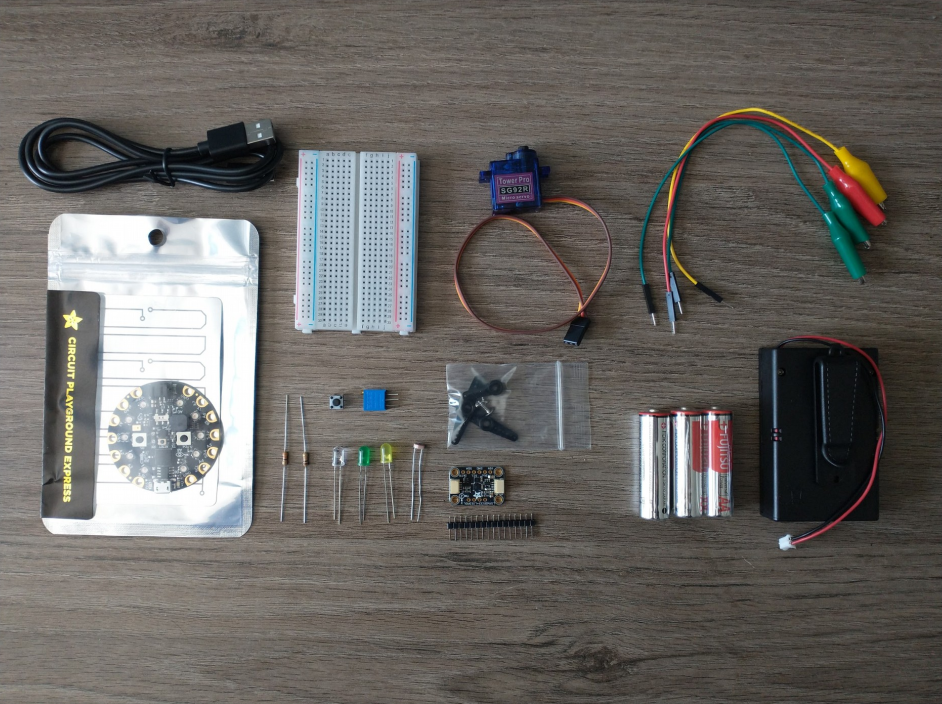
\includegraphics[width=0.8\textwidth]{Figures/components.png}
  \end{center}
\end{figure}

The CPX is a relatively new development board that operates in the
same style as Arduino\cite{Arduino}. That is, the student can
create a relatively simple script and then flash the software to the
CPX via USB. The Arduino operates in the same way. The benefit of the
CPX vs the Arduino is that the software is CircuitPython which is
indistinguishable from Python. As mentioned earlier, Python is in the
top 3 programming languages as stated by the Tiobe Index of
Programming\cite{Tiobe}. Other benefits include the components
built in to the CPX. The CPX itself contains a built in microphone,
accelerometer, light sensor, speaker, three push buttons, slide switch
and infrared sensor. The CircuitPlayground Express (CPX) also contains
10 smart NeoPixel LEDs and a ring of copper plated pads that can be
attached to the included alligator clips and breadboard. Students can
also elect to purchase the CircuitPlayground Bluefruit (CPB) which
does not have an infrared sensor but does contain bluetooth
functionality to send data wirelessly to the Adafruit Connect App
which runs on Apple/Android\cite{AdafruitBLE}.

\subsection{Assignment}
Your assignment for this module is to purchase the required equipment for your class. Note that the specific equipment will be instructor dependent so be sure you discuss with the instructor of your course before buying everything. At a minimum you must purchase a CPX or CPB but the rest of the items in your kit will depend on which modules your instructor wants you to do during the semester. {\bf Note that the CPX/CPB requires a microUSB cable and that cable must have a data line. Many USB cables are just power and ground.}

Once you've completed the project above, upload a PDF with all of the photos and text
below included. My recommendation is for you to create a Word document
and insert all the photos and text into the document. Then export the
Word document to a PDF. For videos I suggest uploading the videos to
Google Drive, turn on link sharing and include a link in your
PDF. Note that all code must be included in the appendix or you'll be
penalized 10\%. 


\begin{enumerate}[itemsep=-5pt]
\item A figure of your receipt of your purchases this semester - 80\%
\end{enumerate}

%\subsection{Quick Links}
%\begin{enumerate}[itemsep=-5pt]
%  \item \href{https://www.tangiblesthatteach.com/product-page/instrumentation-kit-for-me-316}{Kit}
%  \item \href{https://a2279211-28c1-4f46-9477-0d3265900c7f.filesusr.com/ugd/2413aa_ca39175b0a514b838ec96893b90590eb.pdf}{Document}
%  \item \href{https://youtu.be/6sNNQrhnzLE}{Unboxing Video}
%\end{enumerate}
%\subsection{Turning in this assignment}
%\begin{enumerate}[itemsep=-5pt]
%  \item Upload a receipt of ALL of your purchases - 50\%
%  \item Put your name and the names of your group members. If working
%    alone, tell me you are planning on working alone in the PDF you
%    upload. In times of COVID, everyone is working alone - 50\%
%\end{enumerate}
%% \newpage

%% \begin{center}\LARGE{ONLY READ BELOW IF YOU DON’T WANT TO BUY THE KIT
%%     ABOVE}\end{center}

%% \subsection{Purchase Items Yourself}

%% The bill of materials listed below is designed for 2 or 4 students to work together and share
%% pieces. This kit is not optimized for 3 students. If you are a remote/online student or you just
%% prefer to work alone then you have the option of purchasing everything yourself. The cost per
%% student in a group of 4 and 2 is listed as well as the cost if working alone. You’ll find that even
%% with the optional equipment, the cost of working alone is still less than the price of a standard
%% college textbook. Note that if you are working alone, be sure to only purchase 1 of each item. If
%% working in pairs you also have the option of purchasing one of each item. Finally, if you own
%% some of these components you may wish to simply purchase each item separately. A detailed
%% parts breakdown is shown after the rubric.

%% \subsection{Bill of Materials (per 4 students)}

%% \begin{figure}[H]
%%   \begin{center}
%%     \begin{tabular}{|l|c|c|}
%%       \hline
%%       Item (ONLY IF YOU DON’T WANT THE KIT ABOVE) & Quantity & Total
%%       Cost \\
%%       \hline
%%       \href{https://www.adafruit.com/product/3333}{Circuit Playground Express (CPX)} & 2 & \$50 \\
%%       \hline
%%       \href{https://www.adafruit.com/product/169}{Servo} & 2 & \$10 \\
%%       \hline
%%       \href{https://www.adafruit.com/product/592}{USB Cable} & 2 & \$6 \\
%%       \hline
%%       \href{https://www.amazon.com/Smraza-Breadboard-Resistors-Mega2560-Raspberry/dp/B01HRR7EBG/ref=sr_1_3?dchild=1&keywords=photocell+circuit+kit&qid=1590531716&sr=8-3}{Electronics Kit} (Photocells, Resistors, Trimpot) & 1 & \$13 \\
%%       \hline
%%       \href{https://www.amazon.com/WGGE-WG-026-Pieces-Colors-Alligator/dp/B06XX25HFX/ref=sr_1_1_sspa?dchild=1&keywords=alligator+clips&qid=1613147431&sr=8-1-spons&psc=1&spLa=ZW5jcnlwdGVkUXVhbGlmaWVyPUFLRjlYRVM3SDIySVAmZW5jcnlwdGVkSWQ9QTAwNDczMzEyODNCVTJWSjlMR0NEJmVuY3J5cHRlZEFkSWQ9QTAwMDQyMjkzSlJLNjJRWk9CSVZEJndpZGdldE5hbWU9c3BfYXRmJmFjdGlvbj1jbGlja1JlZGlyZWN0JmRvTm90TG9nQ2xpY2s9dHJ1ZQ==}{Alligator Clips} & 1 & \$4 \\
%%       \hline
%%       {\bf Total} & & {\bf \$83} \\
%%       \hline
%%       {\bf Cost per student in a group of 4} & & {\bf \$21} \\
%%       \hline
%%       {\bf Cost per student in a group of 2} & & {\bf \$25} \\
%%       \hline
%%       {\bf Cost if working alone} & & {\bf \$50} \\
%%       \hline
%%        & & \\
%%       \hline
%%       {\bf Optional Equipment} & & \\
%%       \hline
%%       \href{https://www.adafruit.com/product/3287}{External Power Supply} & 2 & \$6 \\
%%       \hline
%%       \href{https://www.adafruit.com/product/3349}{AA Batteries} & 2 & \$6 \\
%%       \hline
%%       \href{https://www.amazon.com/Hobbypower-Airspeed-MPXV7002DP-Differential-controller/dp/B00WSFWO36/ref=sr_1_3?dchild=1&keywords=Airspeed+sensor+kit&qid=1590532161&sr=8-3}{Analog Pitot Probe} & 1 & \$31 \\
%%       \hline
%%       \href{https://www.adafruit.com/product/4485}{Rate Gyro (LSM6D3SS)} & 1 & \$10 \\
%%       \hline
%%       & & \\
%%       \hline
%%       {\bf Total with Optional Equipment} & & {\bf \$136} \\
%%       \hline
%%       {\bf Cost per student in a group of 4} & & {\bf \$34} \\
%%       \hline
%%       {\bf Cost per student in a group of 2} & & {\bf \$50} \\
%%       \hline
%%       {\bf Cost if working alone} & & {\bf \$97} \\
%%       \hline
%%     \end{tabular}
%%   \end{center}
%% \end{figure}

%% \subsection{Detailed Parts List}

%% If you want to just purchase each component separately you can, just
%% make sure you have all of the parts below.

%% \begin{enumerate}[itemsep=-5pt]
%%   \item Circuit Playground Express (CPX)
%%   \item Servo
%%   \item Alligator Clips
%%   \item USB Cable
%%   \item Push Button
%%   \item Breadboard
%%   \item Photocell
%%   \item Resistors (10 kOhm, 330 Ohm, 1 kOhm)
%%   \item LED (x3 in case you fry one)
%%   \item Male to Male Wires (x2)
%%   \item Potentiometer
%% \end{enumerate}

%% You can also purchase some optional equipment as shown below.

%% \begin{enumerate}[itemsep=-5pt]
%% \item Rate Gyro (LSM6D3SS)
%% \item Male to Male Wires (x2)
%% \item Alligator Clips (x1)
%% \item Double Sided Tape
%% \item Analog Pitot Probe
%% \end{enumerate}

\newpage 

\section{Download Python for Desktop}

As you learn Instrumentation throughout the semester, you will be
tasked with creating computer programs on the Circuit Playground
Express (CPX). The CPX itself has it’s own RAM, CPU, HDD and many
sensors. Your CPX is kind of like a mini computer! You can plug the
CPX into your computer via USB and access the hard drive (HDD) from
your own computer. When you program on the CPX you need to write
programs on the CPX itself so that the mini computer can run the
program you wrote. The CPX knows how to read multiple different
languages but in this class we are going to write everything in the
\href{https://www.python.org/}{Python} language which has been ported
to the CPX and called
\href{https://circuitpython.org/}{CircuitPython}. Since we have to
write everything in CircuitPython we 
need to first learn how to program some things in Python. You can
easily download Python by itself but it’s nice to get what’s called an
Integrated Development Environment (IDE). This way you can practice
writing Python code on your computer while you wait for your purchases
to arrive in the mail. 

So which IDE can you download and which is recommended? I recommend
two IDEs. They are listed below. I recommend getting either one. If
you just Google “Python download” you will find a humongous list of
editors (Scratch, Anaconda, Canopy, Eclipse, PyDev, etc). It’s easy to
get lost when searching for something so broad. You’ve been warned.

\subsection{Thonny}

Thonny - \url{https://thonny.org/} -
\href{https://www.youtube.com/watch?v=qaxukpYRqfA&list=PL_D7_GvGz-v1RsDs_OdNW65qRjEjmpfQx&index=14}{Youtube
  video on how to install}

\begin{figure}[H]
  \begin{center}
    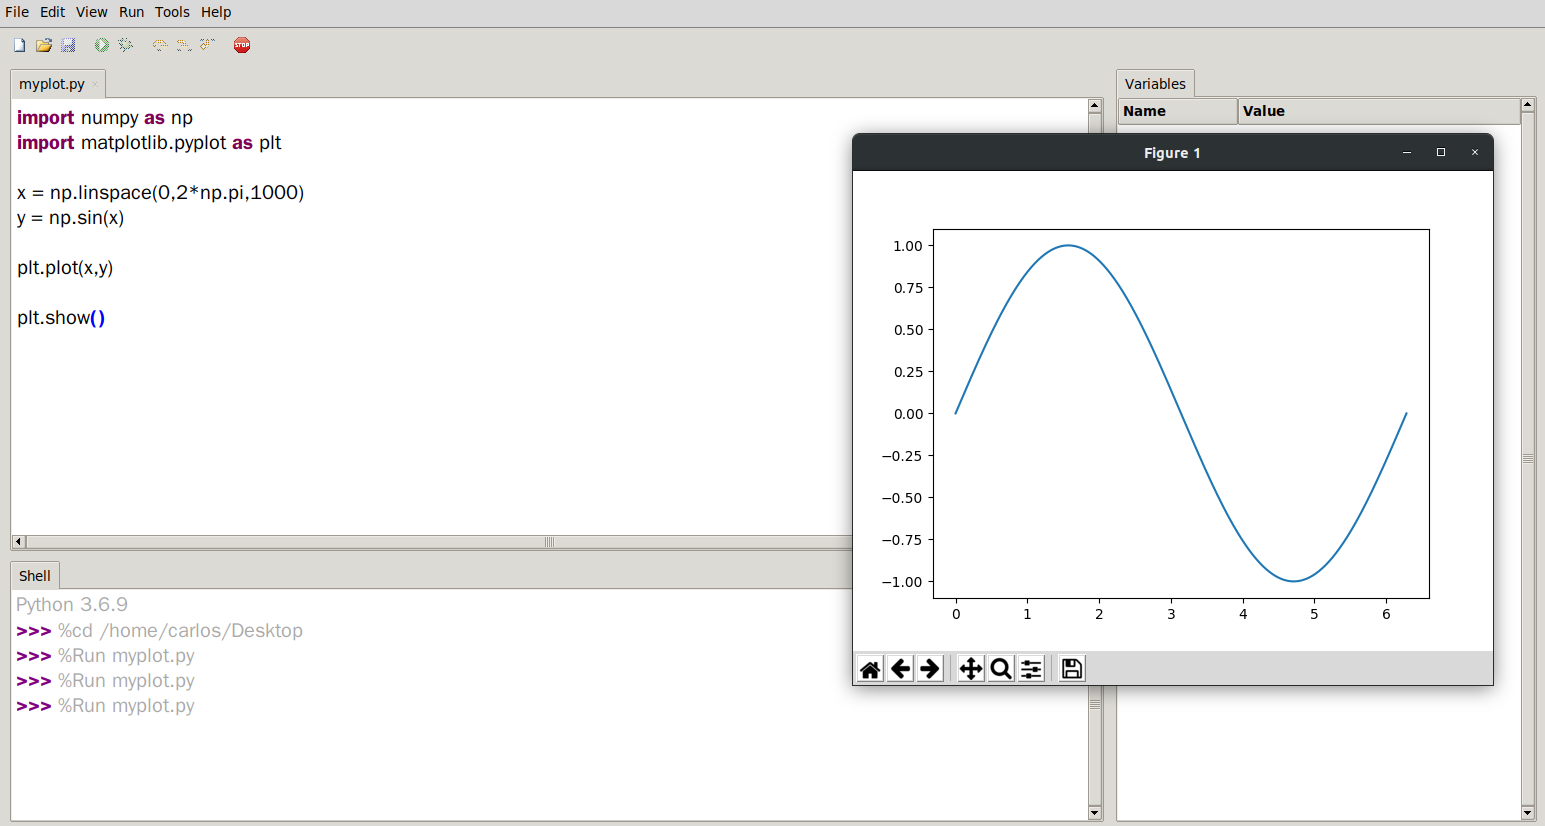
\includegraphics[width=\textwidth]{Figures/Thonny.png}
  \end{center}
\end{figure}

\subsection{Spyder}

Spyder - \url{https://www.spyder-ide.org/} - \href{https://www.youtube.com/watch?v=OjYwET-6QtE&list=PL_D7_GvGz-v1RsDs_OdNW65qRjEjmpfQx&index=35}{Youtube video on how to install}

\begin{figure}[H]
  \begin{center}
    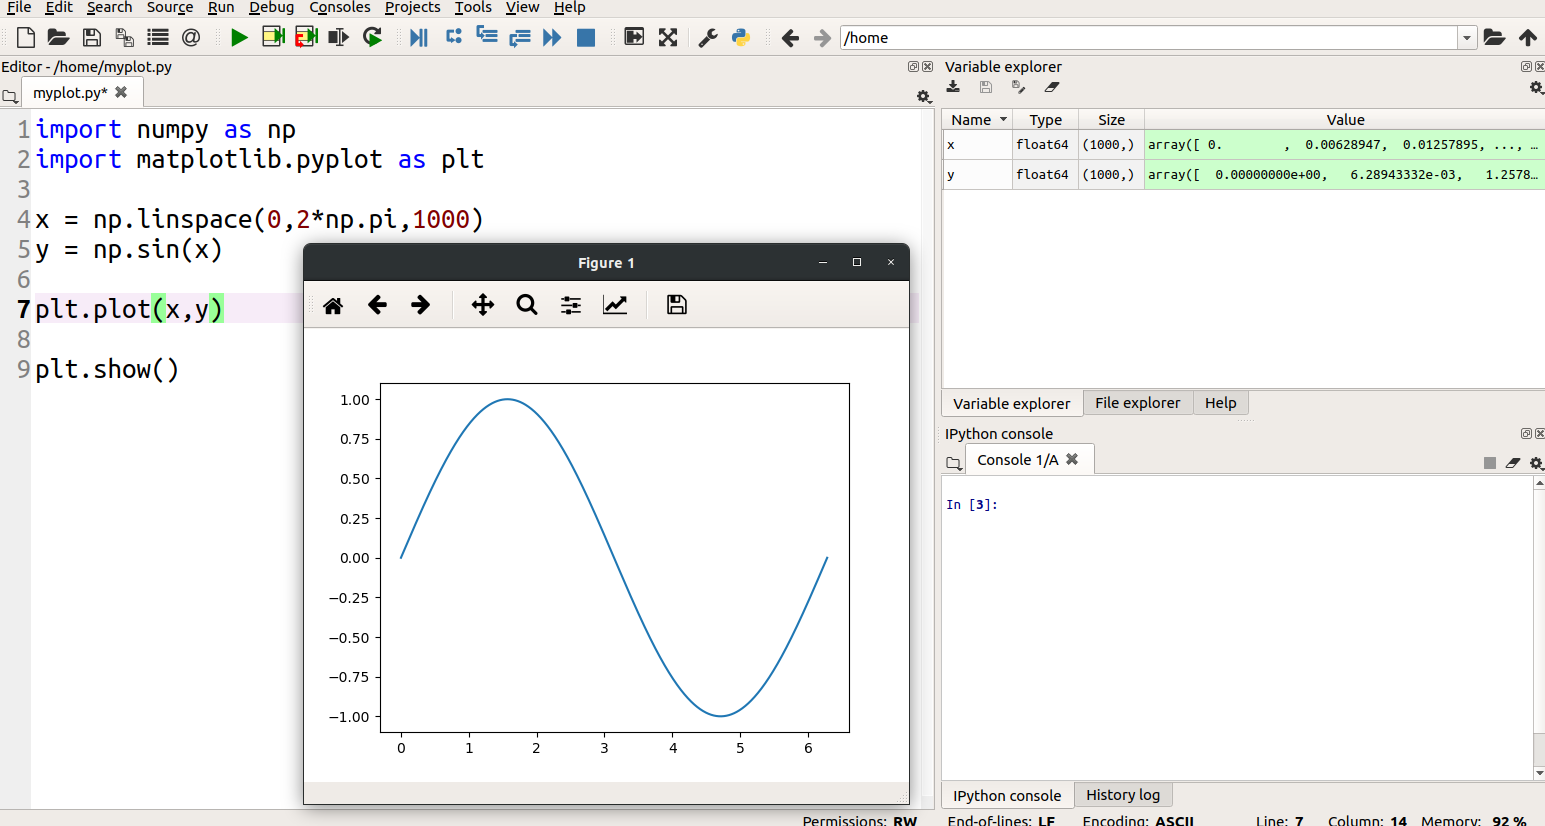
\includegraphics[width=\textwidth]{Figures/Spyder.png}
  \end{center}
\end{figure}

\subsection{Other Options}

It is possible to use
\href{https://colab.research.google.com/drive/1-VzSDojevQZ6A0oJNol9YXV6SRp3FKeP}{Google
  Colab} if you want to collaborate on Python projects or even get apps for your phone (\href{https://play.google.com/store/apps/details?id=ru.iiec.pydroid3&hl=en_US&gl=US}{Pydroid} or \href{https://apps.apple.com/us/app/pythonista-3/id1085978097}{Pythonista}
depending on Android or iPhone). You'll need to download 32 bit or 64
bit but which one? Well you need to figure out how many bits your
computer has. This is a great thing to Google. Type the following: "do
I have a 32 bit or 64 bit computer" into Google. I’m willing to bet
you have a 64 bit computer but you may as well check. We’ll learn
about the difference between 32 and 64 bit computers when we get to
the projects on Binary.

\subsection{Setting up your IDE}

Once you have Thonny or Spyder installed you need to install numpy and
matplotlib which are modules within Python that allow us to do some
extra things like numerical computation with Python (numpy) and Matlab
style Plotting libraries (matplotlib). I explain how to install
modules in my Youtube videos above; however, you need to head over to
Tools>Manage Packages in Thonny. You can see in the image below I
already have version 3.1.2 but I can upgrade to 3.2.2

\begin{figure}[H]
  \begin{center}
    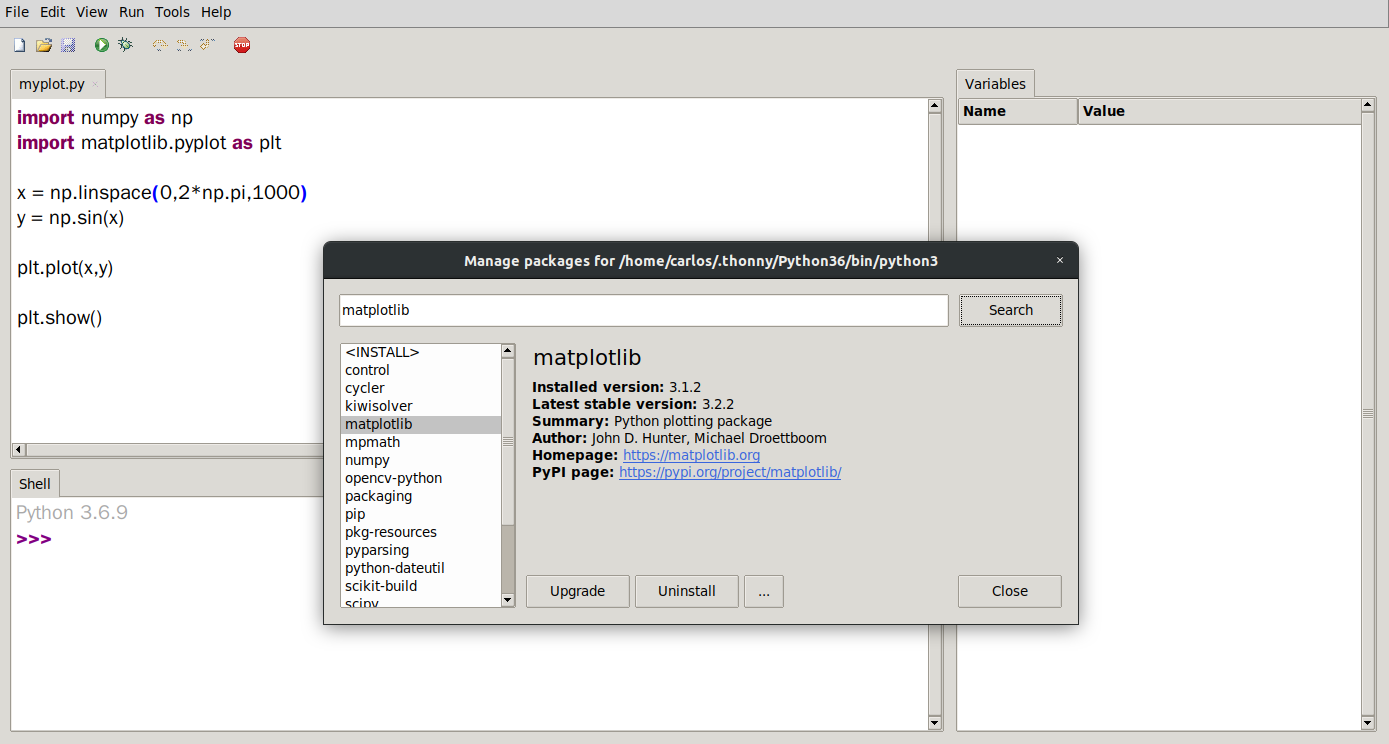
\includegraphics[width=\textwidth]{Figures/IDE_upgrades.png}
  \end{center}
\end{figure}

If numpy or matplotlib is not already included in Spyder then you need
to type the following into the Python Console in the lower right hand
corner of Spyder which is called the IPython console. 

\begin{verbatim}
!pip install matplotlib
\end{verbatim}

If that doesn’t work try

\begin{verbatim}
!pip3 install matplotlib
\end{verbatim}

You can see in the output example below that I already have matplotlib
installed as it says “requirement already satisfied”. Assuming you
have a valid internet connection it will install the necessary
module. 
\begin{figure}[H]
  \begin{center}
    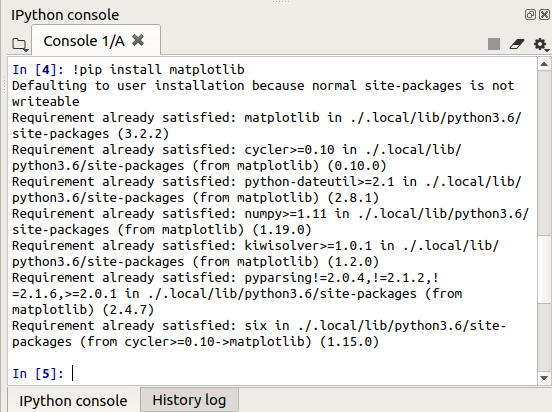
\includegraphics[width=0.5\textwidth]{Figures/console_thonny.png}
  \end{center}
\end{figure}

\subsection{Scripting}

Once you have numpy and matplotlib it’s time to make a plot. I have a
pretty \href{https://www.youtube.com/watch?v=7nAzHPURYW0&list=PL_D7_GvGz-v1RsDs_OdNW65qRjEjmpfQx&index=8}{comprehensive youtube video on how to plot in matplotlib} but if
you prefer text I will walk through a simple example.

\begin{figure}[H]
  \begin{center}
    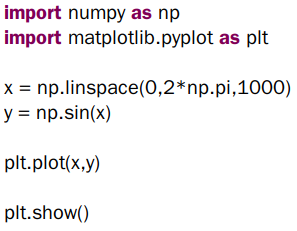
\includegraphics[width=0.5\textwidth]{Figures/matplotlib_example.png}
  \end{center}
\end{figure}

The code above will plot a sine wave from 0 to 2pi. The two lines at
the top are importing the numpy and matplotlib modules you installed
earlier. When they are imported we give them shorter names so it’s
easier to reference them so numpy will now be called np and
matplotlib.pyplot will be called plt. The next two lines then create a
vector “x” from 0 to 2pi using 1000 data points. The next line then
uses the sine function to create the vector “y”. Finally “x” and “y”
are plotted and the figure is instructed to pop up on your screen
using the show() function.


%% Now that you somewhat understand some of
%% this I’d like you to plot the following function: 

%% \begin{equation}
%%   T(t) = 60(1-e^{-5t})+30
%% \end{equation}

%% Plot the function from 0 to 10 seconds and label the x axis ‘Time
%% (sec)’ and the y-axis ‘Temperature (F)’. Add a grid as well. There are
%% some things that I have not explicitly shown you how to do. The reason
%% why is because I want to teach you how to fish for information.  

%% The first thing I recommend trying is to type in the commands in the
%% IPython console or the Shell. Type the first two commands below which
%% will show you every single function that numpy has available to you. 
%% \ \\

\subsection{Built-In Help Function and dir()}

Running code will always create syntax errors. Typing your syntax
error into Google will yield so many results you might get
lost. Sometimes it helps to know how to learn things just from your
computer. For example, type in the commands below in the IPython
console or the Shell.

\noindent {\it import numpy as np}\\
{\it dir(np)}
\ \\

\begin{figure}[H]
  \begin{center}
    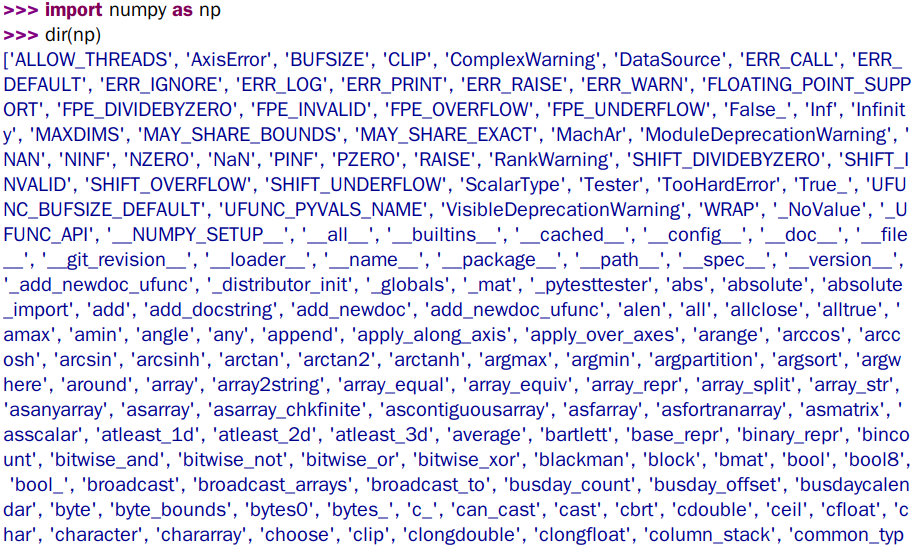
\includegraphics[width=\textwidth]{Figures/dir.png}
  \end{center}
\end{figure}

I included a photo of the output from the dir function. You’ll notice
there are a ton of functions in numpy. Every function in Python has a
\begin{verbatim} 
__doc__
\end{verbatim}

function. That’s two underscores followed by “doc” and then
another two underscores. If you’re ever curious about what a
particular function does you can just run the command below again in
the IPython console or Shell. In this example I’m looking at what
{\it arctan2} does.  

\begin{verbatim}
print(np.arctan2.__doc__)
\end{verbatim}

\begin{figure}[H]
  \begin{center}
    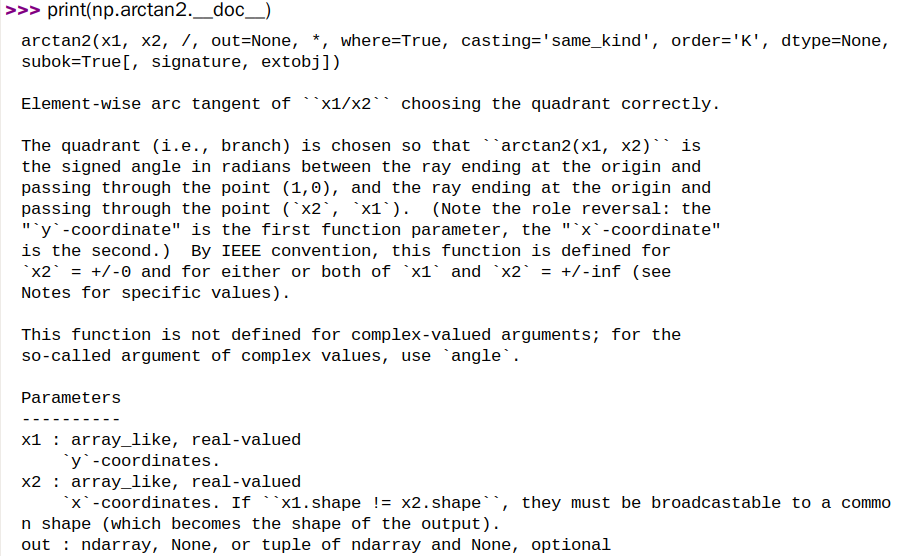
\includegraphics[width=\textwidth]{Figures/arctan2_doc.png}
  \end{center}
\end{figure}

You’ll see that arctan2 takes 2 input arguments “x1” and “x2”. I
didn’t include the entire output but if you continue to scroll through
the output it will even include examples on how to use the function.  

Another way to learn certain functions is by visiting the appropriate
documentation. The \href{https://numpy.org/doc/}{Numpy Docs} website
for example has all the documentation you need for Numpy. Navigating
that website you can find the same \href{https://numpy.org/doc/1.19/reference/generated/numpy.arctan2.html?highlight=arctan2#numpy.arctan2}{documentation for arctan2}.

As a last resort you can always Google “how to compute the inverse
tangent 2 function in Python”. Note though that there is so much
content out there on Google that you could easily get lost. Still,
there’s also so much information that the answers are out there for
just about anything.  

So you have three methods for finding out how to program in
python. The dir and {\it \_\_doc\_\_} functions in Python, using the appropriate
documentation online and of course Google. I’m lumping Youtube in with
Google which is also another way to learn information although when I
want to find information quickly I just use the documentation. It’s
the best in my opinion. 

\subsection{Assignment}

Your assignment for this project is to plot the equation below from 0 to 10 seconds and include that Figure in your report. You must add a grid and label the x-axis ‘Time (sec)’ and the y-axis ‘Temperature (F)’

\begin{equation}
  T(t) = 60(1-e^{-5t})+30
\end{equation}

Once you've completed the project above, upload a PDF with all of the photos and text
below included. My recommendation is for you to create a Word document
and insert all the photos and text into the document. Then export the
Word document to a PDF. For videos I suggest uploading the videos to
Google Drive, turn on link sharing and include a link in your
PDF. Note that all code must be included in the appendix or you'll be
penalized 10\%. 


\begin{enumerate}[itemsep=-5pt]
  \item Include a screenshot of your Python IDE (Thonny or Spyder is suggested) - 40\%
  \item Include the plot of temperature vs time being sure to save the figure so it is in high resolution - 40\%
\end{enumerate}


\section{Getting Started with the CPX/CPB}

\subsection{Parts List}
\begin{enumerate}[itemsep=-5pt]
  \item Laptop
  \item CPX(or CPB)
  \item USB Cable (with a data line. Not all USB cables have data
    lines)
\end{enumerate}

\subsection{Setting up your Circuit Playground}

By now you hopefully have your Circuit Playground (CPX) and it's time
to get your CPX up and running. A very in depth and detailed tutorial
can be found on the
\href{https://learn.adafruit.com/circuitpython-made-easy-on-circuit-playground-express/first-things-first}{Adafruit
  Learn site.} The text below is a summary 
of what you need to do to get the CPX up and running. 

When you get your CPX and plug it into the computer via USB it
actually won't run Python just yet. First you need to double click the
reset button (the button in the center. It says RESET above the
button) and put it into boot mode. All the neopixels (the ring lights
on the CPX) will light up green. 
\begin{figure}[H]
  \begin{center}
    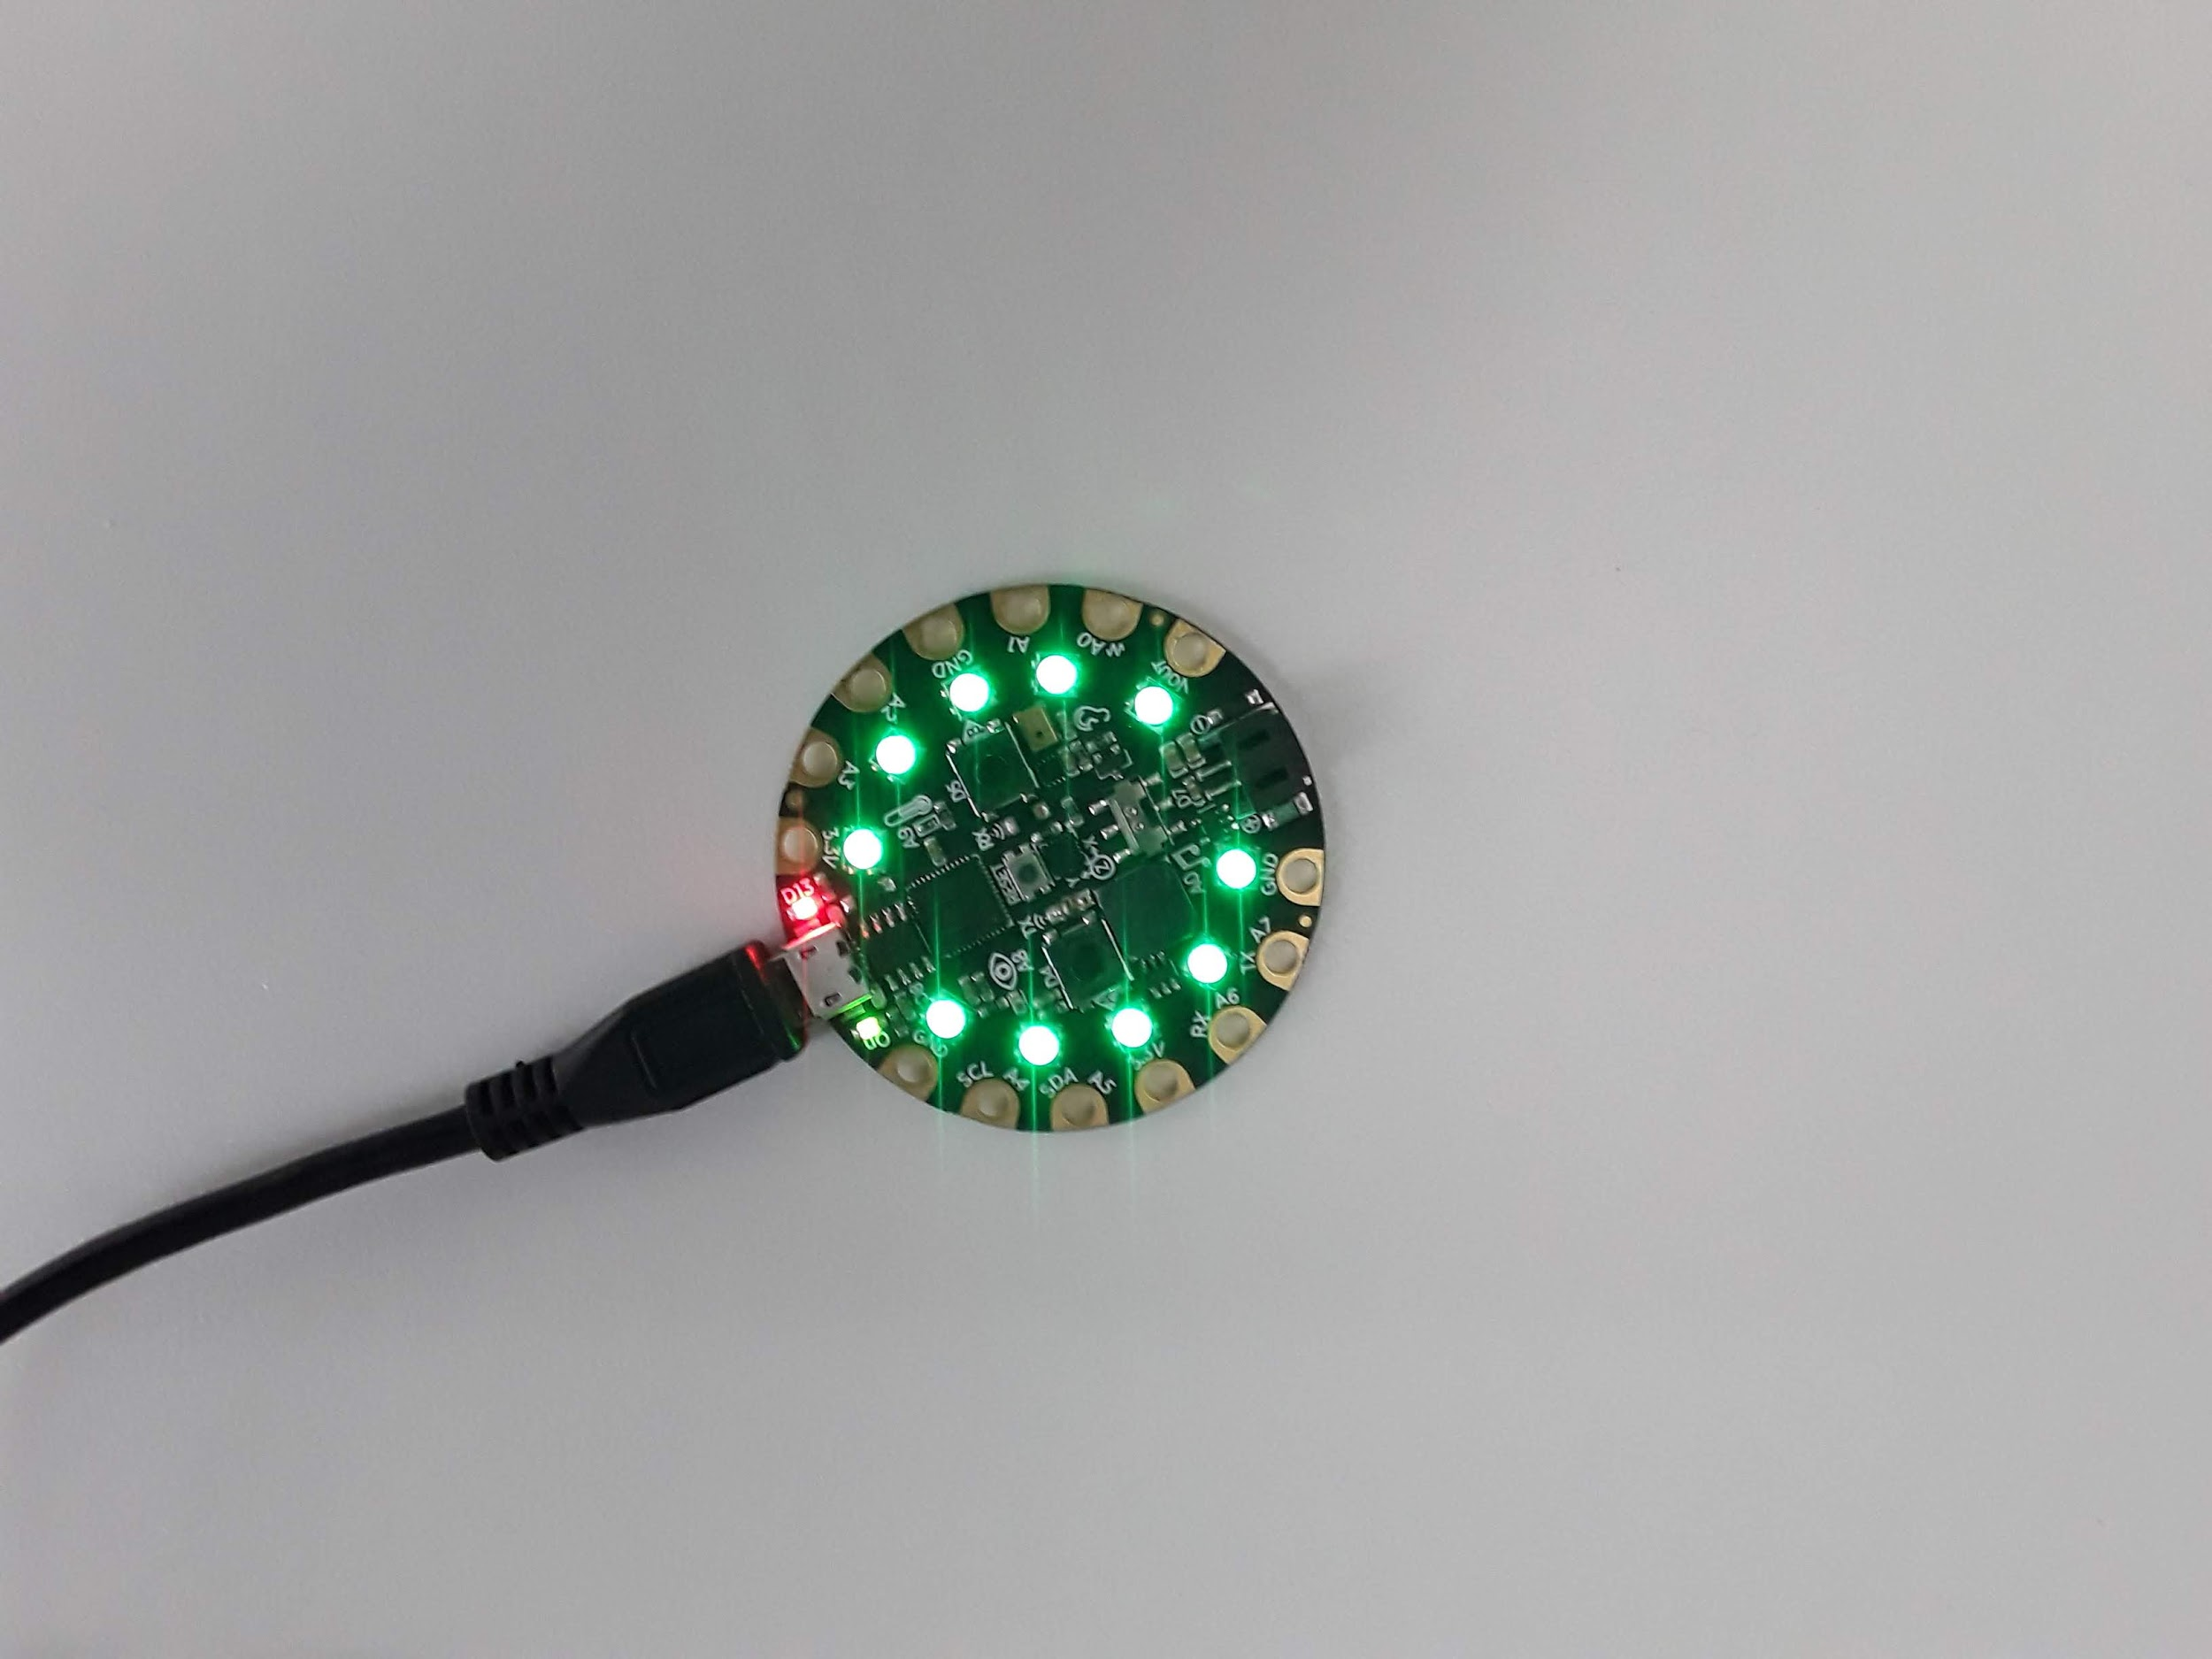
\includegraphics[width=\textwidth]{Figures/CPX_boot.jpeg}
  \end{center}
\end{figure}
Something called CPLAYBOOT will pop up on your computer just like a
USB stick or external harddrive. A couple files with be in there but
it doesn’t matter what they say right now.
\begin{figure}[H]
  \begin{center}
    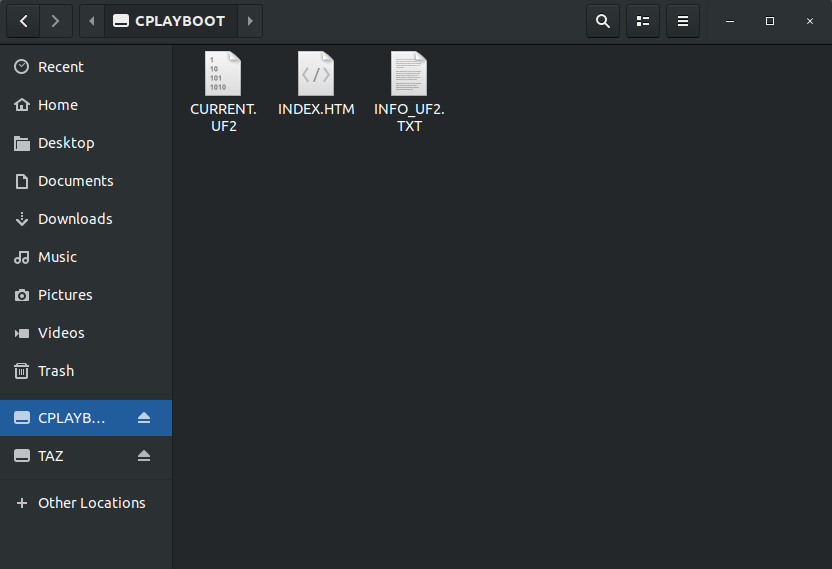
\includegraphics[width=\textwidth]{Figures/CPLAYBOOT.png}
  \end{center}
\end{figure}
You then need to download what’s called a \href{https://circuitpython.org/board/circuitplayground_express/}{UF2 file} and transfer it
onto the CPX. Note if you purchased a kit with the Bluefruit you need
to download a
\href{https://circuitpython.org/board/circuitplayground_bluefruit/}{different
  UF2}. Make sure you get the right one. Once the 
UF2 is downloaded you need to drag the UF2 over to the CPLAYBOOT drive
on your computer. After a bit of time a USB drive called CIRCUITPY
will pop up as a flash drive on your computer. The CPX is now like a
USB stick with 2MB of storage. 
\begin{figure}[H]
  \begin{center}
    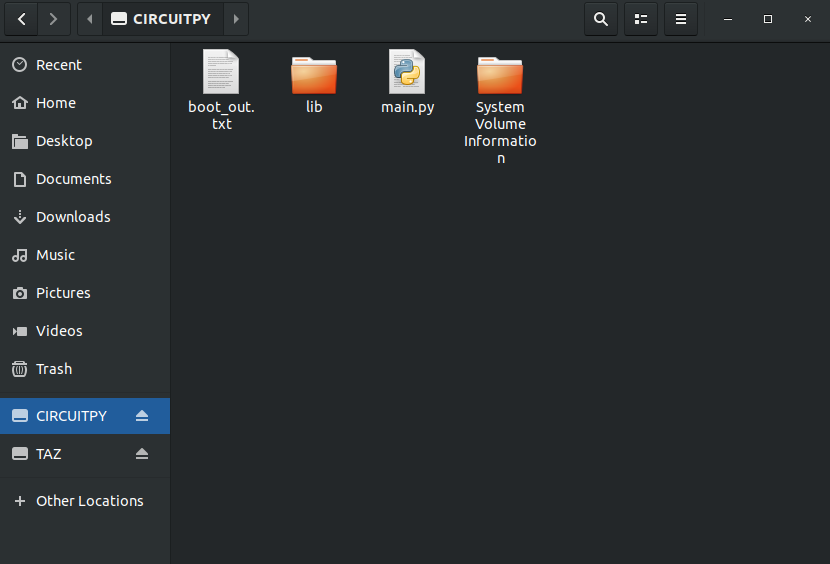
\includegraphics[width=\textwidth]{Figures/CIRCUITPY.png}
  \end{center}
\end{figure}
At this point the CPX is like a mini computer. If you put Python code
on the “flash drive” it will run python code. Since I’ve done this
before, there are a number of files already on my CPX. You may have
some or none of these. The “boot\_out.txt” file will tell you the
version of CircuitPython you have on the CPX. Mine says this:
\begin{verbatim}
Adafruit CircuitPython 5.3.0 on 2020-04-29; Adafruit CircuitPlayground Express with samd21g18
\end{verbatim}
Which means I have CircuitPython version 5.3.0 last updated on April
29th, 2020. The CPX itself is using the \href{https://www.microchip.com/wwwproducts/en/ATsamd21g18}{ATSAMD21G18}
microprocessor. The folder lib is a folder with extra libraries that
you may need to install later. The file main.py is the Python file
that the CPX is currently running. {\bf The CPX can store as many Python
files as possible for a 2MB flash drive but it will only run ONE
Python script at a time and that file must be named main.py} The folder
{\it System\_Volume\_Information} is a file management folder that we will
never use.

If you want the CPX to run code you simply need to edit the file
{\it main.py} or if that file does not exist you just need to create it. You
could just open Notepad or any other text app (Sublime,TexWrangler,
Emacs, Vi, Nano, Gedit, Notepad++, Wordpad, VSCode, etc) but the CPX
has alot of debugging options and it is recommended to use a program
called “\href{https://codewith.mu/en/download}{Mu}”. Mus is a good way to write and debug code on the
CPX. Note that Mu is only used to program the CPX. If you want to run
Python code on your laptop you need to use Thonny or Spyder (or
whatever other IDE you downloaded). If you want to run Python code on
your CPX you must use Mu. Once you’ve downloaded and installed Mu and
open it up it will look like this (Note it's possible the the software
gets updated from the time this book is published. As such be sure to
select the Circuitpython Mode for board development).
\begin{figure}[H]
  \begin{center}
    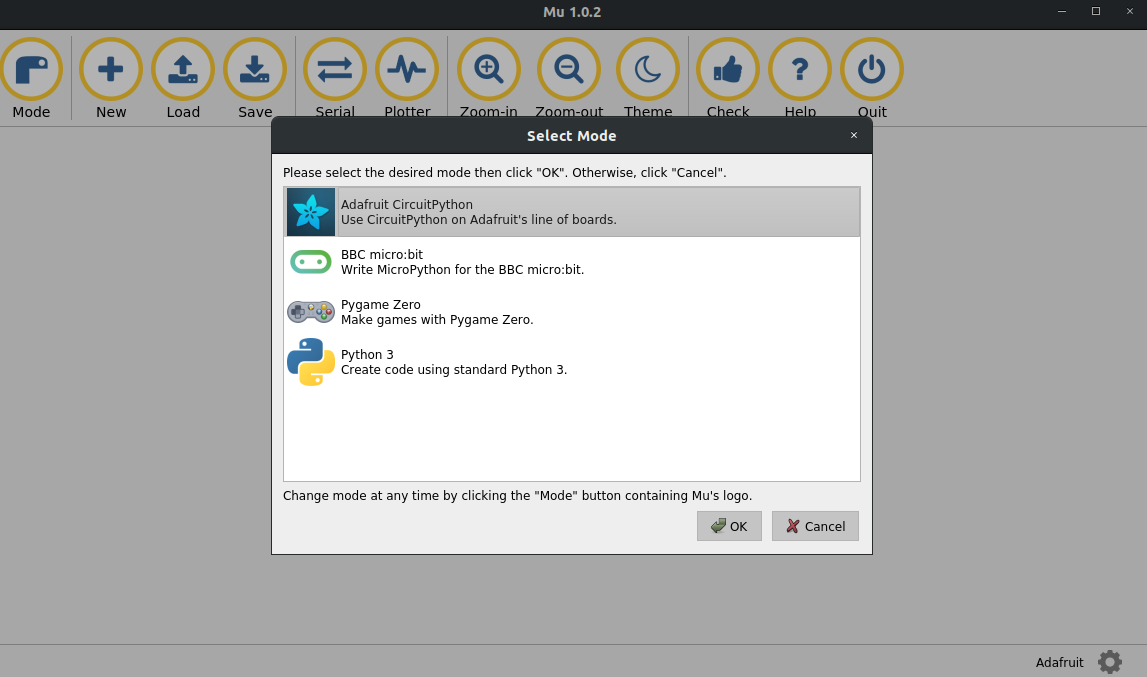
\includegraphics[width=\textwidth]{Figures/Mu.png}
  \end{center}
\end{figure}
Make sure to select the “Adafruit CircuitPython” option. If the
software has been updated and that option no longer exists, be sure to
select the option that says Circuitpython for board development.

Alright, let’s start writing code! If you have a file called {\it main.py}
on your CPX click the Load button and load {\it main.py} (make sure to load
the main.py that is stored on your CPX and not somewhere else on your
computer.) If a file {\it main.py} does not exist on your CPX simply click
the New button and then Save the file as {\it main.py} (again make sure you
save it to the CPX and not to your computer) 
\begin{figure}[H]
  \begin{center}
    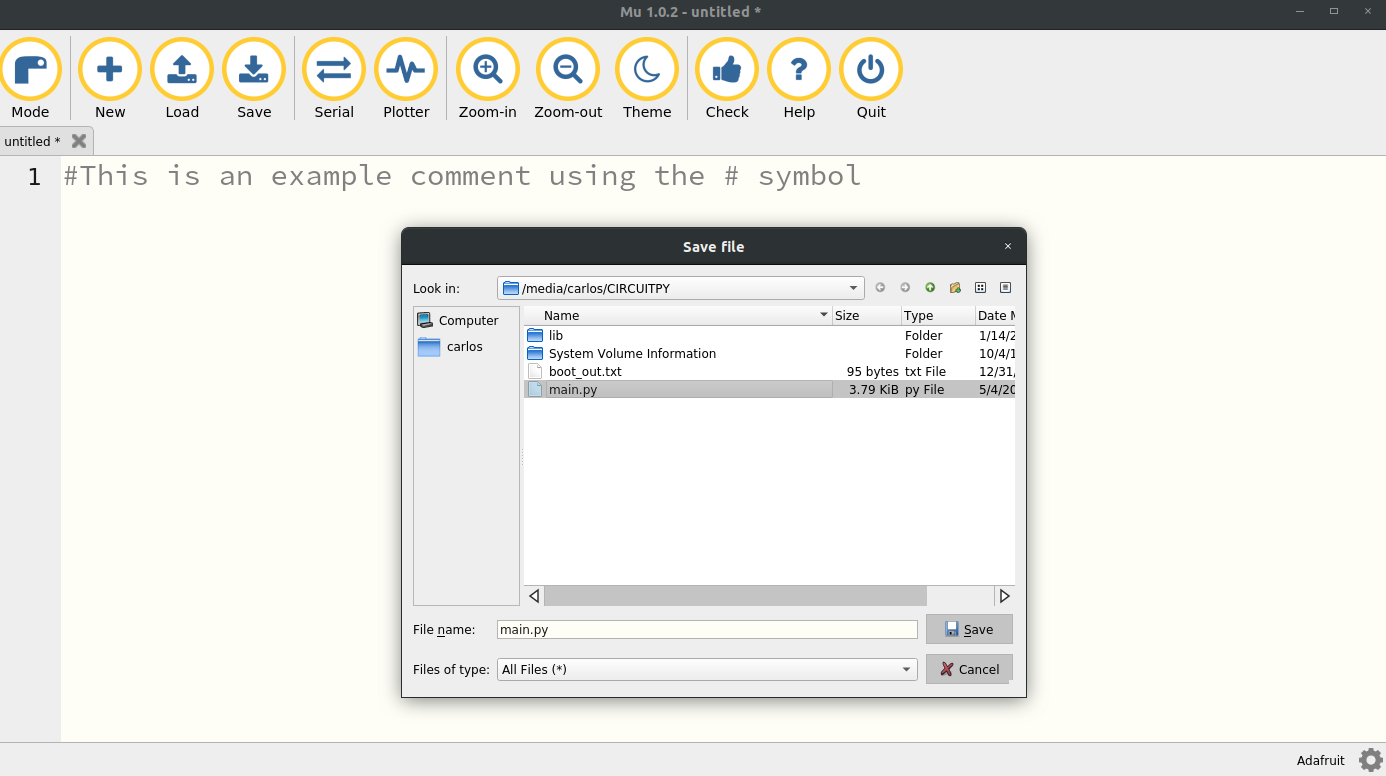
\includegraphics[width=\textwidth]{Figures/Mu2.png}
  \end{center}
\end{figure}
You’ll see that I am accessing the CIRCUITPY drive and saving the file
as main.py The file itself is empty and just has a comment using the \#
symbol. At this point since the file is blank the CPX won’t do
anything.

{\bf \it Now this is really important. Your CPX is a USB stick that can hold as
many Python files as 2MB will allow but it can only run or execute one
python script at a time. Furthermore it will only run two types of
files. It will run code.py if it exists and if it can't find code.py
it will run main.py If the CPX can't find main.py or code.y it will
just not do anything. If you have two versions of main.py or a
combination of main.py or code.py it will run one of them and not the
other. Make sure you only have one version of main.py or code.by but
not both! Some common things to check if your CPX isn't working. }
\begin{enumerate}[itemsep=-5pt]
  \item Make sure you're using Mu in the right Mode
  \item Make sure main.py or code.py is on the CIRCUITPY drive and not somewhere on your computer.
  \item Make sure you are editing the right file in Mu. Do you have two versions of main.py?
  \item Are you editing using Thonny or Spyder?
  \item Are you editing a file on your computer? Make sure you are writing to the CIRCUITPY drive.
  \item Unplug the CPX, close Mu and try again.
\end{enumerate}
So let’s get the CPX to do something simple like blink an LED. I have
an entire
\href{https://github.com/cmontalvo251/Microcontrollers}{Github}
devoted to Microelectronics. Specifically I have a
\href{https://github.com/cmontalvo251/Microcontrollers/tree/master/Circuit_Playground/CircuitPython}{folder
  with all of my Circuit Playground files}. The easiest program to 
run is the \href{https://github.com/cmontalvo251/Microcontrollers/blob/master/Circuit_Playground/CircuitPython/blink.py}{blink.py} script. I’ve attached a screenshot of the script
below. 
\begin{figure}[H]
  \begin{center}
    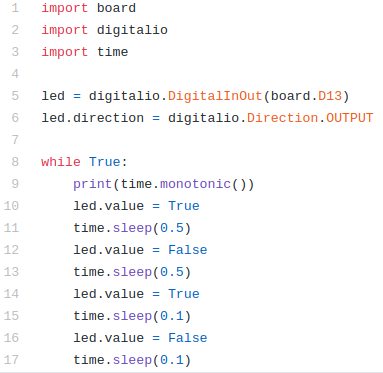
\includegraphics[width=\textwidth]{Figures/blink.png}
  \end{center}
\end{figure}
We will talk about what this code is doing later on. For now copy and
paste these 17 or so lines of code and paste them into Mu specifically
the {\it main.py} script. It will hopefully look like this.
\begin{figure}[H]
  \begin{center}
    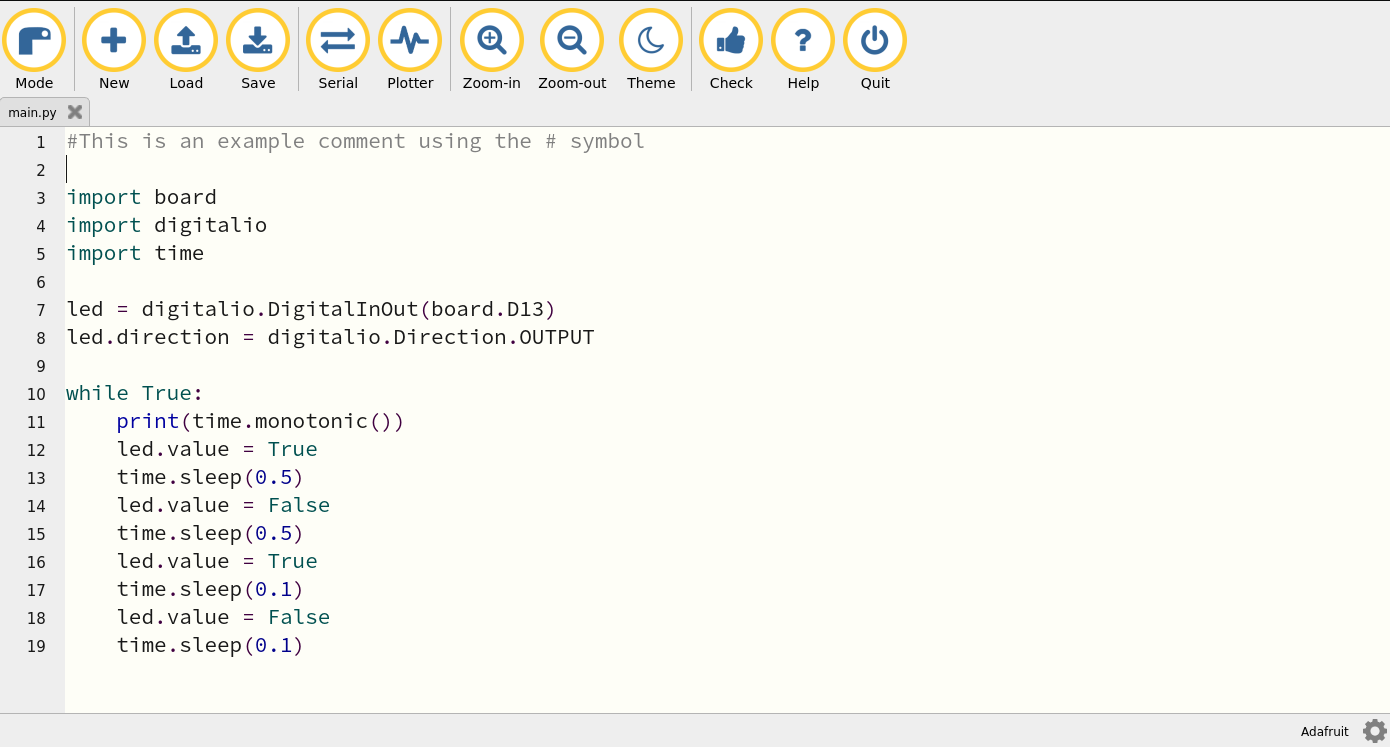
\includegraphics[width=\textwidth]{Figures/blinkmu.png}
  \end{center}
\end{figure}
Make sure to save. You can click {\it Zoom-In} and {\it Zoom-out} to zoom in and
out to change the font size and see more of the output. If the blink
code is working you will see a red led labeled D13 on the CPX blink
back and forth. D13 stands for digital pin 13. You’ll notice there are
analog pins labeled A5 and A6 among other numbers. Let’s talk about
the code a bit more and explain why it’s doing what it’s doing. The
three lines at the top of the code are {\it import} commands to import
different modules just like we did for {\it numpy} and {\it matplotlib}. In this
case the modules being imported are {\it board}, {\it digitalio} and
{\it time}. The module {\it board} is used to import the layout of the
CPX so we can access different pins on the CPX. The module {\it digitalio}
stands for digital input output which means we are inputting and
outputting digital signals. Since we can combine this module with the
{\it board} module we will be able to output digital signals to
different pins on the CPX board. Remember that PCB stands for printed
circuit board so {\it board} implies we are accessing pins on the CPX
PCB. Hopefully that makes sense. The final module we are importing is
{\it time} which acts just like the {\it time} module on your desktop
computer. It will let us access the CPX’s internal clock.

Moving along, lines 7 and 8 create an LED object using the {\it board}
module and {\it digitalio}. It’s a long line of code that basically says,
create a variable called {\it led} that lets us output a digital signal to
pin D13. We also set the direction of the LED to output since we only
want to write to the LED.

Lines 10 through 19 kick off an infinite loop that never ends. The
line that says {\it while True:} means loop while {\it True}. Well
{\it True} is always true which means it will loop forever. The colon
at the end of the line tells Python that the loop condition statement
ends and to begin looping from 11 through 19.

Line 11 specifically says {\it print(time.monotonic())}. First the
{\it print()} function is used to print things so that you and I can
see it. Rather than just seeing a blinking LED we want to see the time
printed. The {\it time.monotonic()} is using the module {\it time} which we
imported and using a function from that module called {\it monotonic()}
which calls the internal clock of the CPX. So how do you see the
output from the print statement? Hit the {\it Serial} button on Mu and you
will hopefully see some output. Here’s what it looks like on my
machine. 
\begin{figure}[H]
  \begin{center}
    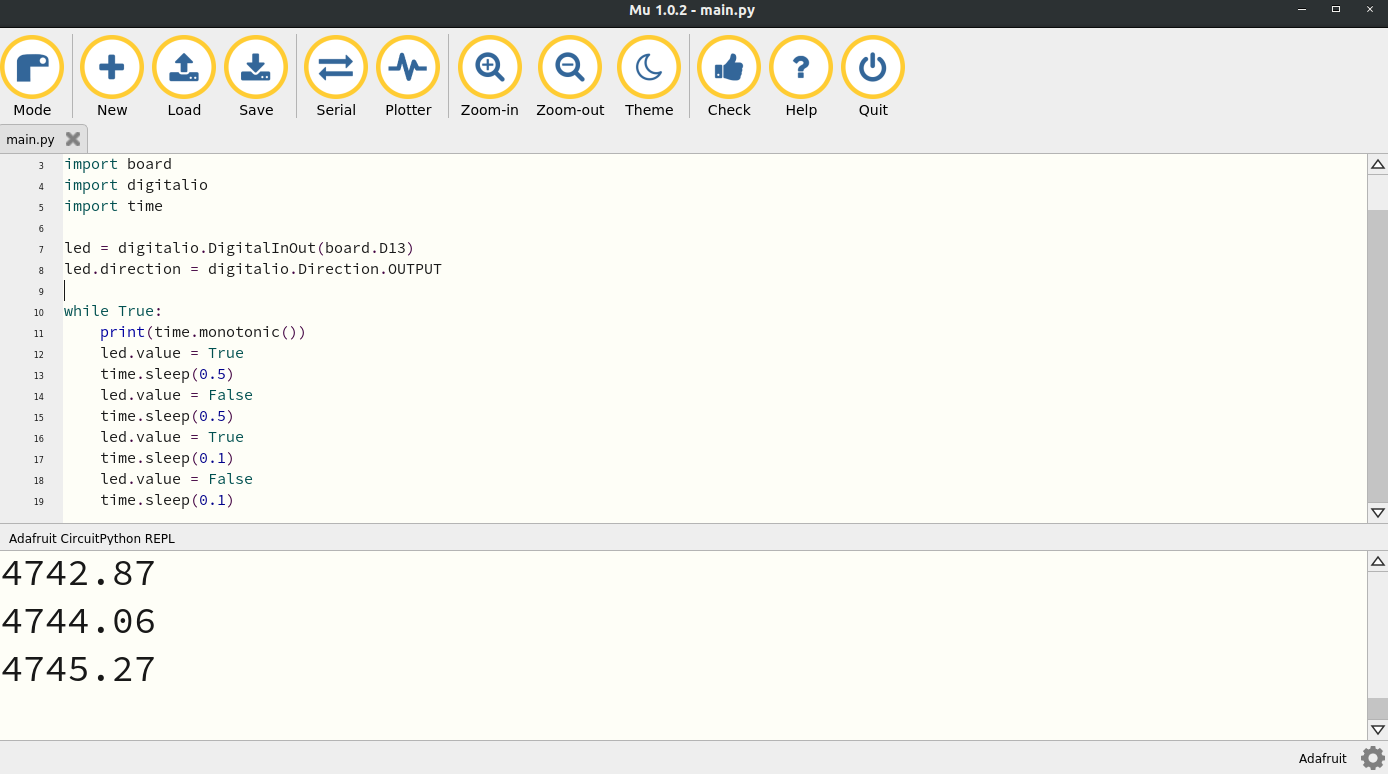
\includegraphics[width=\textwidth]{Figures/blinkmu2.png}
  \end{center}
\end{figure}
In this case you can see the time printed every time it goes through
the loop. You may even see an error. This {\it Serial} button is great for
debugging because it will tell you the error in your code. For
example, in the picture below I have an error in my code and the
{\it Serial} output is letting me know.
\begin{figure}[H]
  \begin{center}
    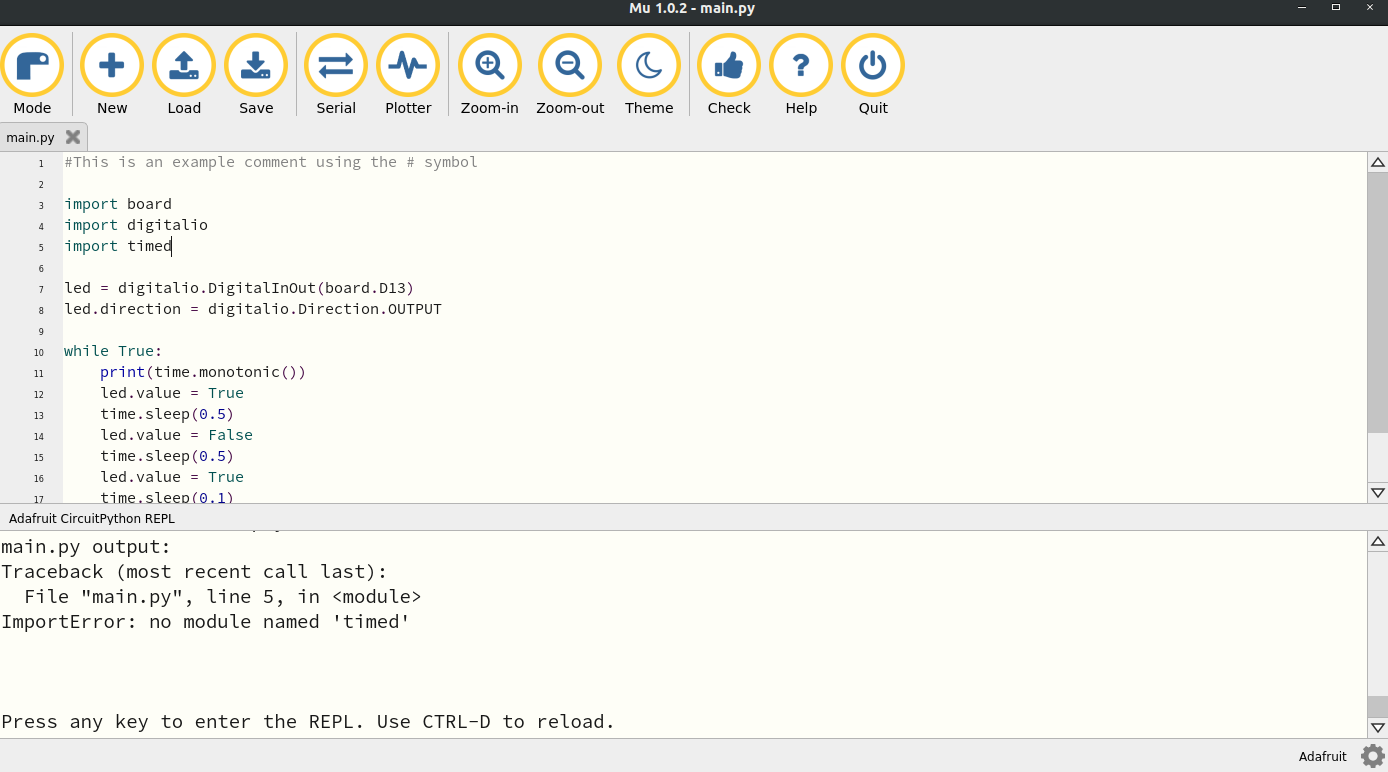
\includegraphics[width=\textwidth]{Figures/blinkerror.png}
  \end{center}
\end{figure}
In this case I have an error on line 5. It’s saying there is no module
named {\it timed}. The reason that module doesn’t exist is because the
module is actually {\it time} not {\it timed}. You can use the {\it
  Serial} monitor to check on your program and see what errors you may
have. Ok so there are two more lines of code to discuss. They are
{\it led.value = True} and {\it time.sleep(0.5)}.

These lines of code are repeated throughout the while loop and do two
things. First, the {\it led.value} either sets the value of the LED to
True which turns the light on or False which turns the light off. The
LED is digital which means the signal can either be on or off. There’s
no in between for digital signals. The {\it time.sleep()} function
tells the CPX to pause for half a second. You can change the number in
the parentheses if you want to change length of time the code
pauses. Note that the CPX completely pauses. That is no code runs
during a sleep.

If you’ve gotten the LED to blink you’re all set for this
lab. However, I’d like to you learn a few more things about
documentation. Just like Python on your desktop you can lookup the
documentation on the CPX itself. For example, I’ve added a print
statement to print the directory of time.
\begin{figure}[H]
  \begin{center}
    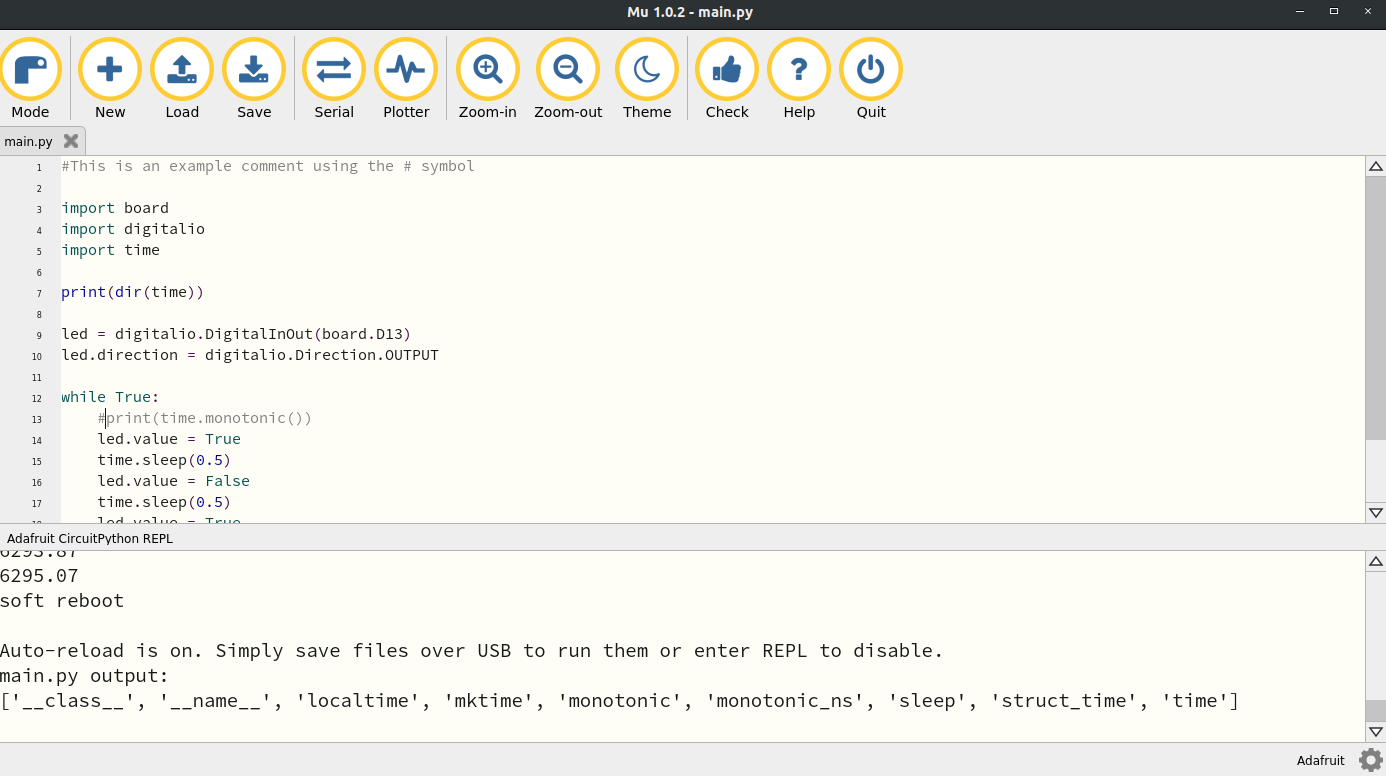
\includegraphics[width=\textwidth]{Figures/printtimeMu.png}
  \end{center}
\end{figure}
In this case I’ve added {\it print(dir(time))} to line 7. The output shows
that the {\it time} module has 9 functions including
{\it monotonic()}. Unfortunately CircuitPython does not have {\it \_\_doc\_\_}
functions built in which means if you want to learn about a specific
function, you need to visit the \href{https://circuitpython.readthedocs.io/en/5.3.x/README.html}{documentation for
CircuitPython}. Here’s the \href{https://circuitpython.readthedocs.io/en/latest/shared-bindings/time/index.html}{specific documentation for the} \href{https://circuitpython.readthedocs.io/en/latest/shared-bindings/time/index.html}{time}
\href{https://circuitpython.readthedocs.io/en/latest/shared-bindings/time/index.html}{module}. A lot of \href{https://github.com/adafruit/Adafruit_Learning_System_Guides/tree/master/CircuitPython_Essentials}{example code from the Adafruit Learning System is
also on Github.}

Finally, in order to keep practicing using Python on your desktop I
want you to modify the code above to run on your desktop
computer. You’re going to have to modify a few things. First, make
sure to open Thonny or Spyder depending on which version of Python IDE
you downloaded. Then, only import the {\it time} module. All the other
modules don’t exist on your desktop. Also, get rid of all the lines of
code that blink the LED. We just want to print time in a while
loop. Finally, the time module on your desktop uses a function called
time.time() (unless you have Python3 installed) so when you print time
make sure to use that module instead. Again visit the \href{https://docs.python.org/3/library/time.html#functions}{documentation
for time for Python if you want to learn more}. Thonny by default will
load Python version 3 but it’s possible you may have Python version 2
so make sure you look up the documentation for the appropriate version
of Python. After searching through the documentation you can use a
function called asctime() on your desktop. This is the output I get in
Thonny when I add a sleep of 1 second. The exercise for you is to do
something similar. 
\begin{figure}[H]
  \begin{center}
    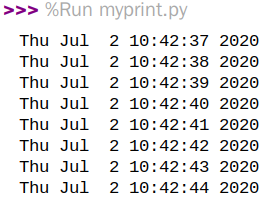
\includegraphics[width=\textwidth]{Figures/blinkcomputer.png}
  \end{center}
\end{figure}
\subsection{TL;DR}

\begin{enumerate}[itemsep=-5pt]
\item Plug in your CPX and double tap it to go into reset
  mode. CPLAYBOOT will mount to your computer. 
\item Download the \href{https://circuitpython.org/downloads}{UF2
  file}.
\item Drag the UF2 file to your CPLAYBOOT drive. After a few seconds
  CIRCUITPY will mount.
\item You need to then download
  \href{https://codewith.mu/en/download}{Mu}
\item Open Mu and make sure to select the mode Adafruit CircuitPython
\item Open main.py in Mu from the CIRCUITPY drive in Mu.
\item If code.py is on your CPX delete it
\item Copy the blink.py script into main.py
\item Once you have the script running, modify the script to run on
  your Desktop using Spyder or Thonny
\end{enumerate}

There is an accompanying
\href{https://www.youtube.com/watch?v=XFvLn6rwm3I}{youtube video to
  help you see me perform the 8 steps above.}

\subsection{Assignment}

Upload a PDF with all of the photos and text below included. My
recommendation is for you to create a Word document and insert all the
photos and text into the document. Then export the Word document to a
PDF. For videos I suggest uploading the videos to Google Drive, turn
on link sharing and include a link in your PDF.

\begin{enumerate}[itemsep=-5pt]
\item Include a screenshot of your computer showing the CIRCUITPY drive on your computer - 25\%
\item Copy and paste your blink.py code and write a paragraph explaining any changes you made to get it to work - 25\%
\item Take a video of you and your CPX blinking the LED. State your name, wave at the camera and show the CPX blinking (You must use software like OBS studio which records your screen and yourself. No cell phone videos allowed). - 25\%
\item Modify the blink.py code to run on your desktop computer in
  Spyder or Thonny. Copy and paste your desktop version of the code
  and screenshot the output. Include the code and the output in your
  submission - 25\%
\end{enumerate}


\section{Troubleshooting Guide}

{\bf Is your CPX/CPB broken or not running code? Read below.}

\begin{enumerate}[itemsep=-5pt]
  \item Your CPX is a USB stick that can hold as many Python files as 2MB will allow but it can only run or execute one python script at a time. It will look for code.py and then main.py and that's it. 
  \item Make sure you're using Mu in the right Mode (CircuitPython)
  \item Make sure main.py or code.py is on the CIRCUITPY drive and not somewhere on your computer.
  \item Make sure you are editing the right file in Mu. Do you have two versions of main.py or perhaps main.py and code.py?
  \item Do you have boot.py on there when you don't need it?
  \item Are you editing using Thonny or Spyder? You're supposed to use Mu. 
  \item Are you editing a file on your computer? Make sure you are
    writing to the CIRCUITPY drive.
  \item Do you have the right modules in your {\it lib} folder?
  \item Unplug the CPX, close Mu and try again.
  \item First, try and reset the CPX to CPLAYBOOT and reflash the UF2 to see if that fixes it.
  \item If you have a linux computer you can ``sudo screen /dev/ttyACM0" and then run ``import storage" and then ``storage.erase\_filesystem()"
  \item If that doesn’t work sometimes you just need to completely erase the CIRCUITPY drive so head over to this \href{https://learn.adafruit.com/adafruit-circuit-playground-express/troubleshooting}{troubleshooting guide} and follow some of the steps they tell you.
  \item As a last resort you can try to download these UF2s and
    hopefully it will fix all errors and mistakes -
    \href{https://cdn-learn.adafruit.com/assets/assets/000/048/745/original/flash_erase_express.ino.circuitplay.uf2?1512152080}{CPX}, \href{https://cdn-learn.adafruit.com/assets/assets/000/082/950/original/CP_Bluefruit_QSPI_Erase.UF2?1572026649}{CPB}
  \item If you're having an issue with an old bootloader be sure to update the \href{https://learn.adafruit.com/adafruit-circuit-playground-bluefruit/update-bootloader-use-command-line}{bootloader}. At the time of this writing here is the command you need to upload the new bootloader {\it adafruit-nrfutil --verbose dfu serial --package feather\_nrf52840\_express\_bootloader-0.8.0\_s140\_6.1.1.zip -p /dev/ttyACM0 -b 115200 --singlebank --touch 1200}. Note that the -- is a double dash and - is just one dash. Also this is for the feather\_nrf52840. You need to download the zip specific for the CPB by clicking the bootloader link. 
  \item Are you running out of memory? To figure out how much RAM you have on your CPX/CPB you need to {\it import gc} then run {\it gc.collect()} and then {\it print(gc.mem\_free())}. At the time of this writing, the CPX has about 17 KB of RAM and the CPB has around 140 KB of RAM. 
\end{enumerate}


\section{External LEDs and Push Buttons}

\subsection{Parts List}


\begin{enumerate}[itemsep=-5pt]
  \item Laptop
  \item CPX + USB Cable
  \item 2 Alligator clips
  \item Push Button
  \item Breadboard
  \item LED (Light Emitting Diode) (x3 in case you fry some)
  \item Resistor (300 to 1000 Ohms)
\end{enumerate}

\subsection{Learning Objectives}

\begin{enumerate}[itemsep=-5pt]
\item The VOUT and 3.3V pin are always "ON" even when code is not
  running on the CPX. So long as your CPX is plugged in via USB or a
  Lipo Battery
\item LED are Light Emitting {\bf Diodes} which means current only flows in one direction
\item LEDs need resistors in series otherwise they will get too hot and burn up
\item Breadboard pinout diagrams
\item Analog pins can be controlled by simply using the digitalio module
\item LEDs can be hooked up to analog pins and set to blink by changing the board pin
\end{enumerate}

In this project we’re going to use the same blink code as before but
modify it to blink an external LED. The purpose of this lab is to
familiarize yourself with the pins on the CPX and create a simple
circuit using the 5V pin on the CPX and one of the Analog pins. Your
laptop has a battery with something between 10 to 20V. There are DC to
DC converters in your laptop that provide 5V to your USB ports. These
USB ports can be used to power your CPX as you have done in the past
few labs.

If you purchased the optional
\href{https://www.adafruit.com/product/3287}{battery pack} you can
also power the CPX using 3 AA batteries. These batteries nominally
have 1.5 V but fully 
charged it's actually something like 1.8 V. So 1.8 times 3 is 5.4V
which is enough to power the CPX. If you have the battery pack and
some AA batteries, give it a try. If you still have the blink code
from the last project on board you’ll see the D13 LED blink as
before. You won’t be able to see the serial print() output as before
but that code will be running which is why D13 is blinking. {\bf I have
noticed that some of the battery packs have power and ground wires
swapped. If the battery pack doesn’t work it may be because those two
wires are backwards.}

The CPX itself uses 3.3V logic which means when it converts numbers to
binary a 0 (False) represents 0 volts and a 1 (True) represents
3.3V. The CPX has ports that are labeled various things. GND stands
for ground and you need to hook the negative end of your circuit to
this and it also has VOUT which supplies 5V to any circuit you
build. Hook the positive end of your circuit to the VOUT pin. There is
also a port labeled 3.3V and obviously that outputs 3.3V

You’re going to need to use a breadboard so if you’re not familiar
with how breadboards work I would recommend watching this \href{https://www.youtube.com/watch?v=mE33WpRWrXs}{video on how
breadboards work}. Your lab today specifically involves an external
LED. You can read about
\href{https://learn.sparkfun.com/tutorials/light-emitting-diodes-leds/}{LEDs}
more online if you wish. {\bf Remember that the long leg of the LED is 
the positive end and the short leg is the negative end.} The task today
is to wire an LED up to the CPX in the following ways

{\bf Whenever you modify a circuit on the breadboard, always be sure
  to remove power from the CPX. You can damage multiple components if
  you’re not careful.}

\subsection{LED with no Code}

For this part we are going to light up the LED without the use of any
code on the CPX. First, wire up the circuit with the positive end
connected to 5V. This is how my circuit looks. Make sure to use a
resistor between 300 and 1000 Ohms. An LED does not have that much
internal resistance so you need a resistor in series with an LED to
reduce the amount of current flowing through the LED or the entire LED
will fry. If you use a resistor that has too much impedance the LED
just won’t turn on because the voltage/current through the LED will be
below the activation voltage of the circuit. 
\begin{figure}[H]
  \begin{center}
    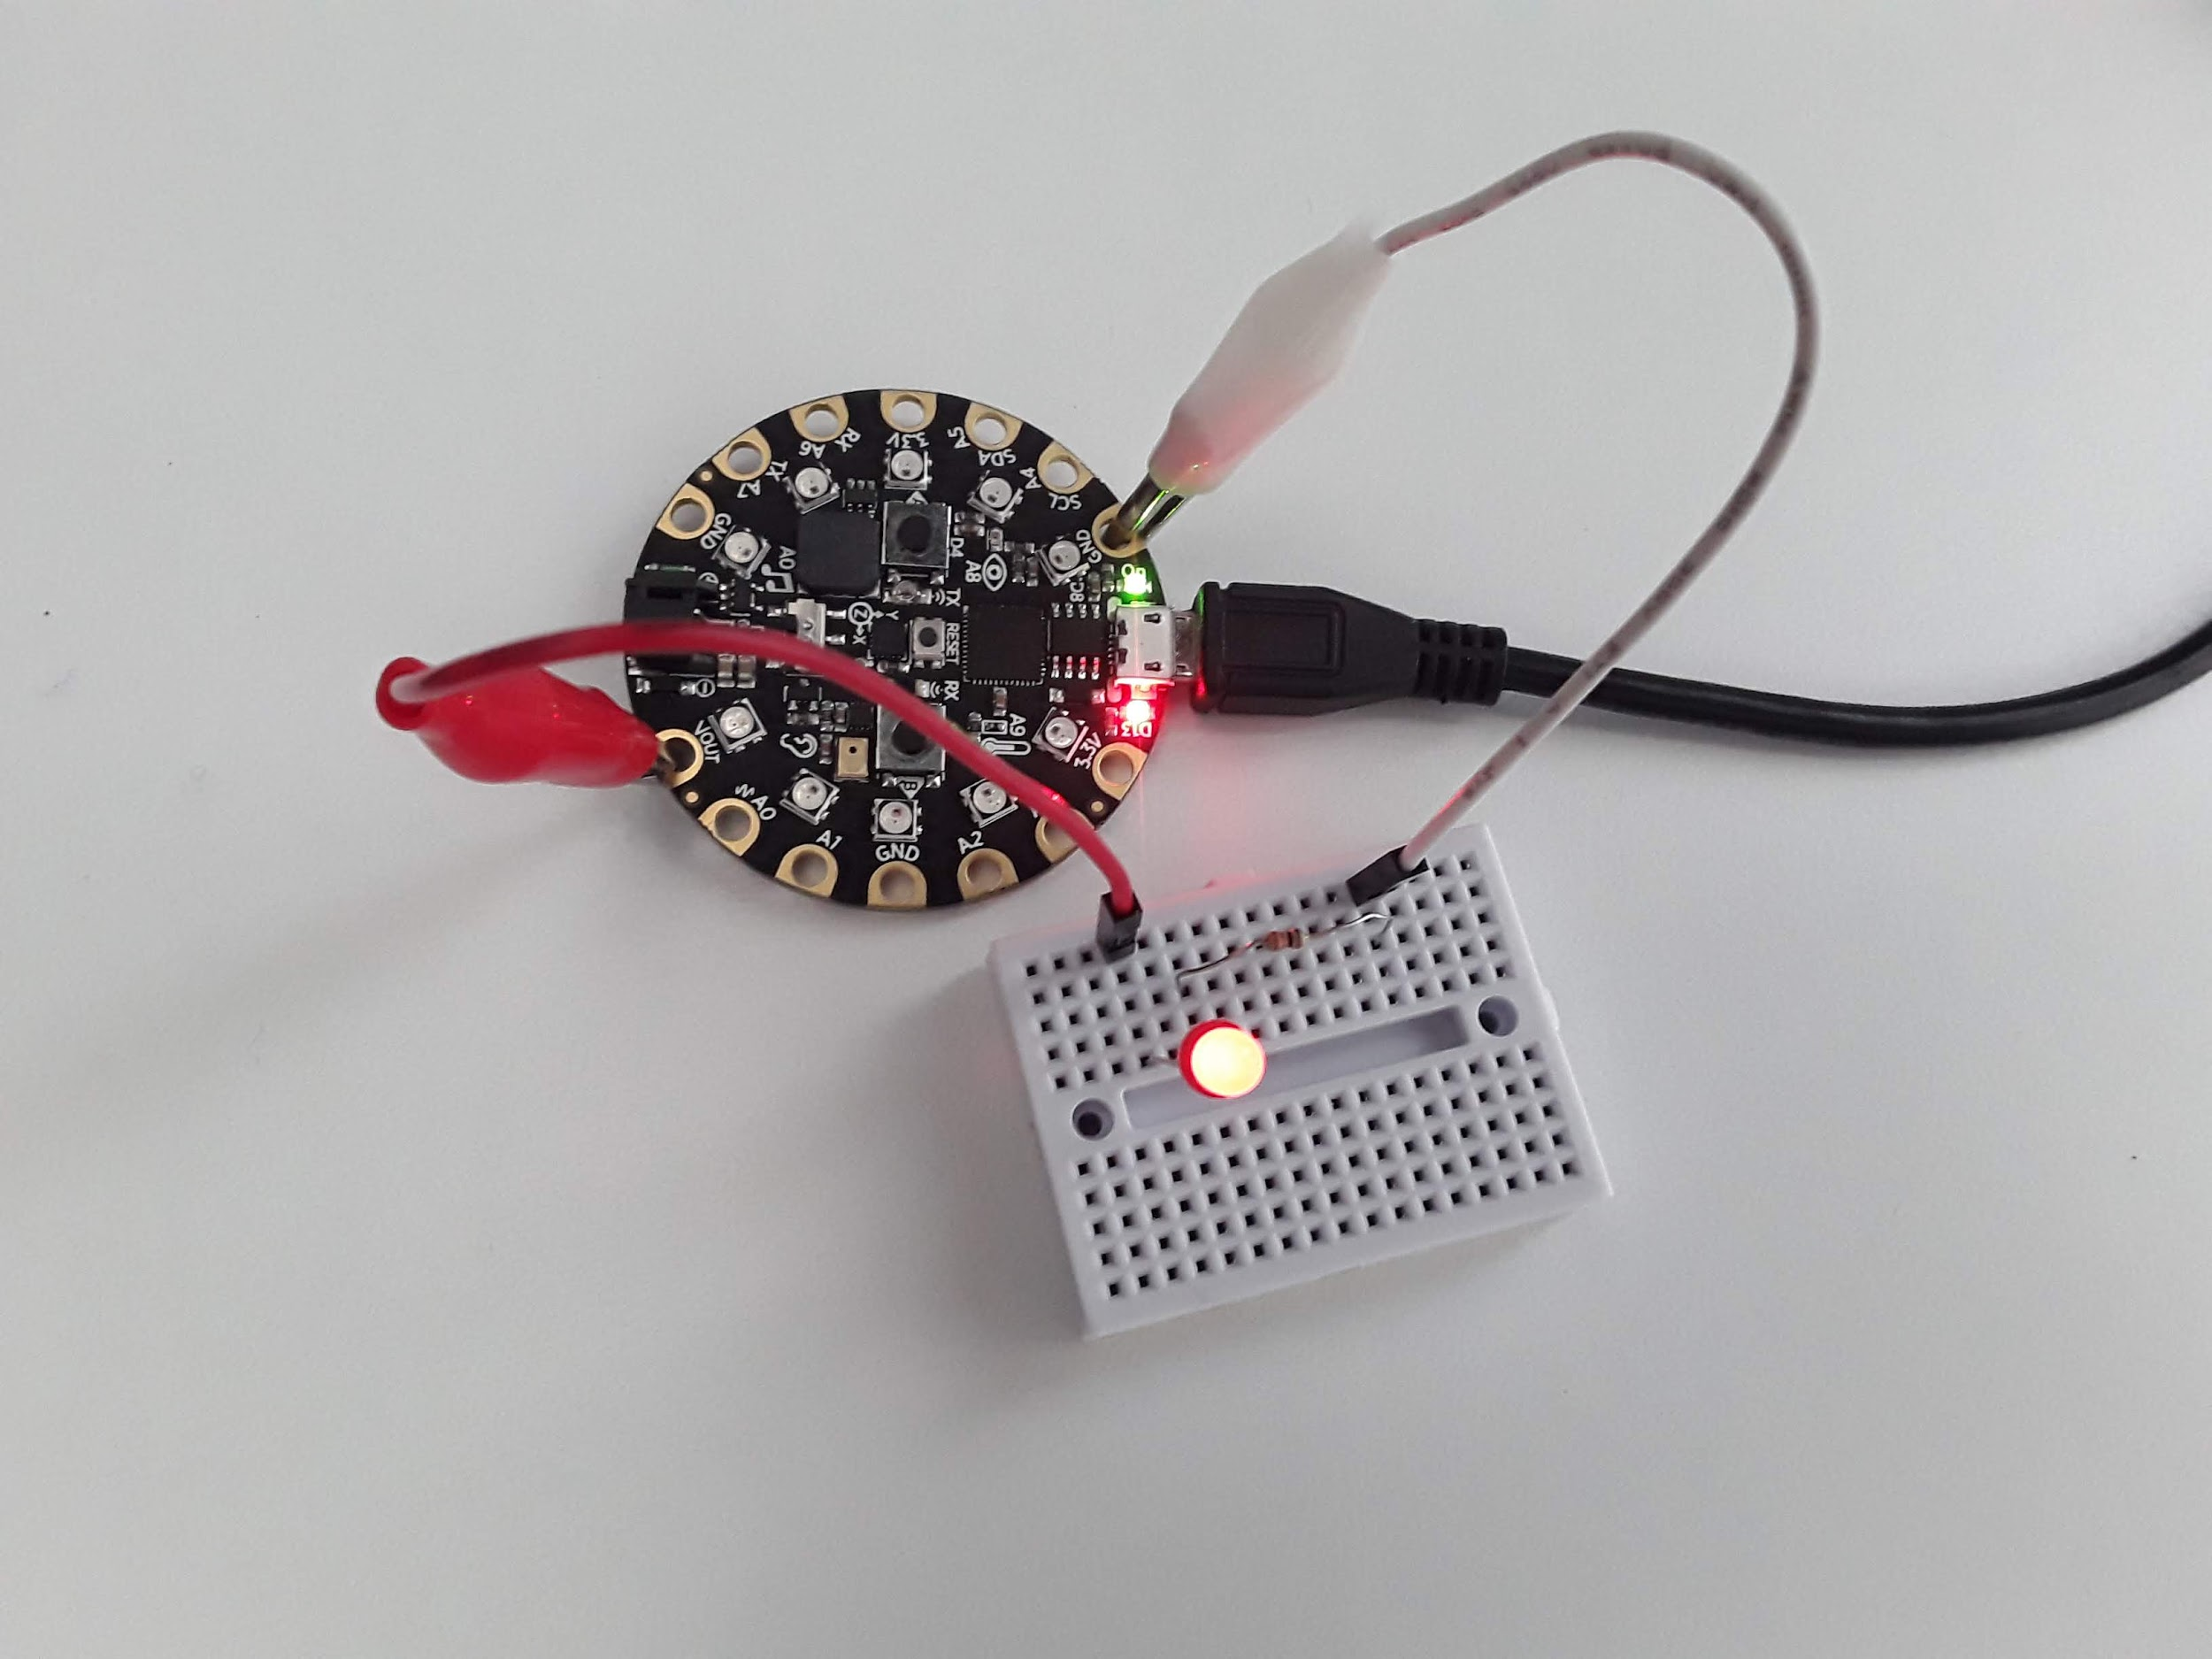
\includegraphics[width=\textwidth]{Figures/LED1.jpeg}
  \end{center}
\end{figure}
Once you have that circuit working, wire up the circuit again with the
3.3V output. Do you notice anything different when you hook up the
circuit with different pins? Here’s my circuit. Do you notice
something different about the intensity of the LED? Why is it
different?
\begin{figure}[H]
  \begin{center}
    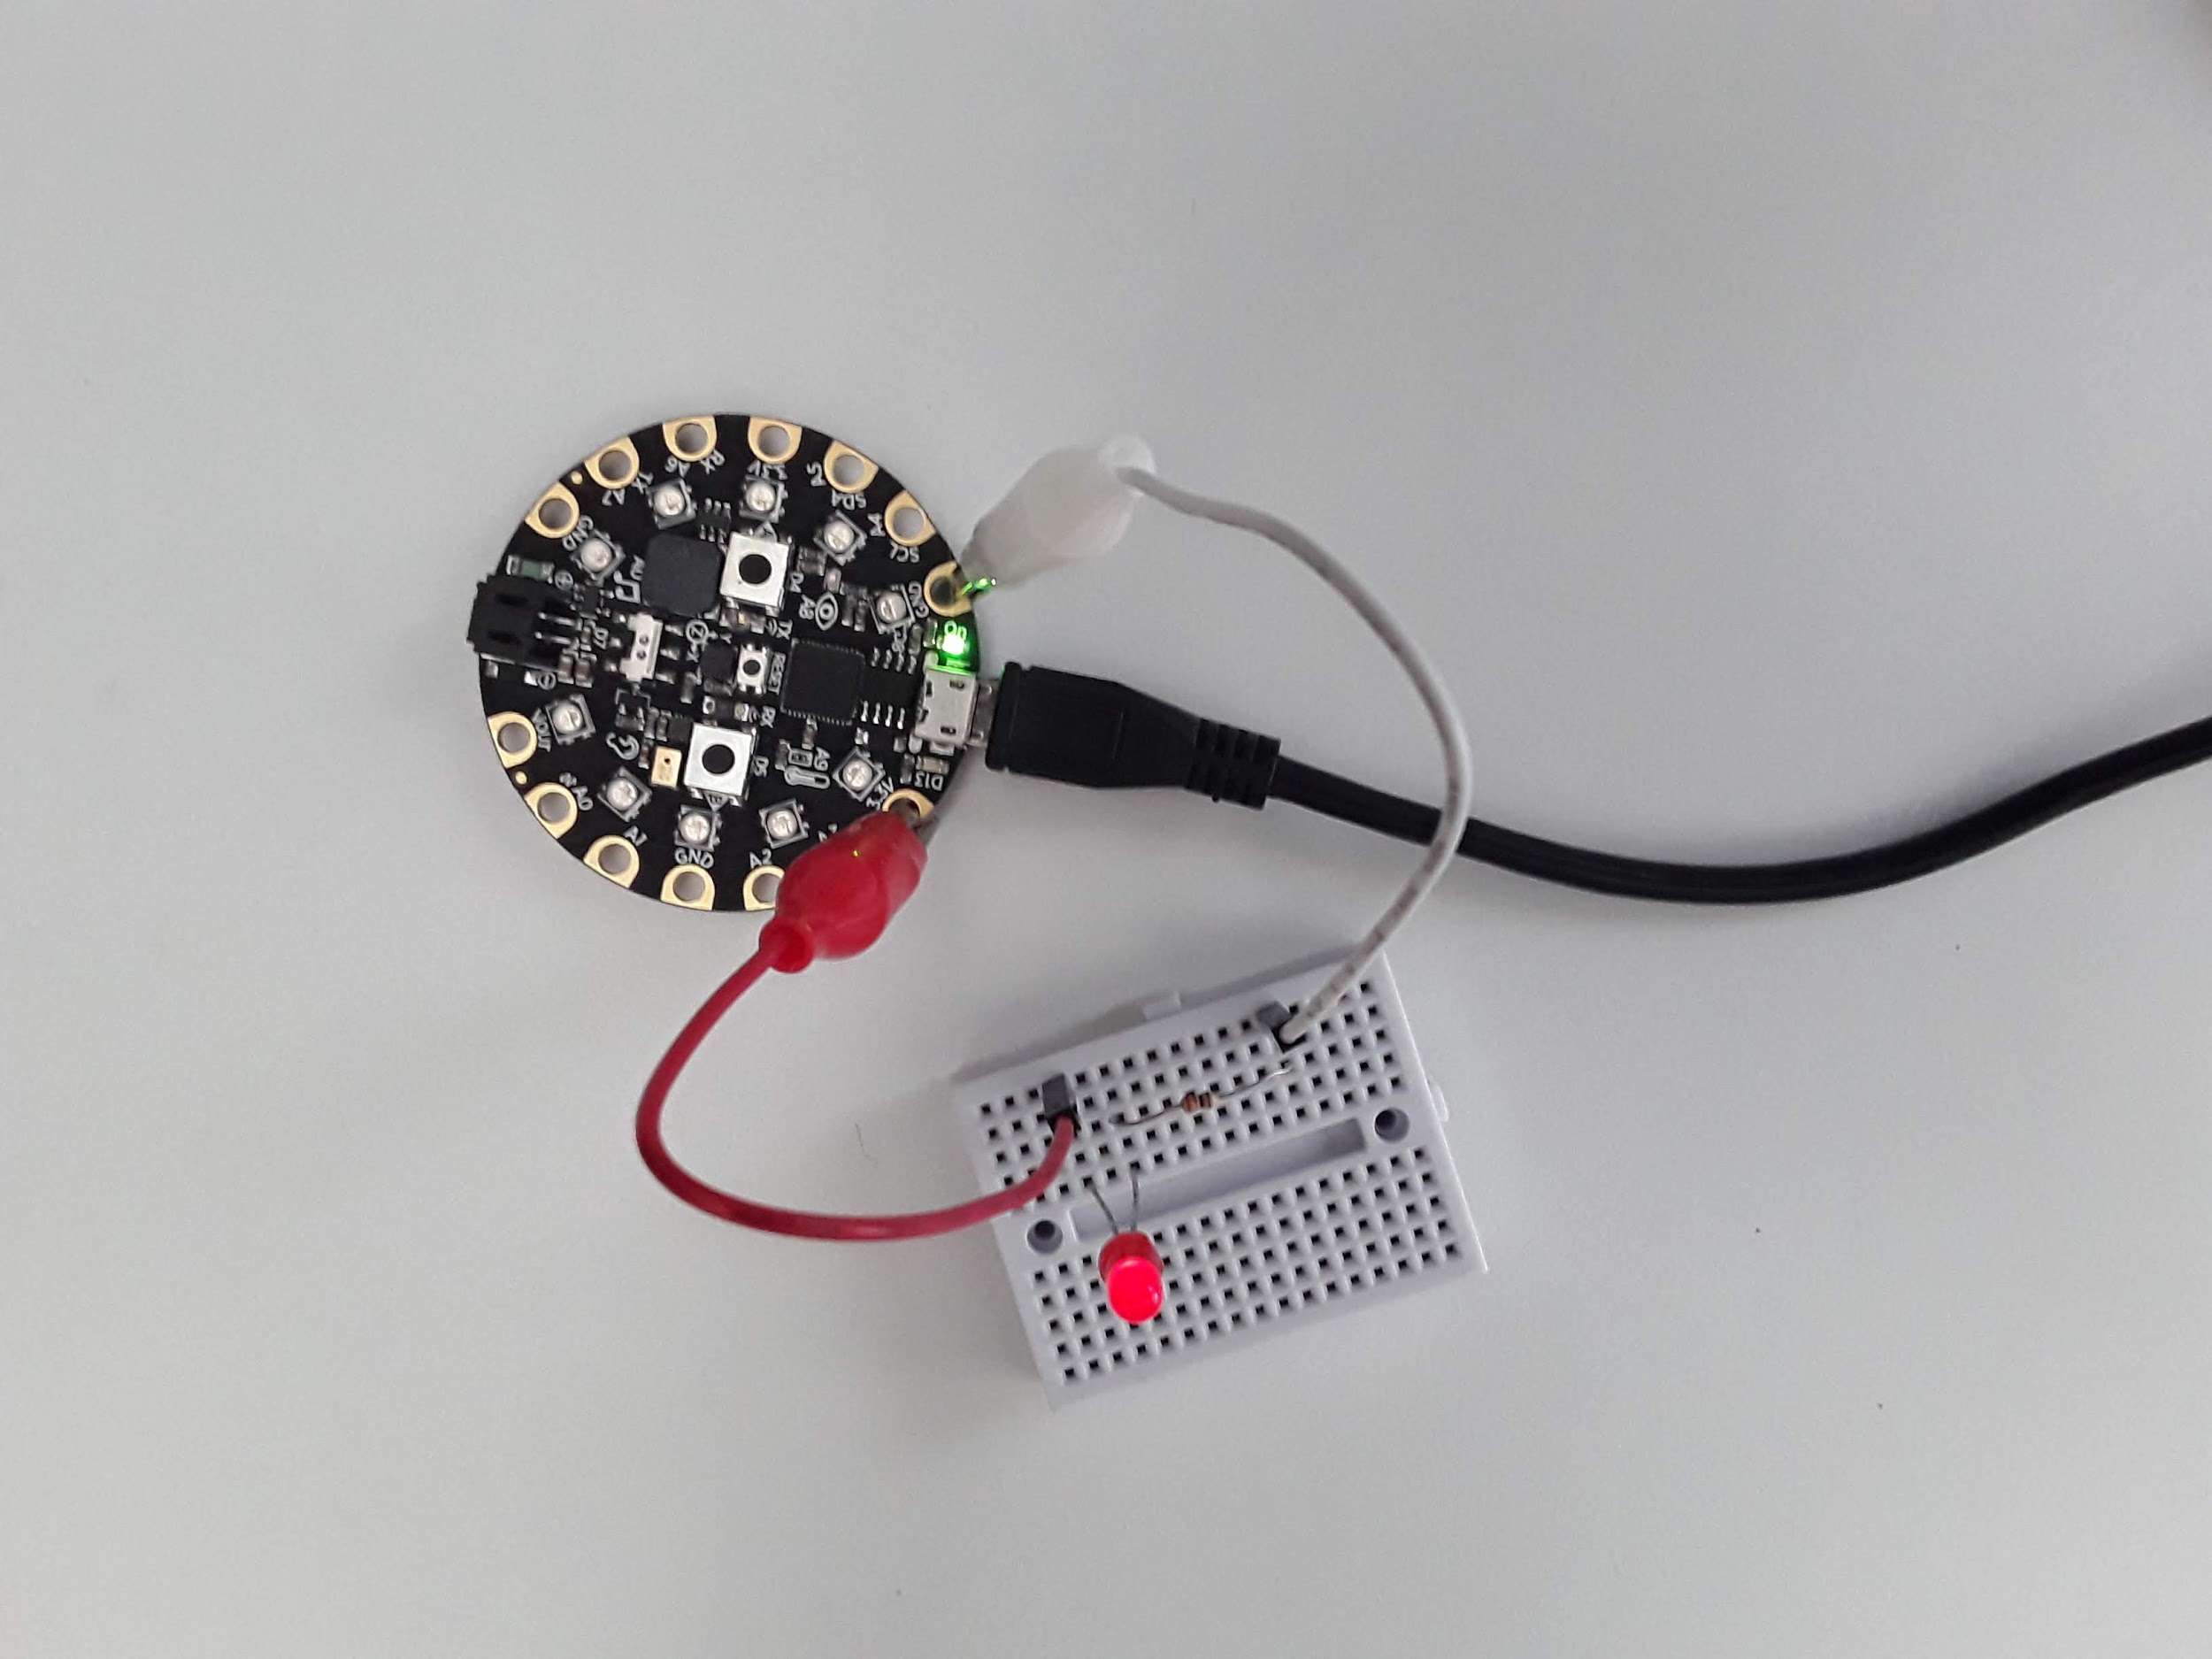
\includegraphics[width=\textwidth]{Figures/LED2.jpeg}
  \end{center}
\end{figure}
\subsection{LED with a push button}

Now that we understand breadboards a bit, we’re now going to manually
blink the LED using a push button placed 
onto the breadboard and have it act like a switch. Therefore, when the
button is pressed, the LED will turn on and when the button is
released the LED will turn off. The button just acts like a wire so
you can plug in the button anywhere in the circuit.
\begin{figure}[H]
  \begin{center}
    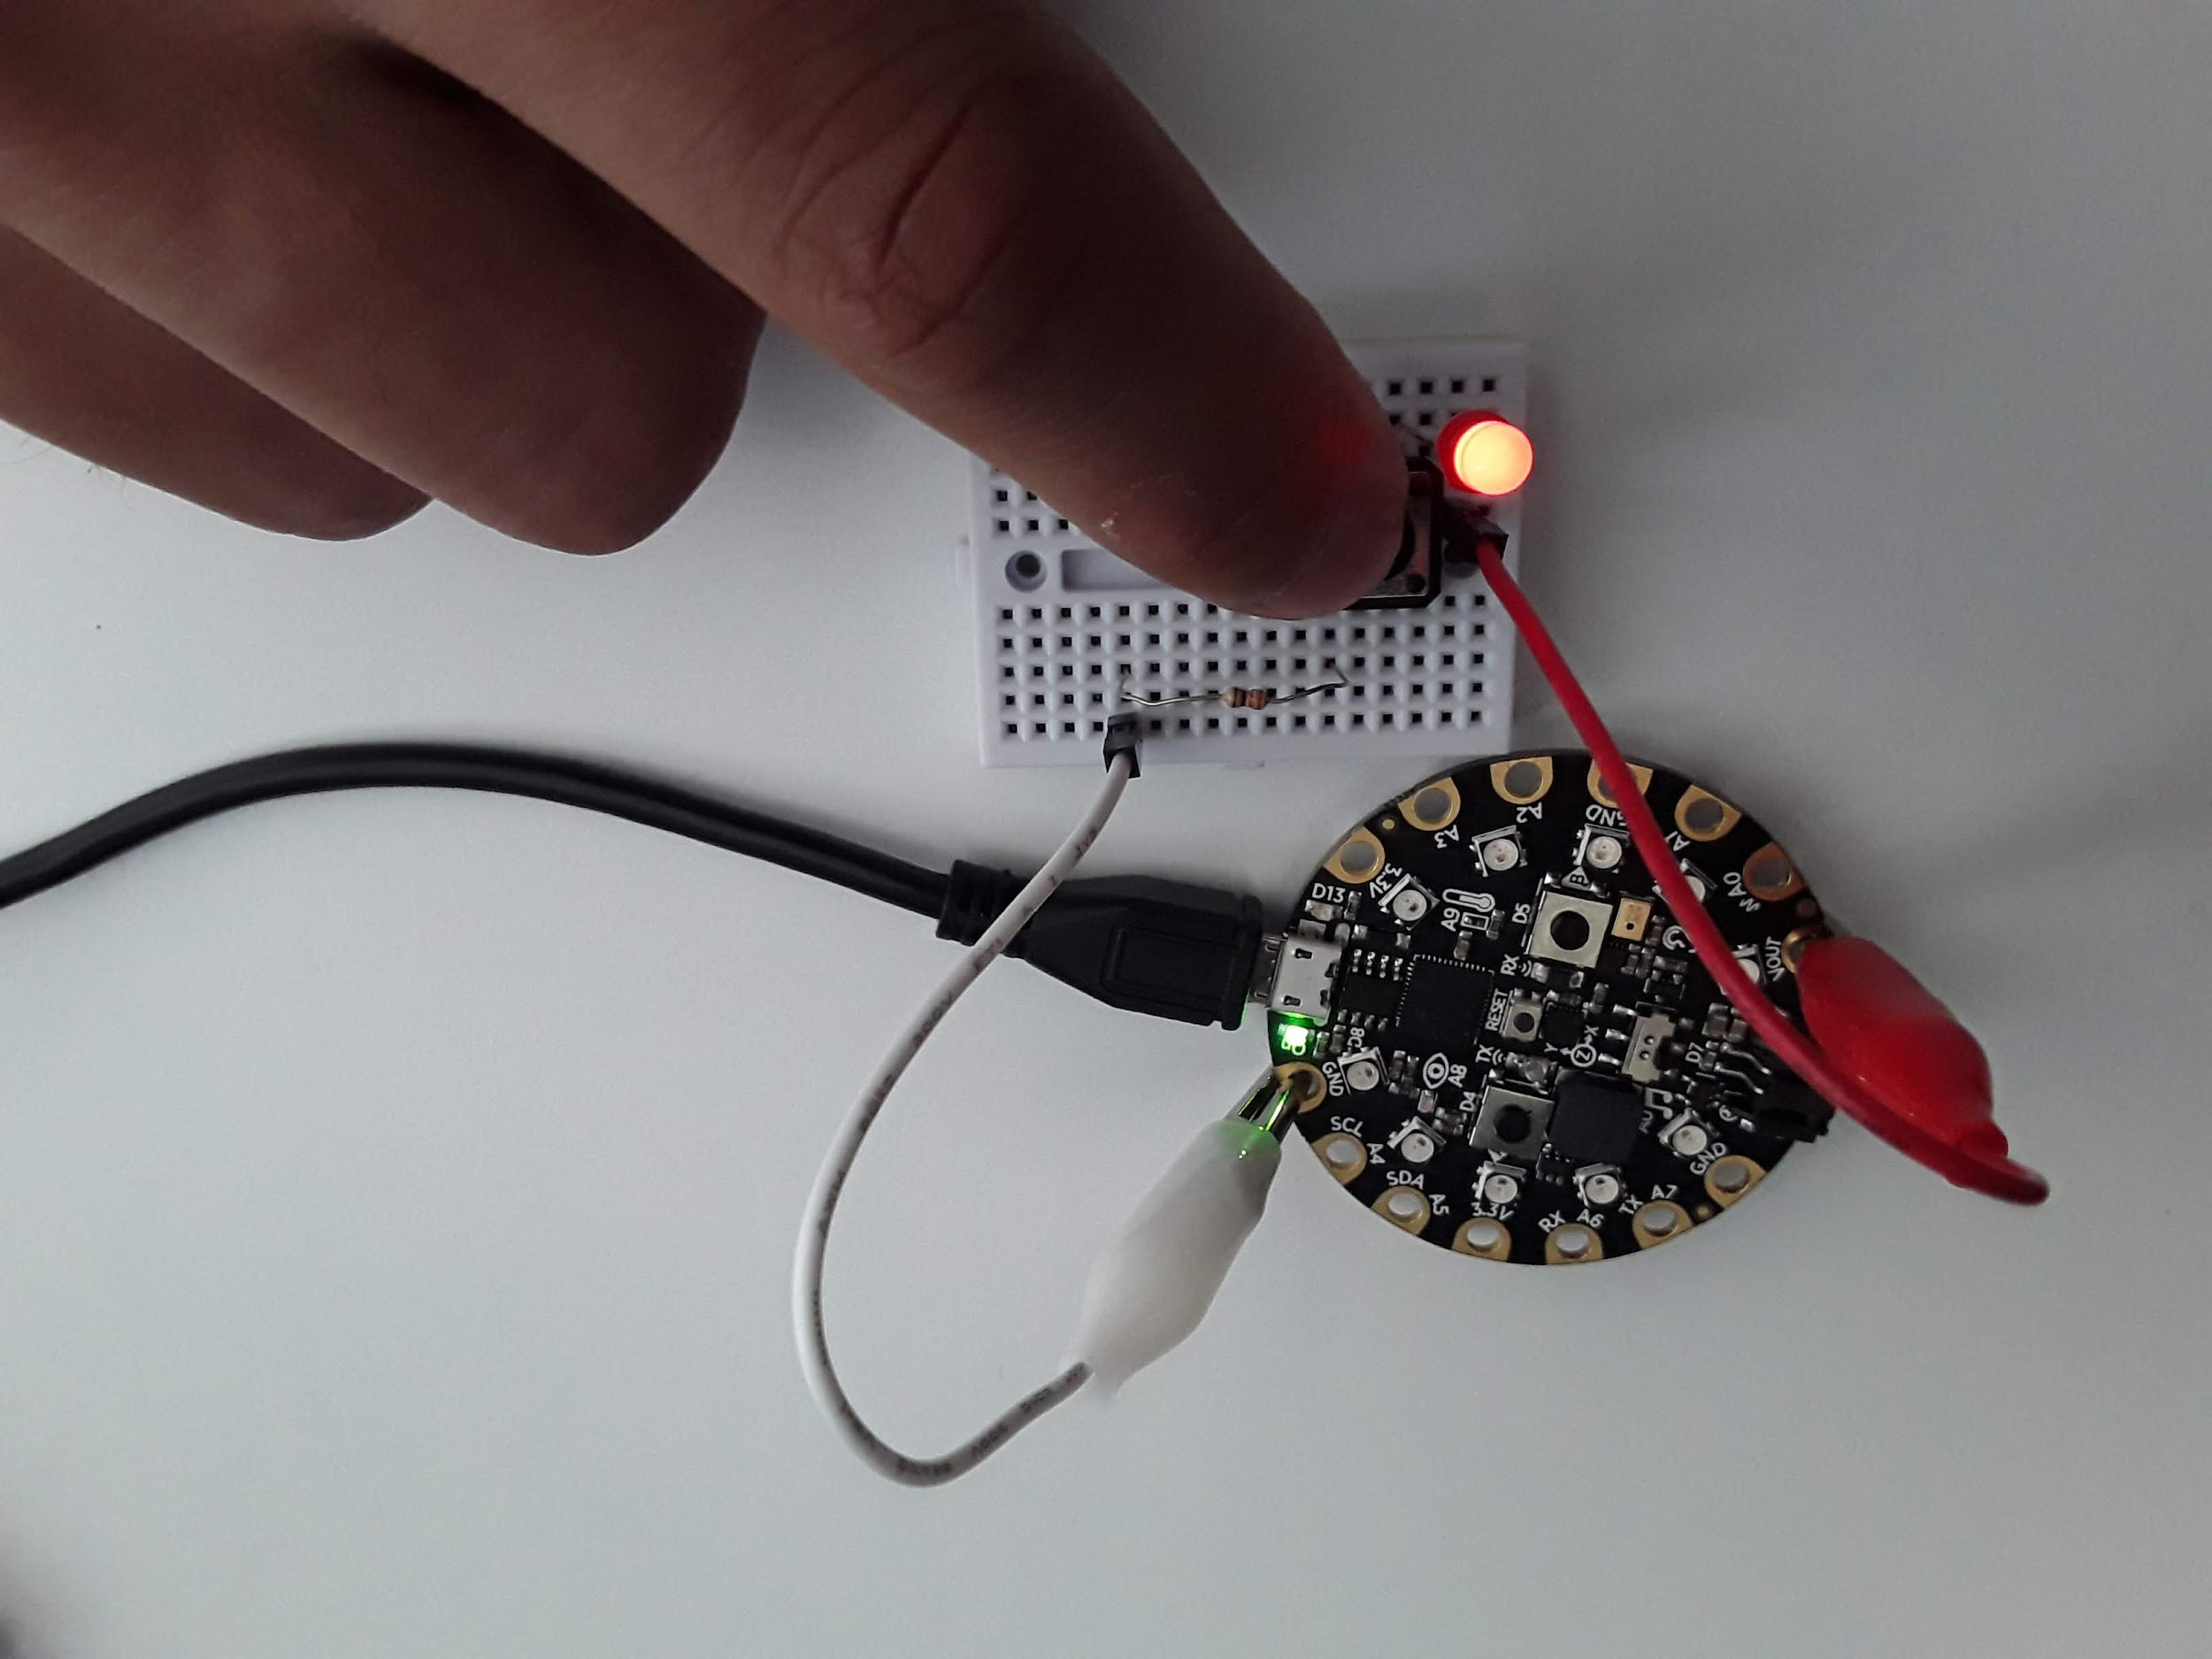
\includegraphics[width=\textwidth]{Figures/LED3.jpeg}
  \end{center}
\end{figure}

\subsection{LED with code}

Next I want you to remove the button from the circuit and wire up the
LED like you had it when the positive end was connected to VOUT or
3.3V. Except this time I want you to hook the positive end of the
circuit to pin A2. Then edit your blink code to blink pin A2. Take
a look at the blink 
code. Right now the code is blinking pin D13. How do you think you
need to change the code to blink pin A2? Here’s what my circuit looks
like for this one. I won’t include code for this one since you just
need to change one line of code.
\begin{figure}[H]
  \begin{center}
    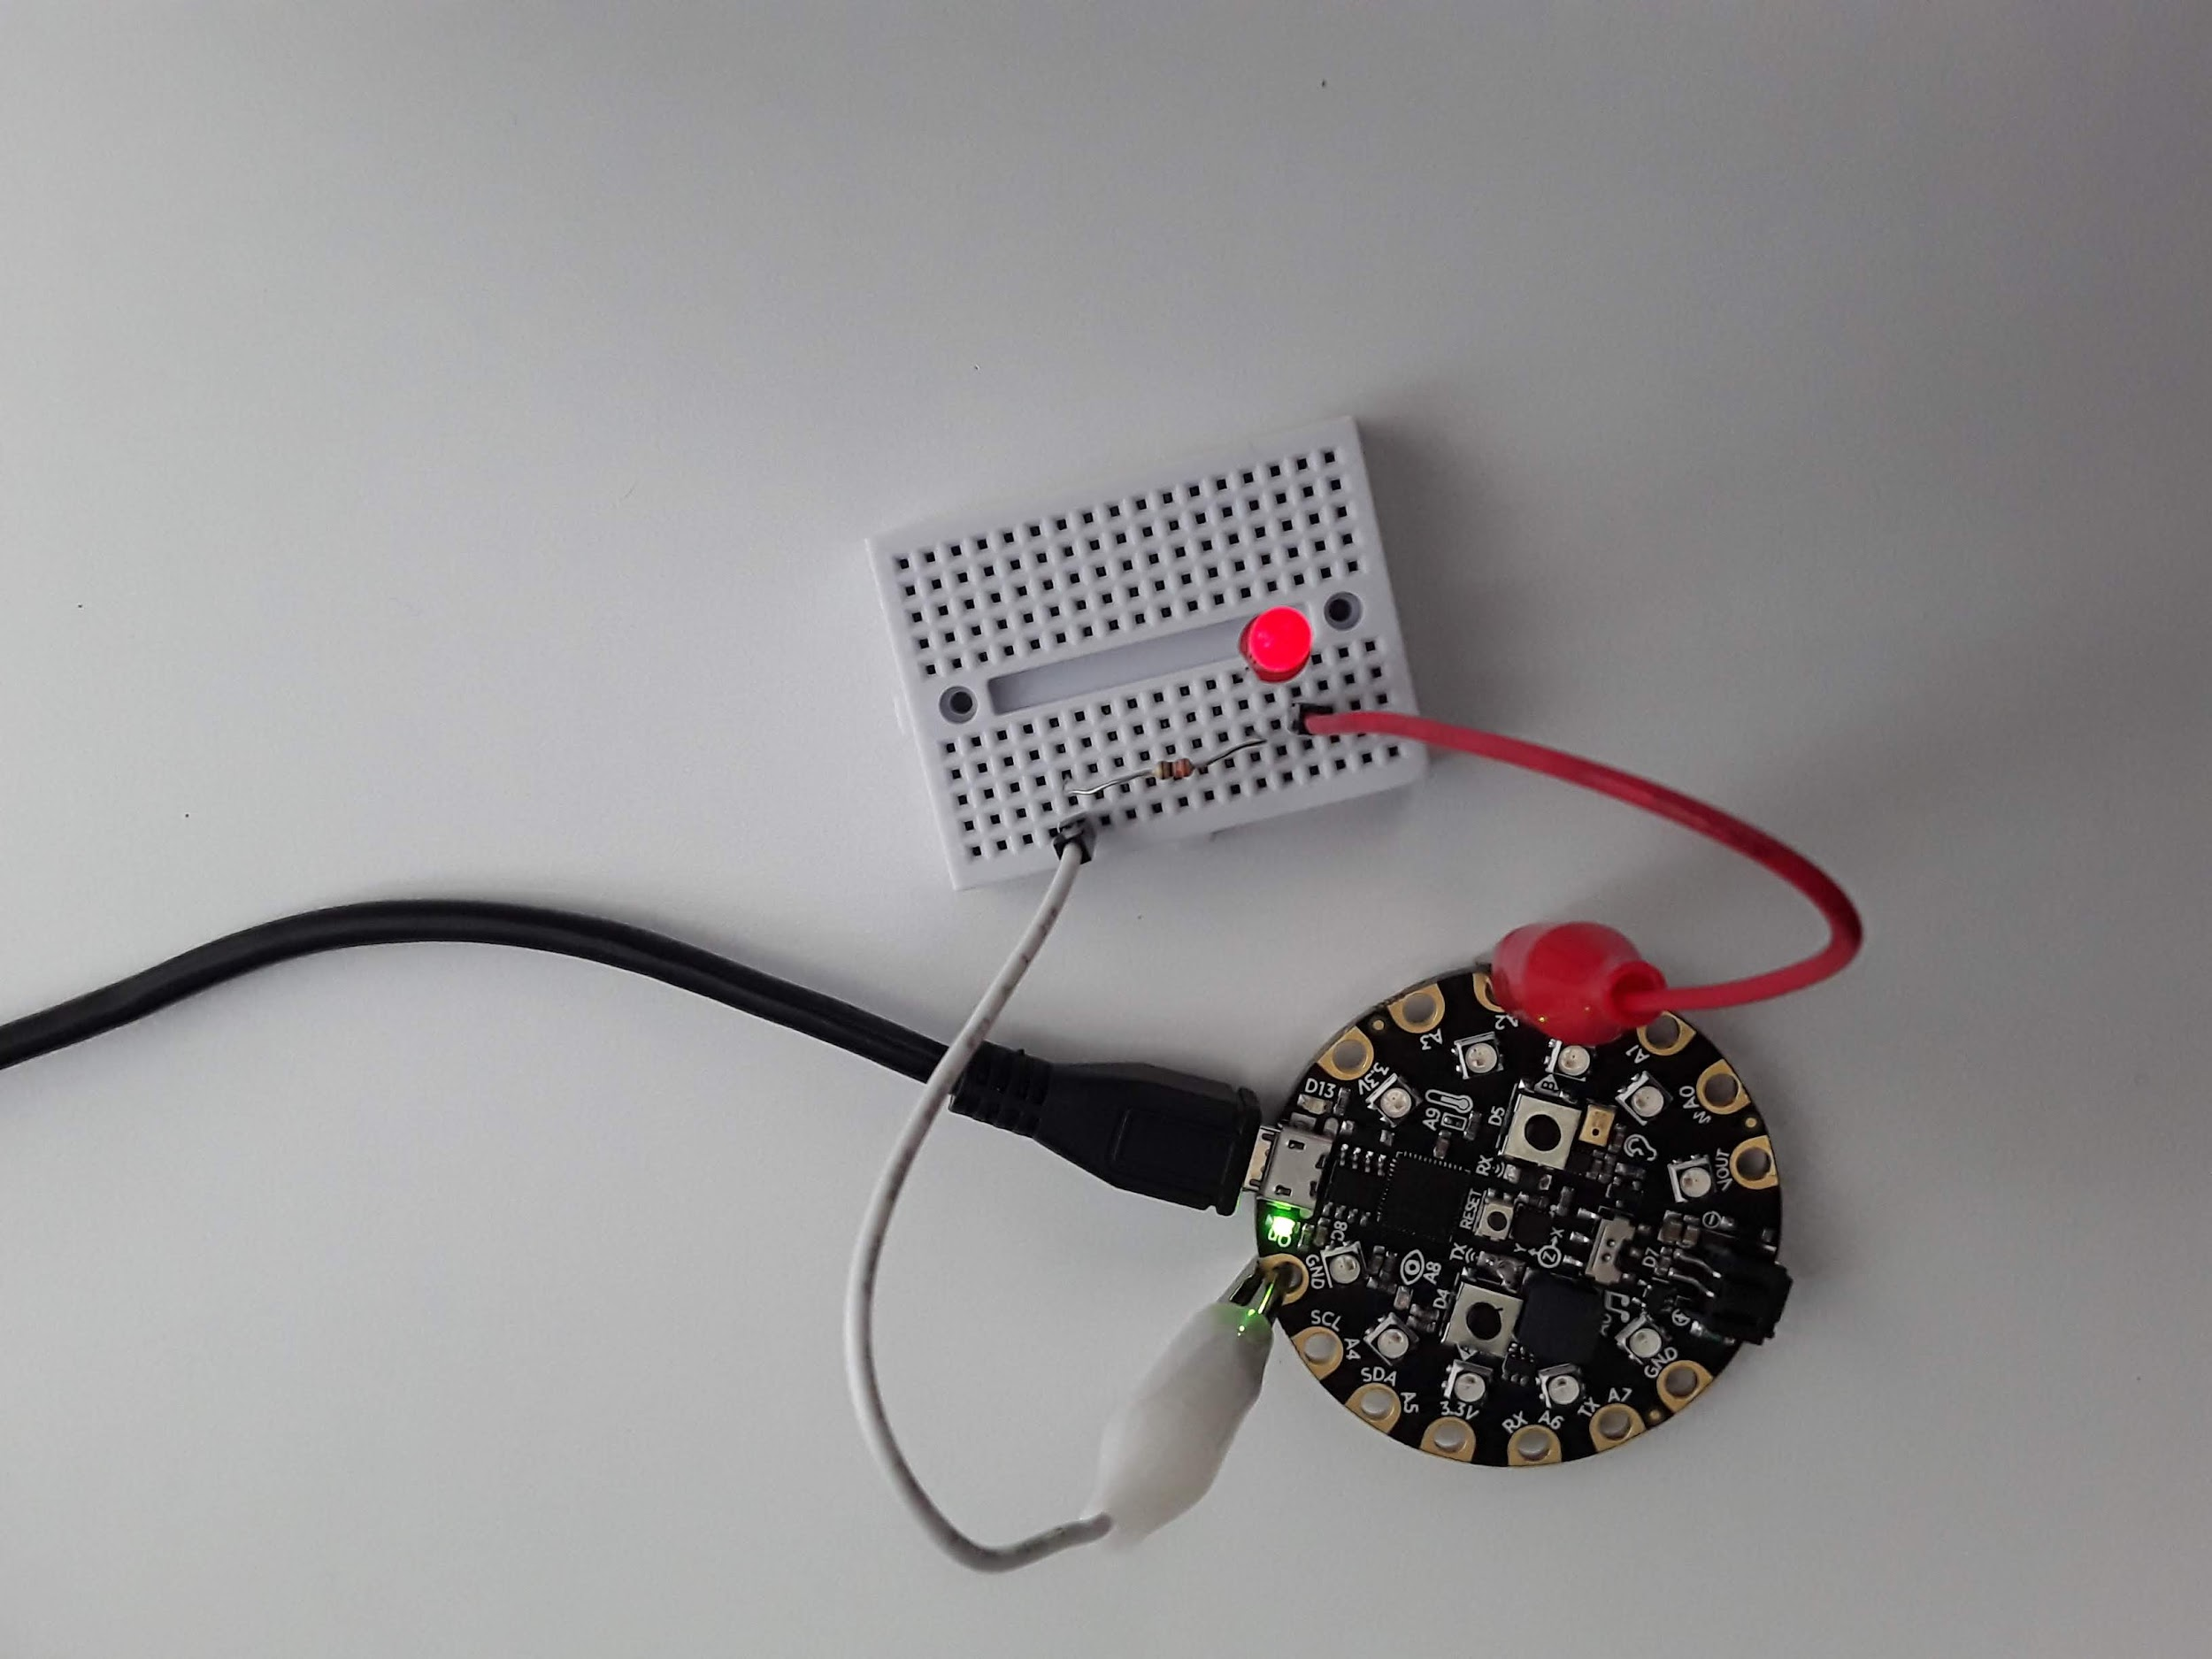
\includegraphics[width=\textwidth]{Figures/LED4.jpeg}
  \end{center}
\end{figure}

\subsection{LED with CPX button}

Finally, I want to use one of the buttons on the CPX to blink the LED
hooked up to pin A2. For this code to work you first need to detect a
button press and then tell the program to change the light from True
to False depending on what it’s current status is. This one is a bit
more difficult so I’ll include the code here and discuss the code
itself. Here is my circuit (identical) to the previous one with Button
A on the CPX pressed down. 
\begin{figure}[H]
  \begin{center}
    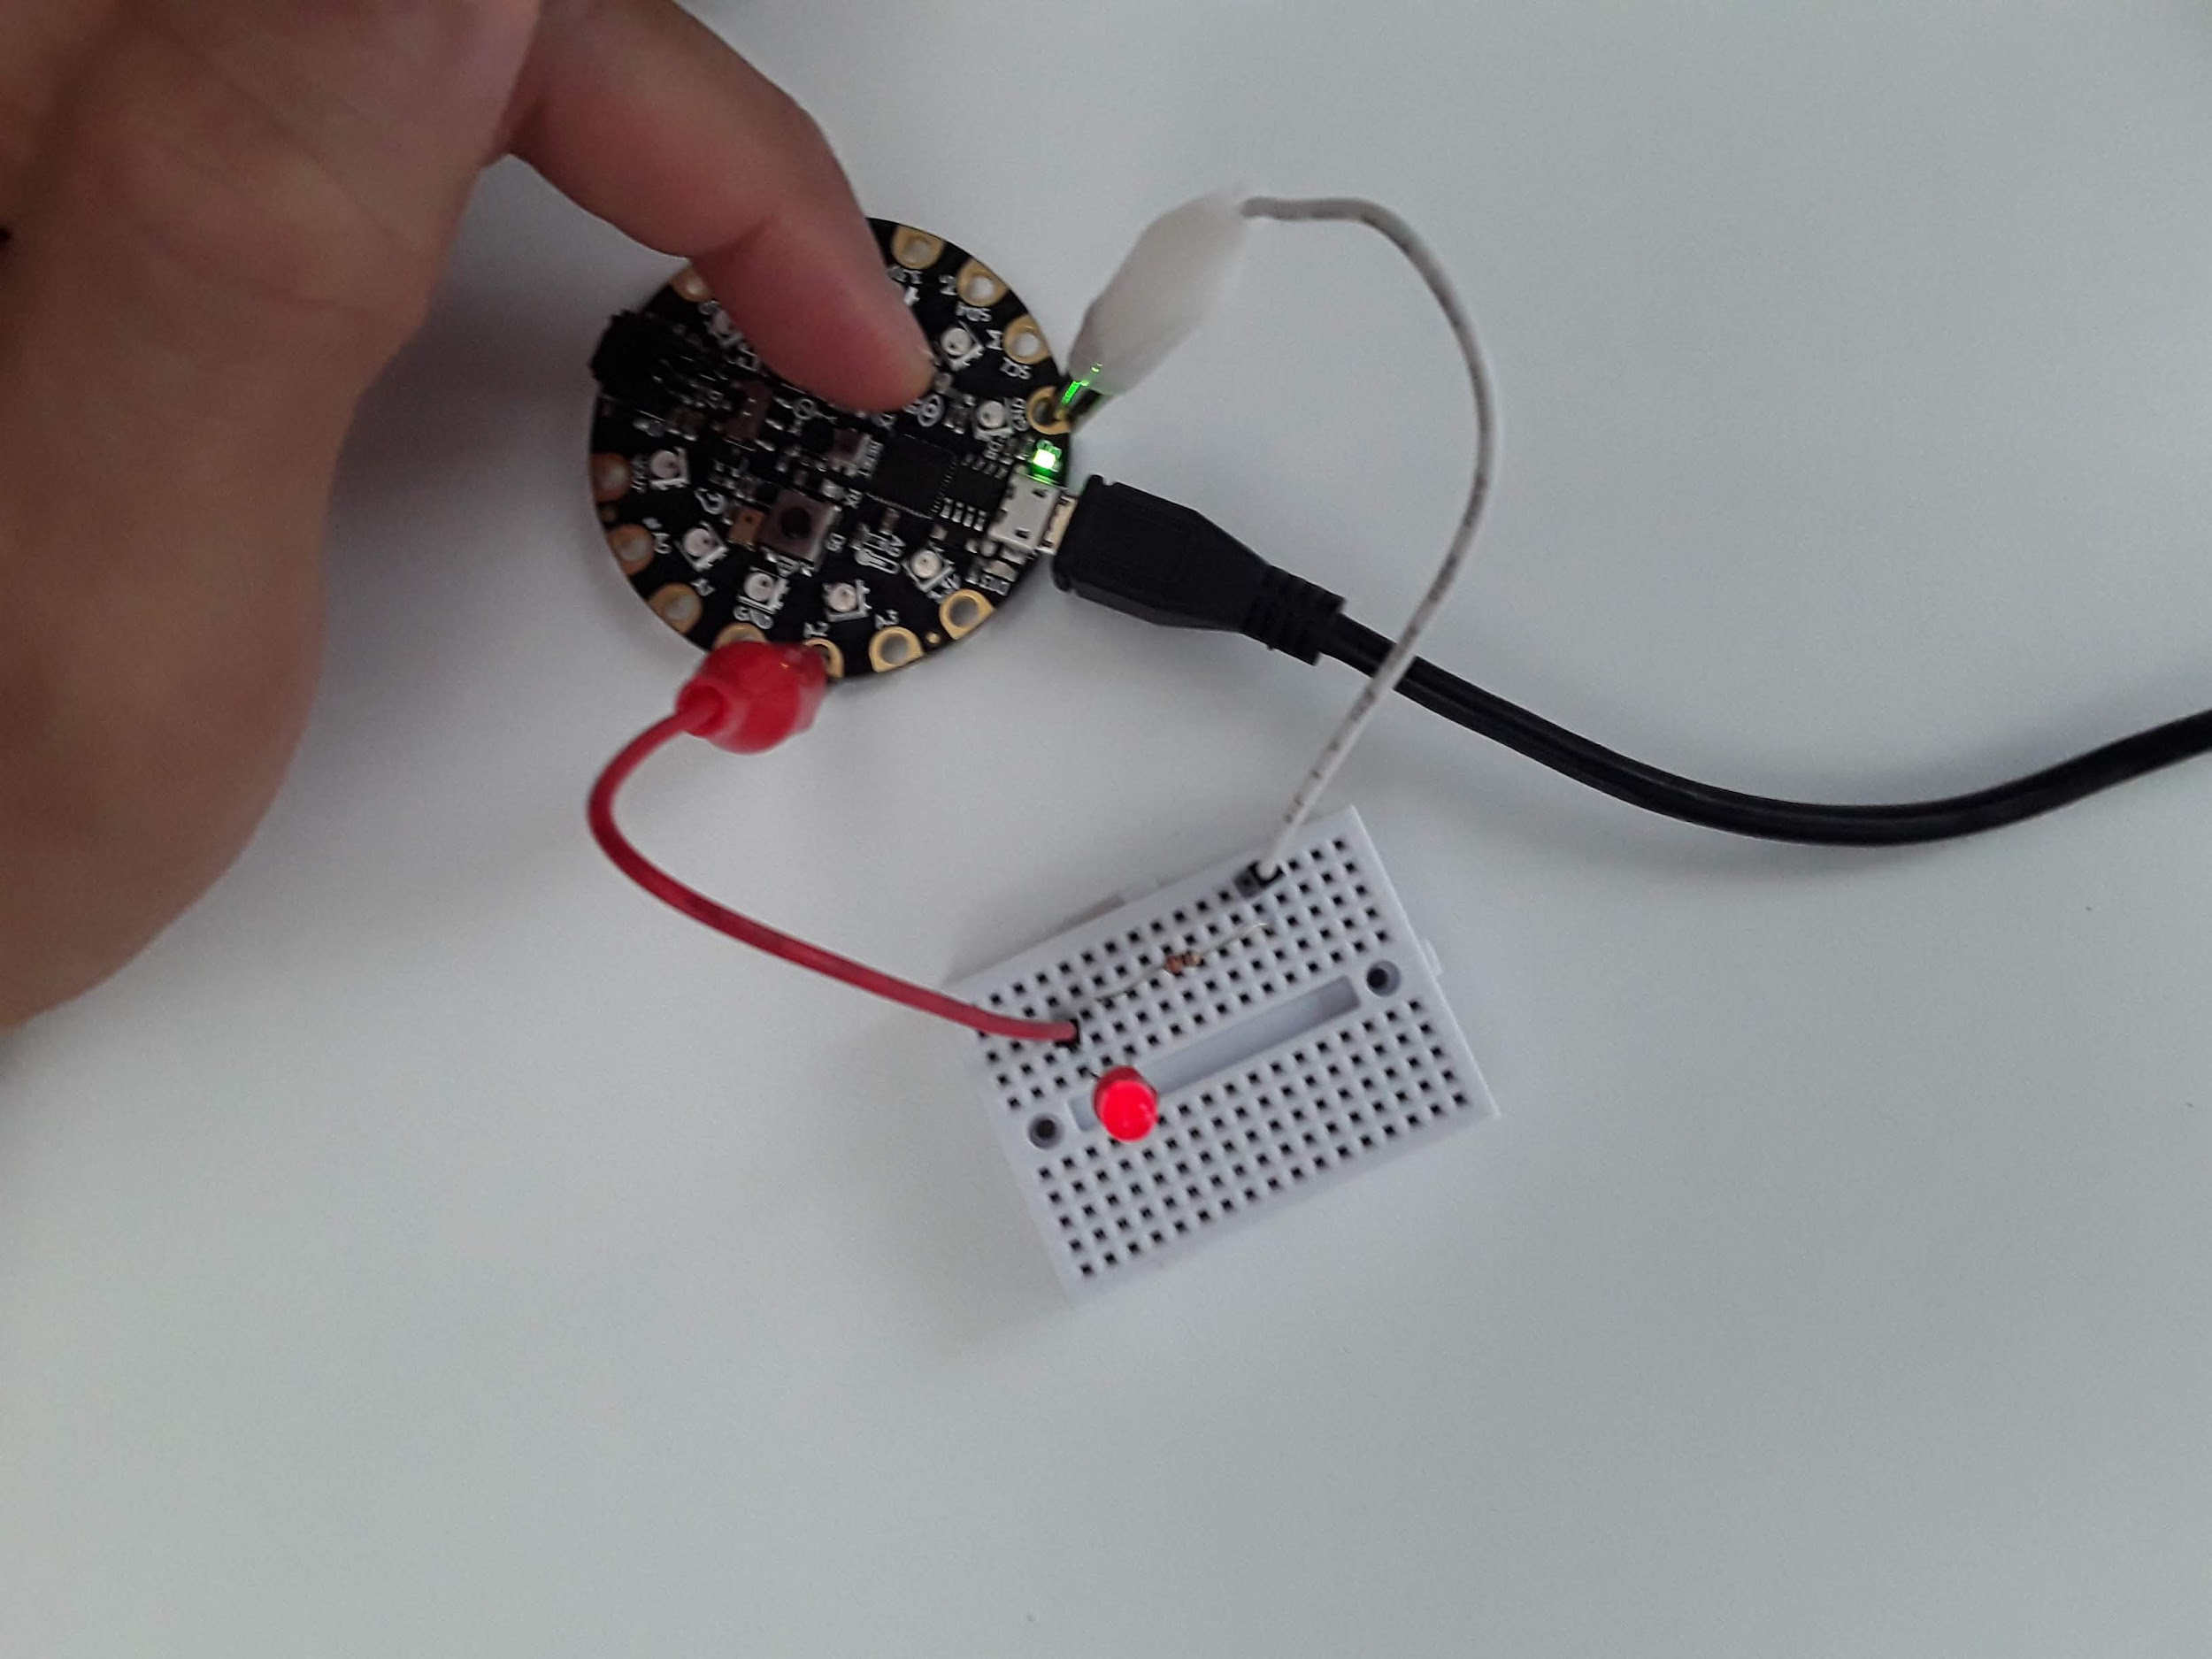
\includegraphics[width=\textwidth]{Figures/LED5.jpeg}
  \end{center}
\end{figure}
Alright so how do we detect a button press? Well the documentation on
this is not so straight forward. What we want to do is detect the
INPUT of a digital signal and then do something if we detect that
signal. Here’s the code I created to get it to work.
\begin{figure}[H]
  \begin{center}
    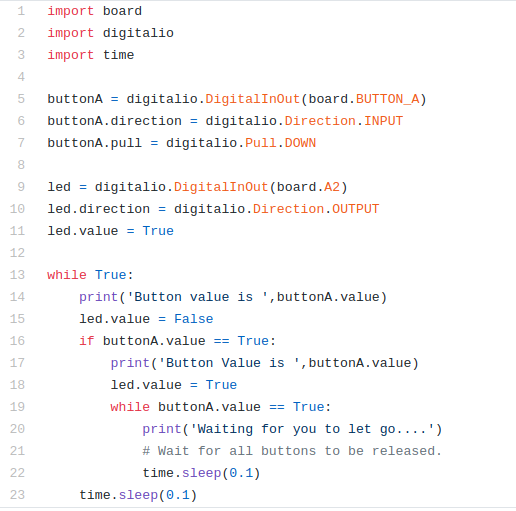
\includegraphics[width=\textwidth]{Figures/button_blink.png}
  \end{center}
\end{figure}
The code above is an image. You could type exactly what you see and
hope you don't type any errors (which is highly unlikely) or you could
look for my code on my
\href{https://github.com/cmontalvo251/Microcontrollers/tree/master/Circuit_Playground/CircuitPython}{Github}. Have
you bookmarked this link yet? I recommend you do so!!! So you're
making a code about Buttons....hmmm. Click that Github link. Where do
you think the code about Buttons is located? Anywho, let's talk about
the code.

The first 3 lines are exactly the same as before. Line 5 through 7 are
similar to creating the “led” variable except we’re using {\it BUTTON\_A} as
the board value and setting the direction to {\it INPUT}. Finally we’re
setting the pull direction to {\it DOWN}. This means the button acts like a
pull down resistor and when it’s pressed the value of the button goes
{\it HIGH}.

Lines 9-11 are the same as before. We create an led variable and tell
the CPX that the led is hooked up to pin A2. We then start the while
loop on line 13. First if you click the Serial button you’ll see the
text ‘Button value is False’. It’s False because {\it buttonA.value} is not
being pressed. On line 15 the led is set to False (turned off). On
line 16 the button value is checked using an if statement as to
whether or not the button is pressed (True). If the button is pressed,
the user will be notified that the button is pressed on line 17 and
the led will be set to True (on) in line 18. Lines 19-22 are while
loop that will notify the Serial monitor that you must let go of the
button before the code can continue to the main while loop. The
{\it time.sleep} functions are there to make sure a human can operate the
button without code running faster than a human can press a
button. When I press the button down here is the output I get from the
{\it Serial} monitor. 
\begin{figure}[H]
  \begin{center}
    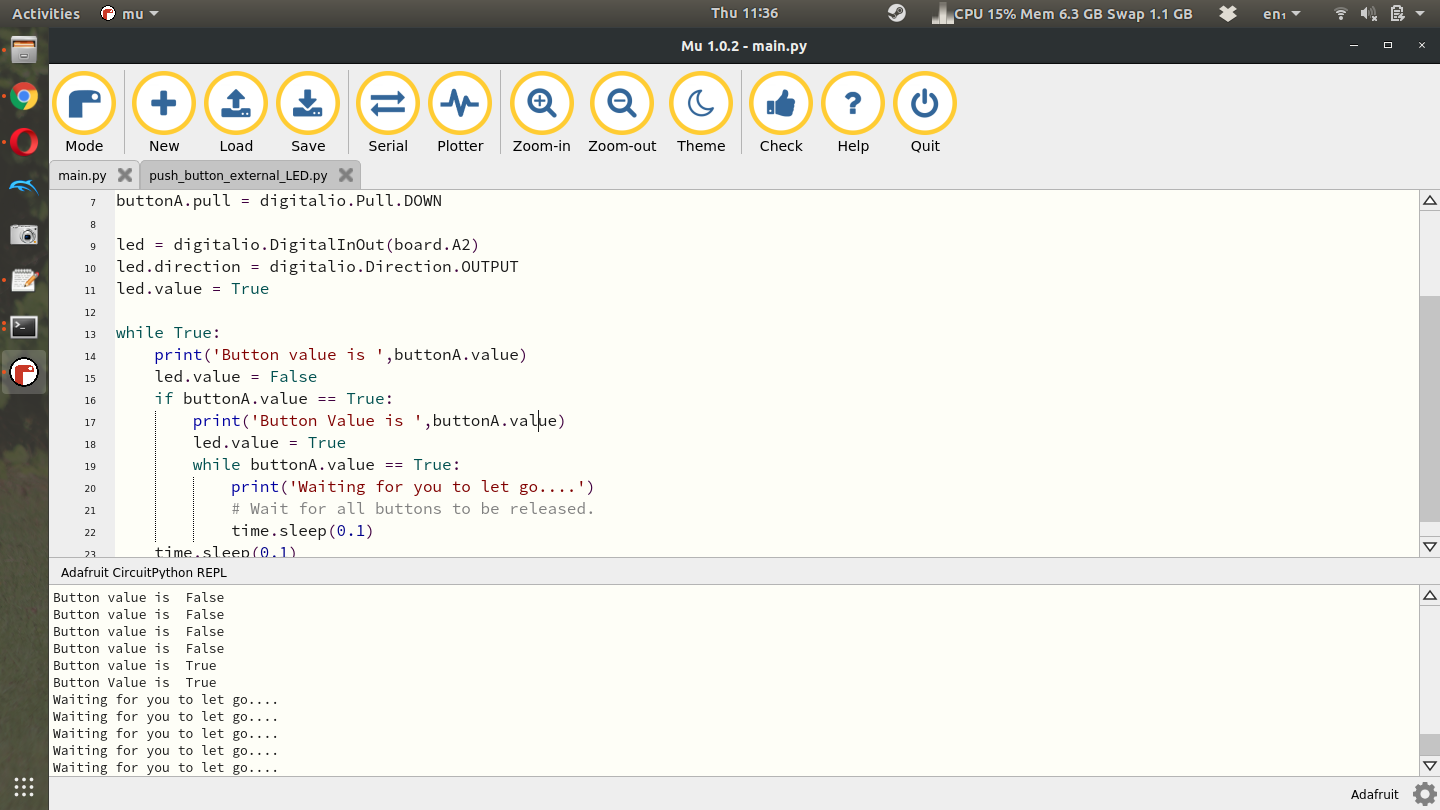
\includegraphics[width=\textwidth]{Figures/MuButton.png}
  \end{center}
\end{figure}
Here you’ll see 4 lines that say ``Button value is False" and then two
lines that say ``Button value is True" followed by 5 lines that say
``Waiting for you to let go...". See if you can get this code to work and
play with it and modify it as you see fit. By the way, the LED
connected to pin D13 has this exact same circuitry, an LED a resistor,
it’s all just soldered to the PCB so you don’t have to build it using
a breadboard. Hopefully now you have some appreciation for buttons and
LEDs!! 

\subsection{Assignment}

Once you've completed the project above, upload a PDF with all of the photos and text
below included. My recommendation is for you to create a Word document
and insert all the photos and text into the document. Then export the
Word document to a PDF. For videos I suggest uploading the videos to
Google Drive, turn on link sharing and include a link in your
PDF. Note that all code must be included in the appendix or you'll be
penalized 10\%. 


\begin{enumerate}[itemsep=-5pt]
\item Include a photo of your circuit with your LED turned on using VOUT (make sure your face is in the photo) - 20\%
\item Include a photo of your circuit with your LED turned on using 3.3V (make sure your face is in the photo) - 20\%
\item Include a video of you turning your LED on and off with the push button (again make sure your face is in the video for enough time to say who you are and say hello) - 20\%
\item Include a video of your LED blinking on and off automatically by modifying the blink code (make sure your face is in the video for enough time to say who you are and say hello) - 20\%
\item Include a video of your LED blinking by pressing a button on the CPX. Note the LED must blink while you press and hold the button. You'll need to modify the code to get that to work. (make sure your face is in the video for enough time to say who you are and say hello) - 20\%
\end{enumerate}


\section{Using the CPX/CPB as a Data Acquisition System (DAQ)}
\label{s:daq}

\subsection{Parts List}

\begin{enumerate}[itemsep=-5pt]
\item Laptop
\item CPX/CPB
\item USB Cable
\end{enumerate}

\subsection{Learning Objectives}
\begin{enumerate}[itemsep=-5pt]
\item Record real time measurements from the CircuitPlayground using the Serial monitor
\item Learn how to use the typing module to type data directly into a spreadsheet or text file
\item Learn how to log data on the on board memory of the CircuitPlayground 
\end{enumerate}

\subsection{Extra Help}

This is a pretty hard project to do with multiple different
methods. After you’ve read through this document I suggest you watch
a youtube I created on \href{https://youtu.be/yX0zeIfn2j4}{Logging Data with the Circuit Playground
Express}. I have also made video where I \href{https://www.youtube.com/watch?v=Vc7_KxRnORI}{log temperature and
accelerometer data using on board memory with the CircuitPlayground
Bluefruit.}

\subsection{Getting Started}

Taking data is the core of any instrumentation project. Data
Acquisition Systems or DAQ for short come in all shapes and
sizes. Believe it or not the CPX can be used as a crude and cheap
DAQ. The CPX can easily take temperature data and monitor the
temperature in a greenhouse or take humidity readings of a plant to
monitor soil content. Before we learn about the different sensors on
board the CPX, we want to make sure we can store that data later
rather than just having it spit data out via the serial monitor. For
starters though let’s get the CPX to print out something simple like
button presses since we’ve touched on that already. The code I’m using
is shown below and can also be found on
\href{https://github.com/cmontalvo251/Microcontrollers/blob/master/Circuit_Playground/CircuitPython/Data_Logging/button_presses.py}{Github}.
\begin{figure}[H]
  \begin{center}
    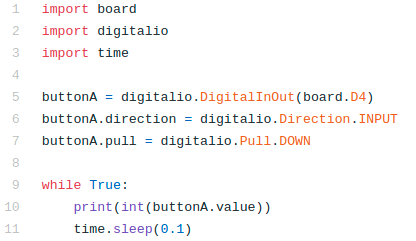
\includegraphics[width=\textwidth]{Figures/button_presses.png}
  \end{center}
\end{figure}
The code is pretty similar to what I had in the past. I import board,
digitalio, and time. I create a buttonA object using the digitalio
library to record button presses. I then enter into a while loop print
the buttonA.value. The difference here is that I use the int()
function to convert the buttonA.value to an integer. The reason why I
do this is because buttonA.value is a boolean. It is either True or
False. An integer though is a number and thus a value of False is 0
and True is 1. If you open the serial monitor and push the A button
down a few times you’ll see some zeros and 1’s.
\begin{figure}[H]
  \begin{center}
    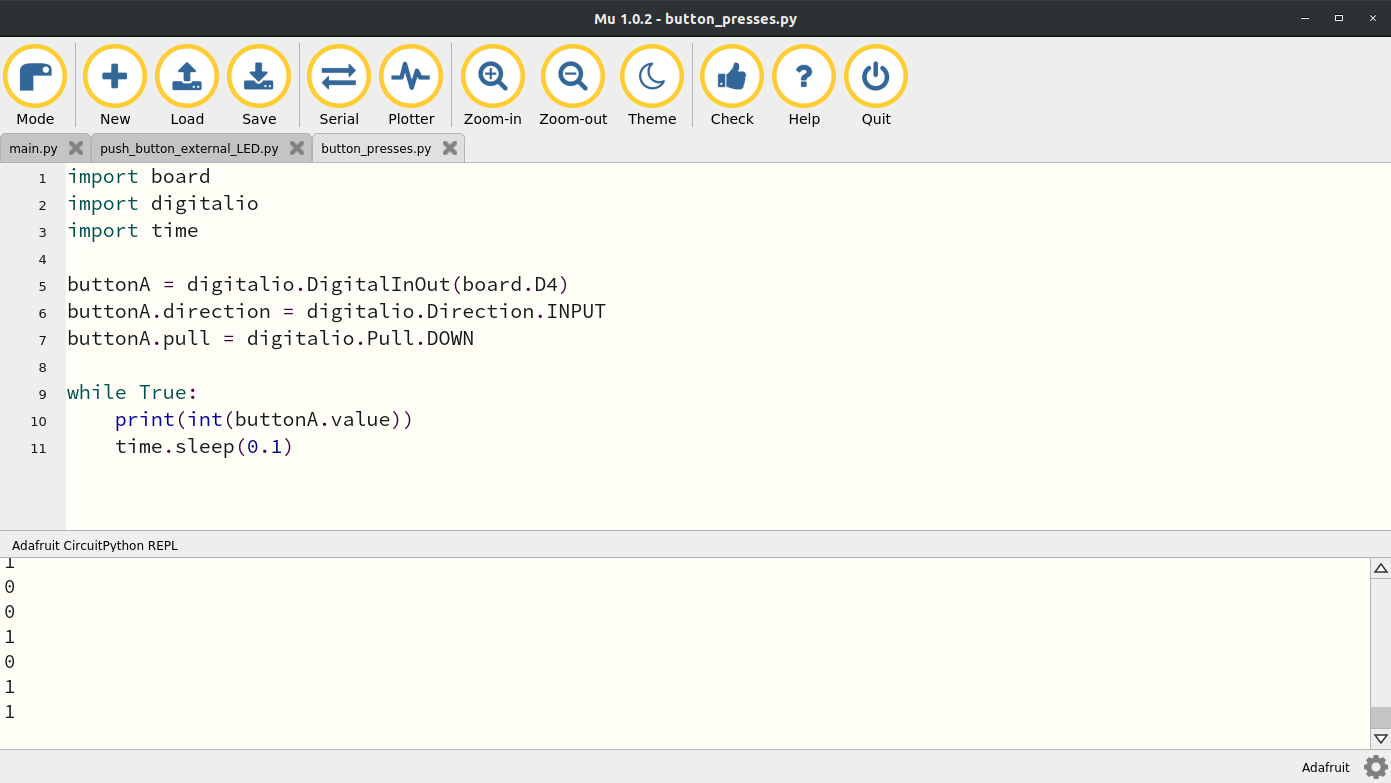
\includegraphics[width=\textwidth]{Figures/MuButtonPress.png}
  \end{center}
\end{figure}
Mu also has a really neat builtin plotter. You’ll see next to the
Serial button there is a button called Plotter. If you click that
button now nothing will pop up on the screen. Unfortunately in order
to plot using the Plotter you need to modify the print() statement to
this:
\begin{verbatim}
print((int(buttonA.value),))
\end{verbatim}
Notice the extra parentheses and the comma. Now if you click Plotter
you’ll see something like this. You’ll notice that the print statement
now has commas in it and the Plotter is recording button presses. 
\begin{figure}[H]
  \begin{center}
    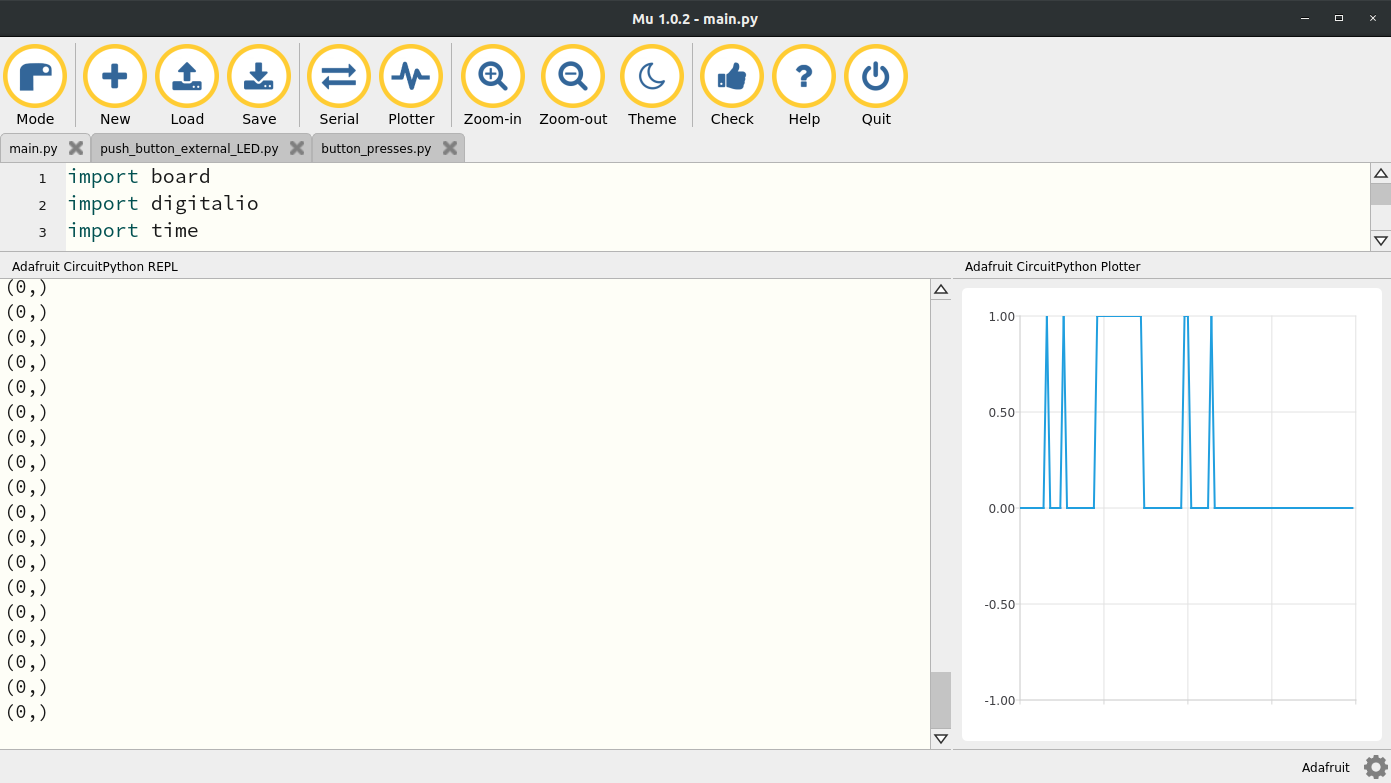
\includegraphics[width=\textwidth]{Figures/MuPlotter.png}
  \end{center}
\end{figure}
The problem with this is we still can’t save the recorded data
anywhere. Before we get into saving data let’s first edit the print
statement again to get rid of the Plotter by removing the extra
parentheses and add time.monotonic() that way we can keep track of
when a button was pressed. My print statement looks like this now: 
\begin{verbatim}
print(time.monotonic(),int(buttonA.value))
\end{verbatim}
Looking at the serial monitor now you’ll see that time is being
printed alongside the button presses. 
\begin{figure}[H]
  \begin{center}
    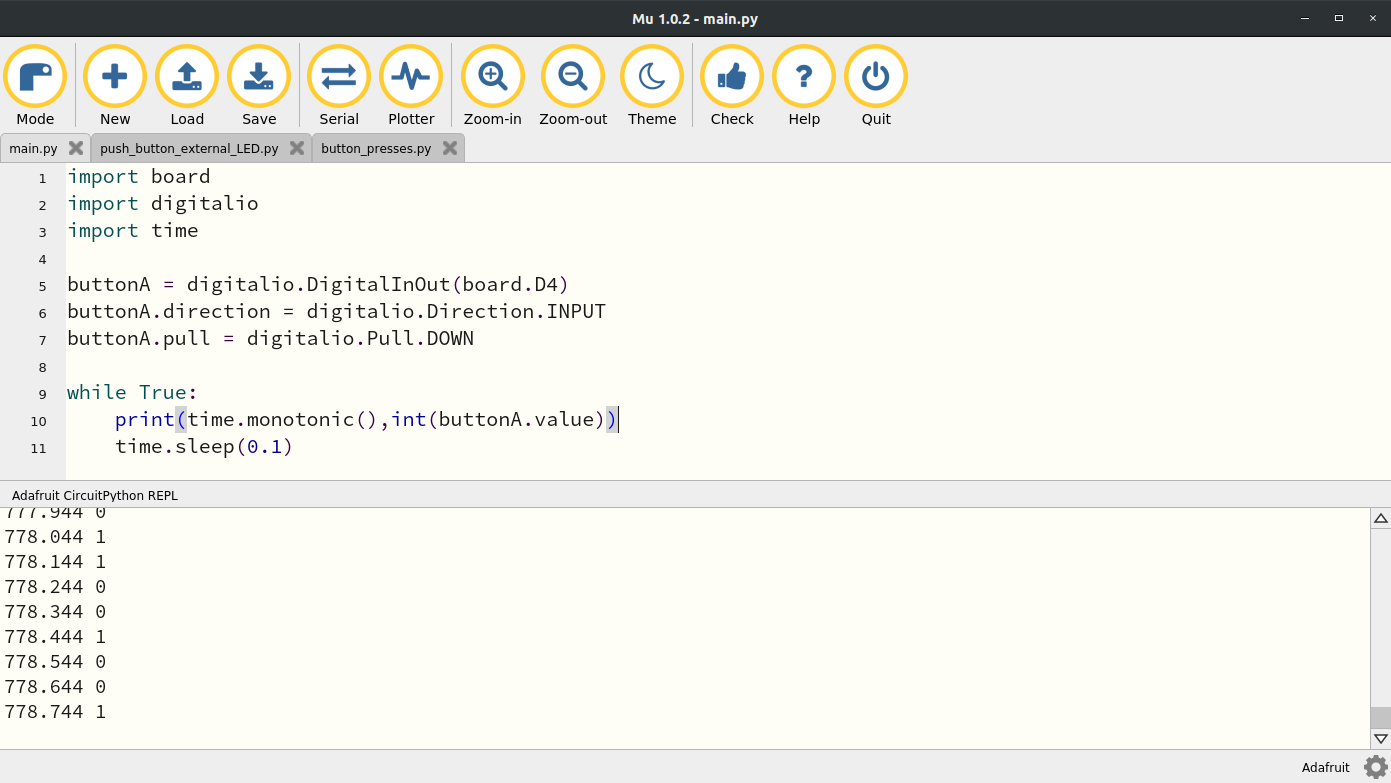
\includegraphics[width=\textwidth]{Figures/MuPlotterTime.png}
  \end{center}
\end{figure}
Now we are in a position where we can record some data and save it to
our computer. There are 3 ways to record data. I call the first,
Method1 and you basically just copy and paste from the serial monitor,
Method2 where you have the CPX/CPB type data into a spreadsheet and
Method3 where you log data internally onto the CPX/CPB itself.

\subsection{Method 1 - Copying Serial Monitor Data}

If you open up the serial monitor you can see the data output. If you
unplug the CPX while it’s taking data the code will stop. {\bf Note: In
newer versions, unplugging your CPX will result in a loss of data. If
this happens try pressing CTRL+C after you click the REPL window.} With
the code stopped you can select all the data in the Serial monitor and
then copy and paste the data into a text file on your computer. You
can actually copy this into a new file on Thonny and just save it as a
*.txt file. Once you have the data in a text file you can proceed to
plotting in Python on your desktop which I discuss in the last
section.Here’s some example data in Gedit which is a simple text
editing program.
\begin{figure}[H]
  \begin{center}
    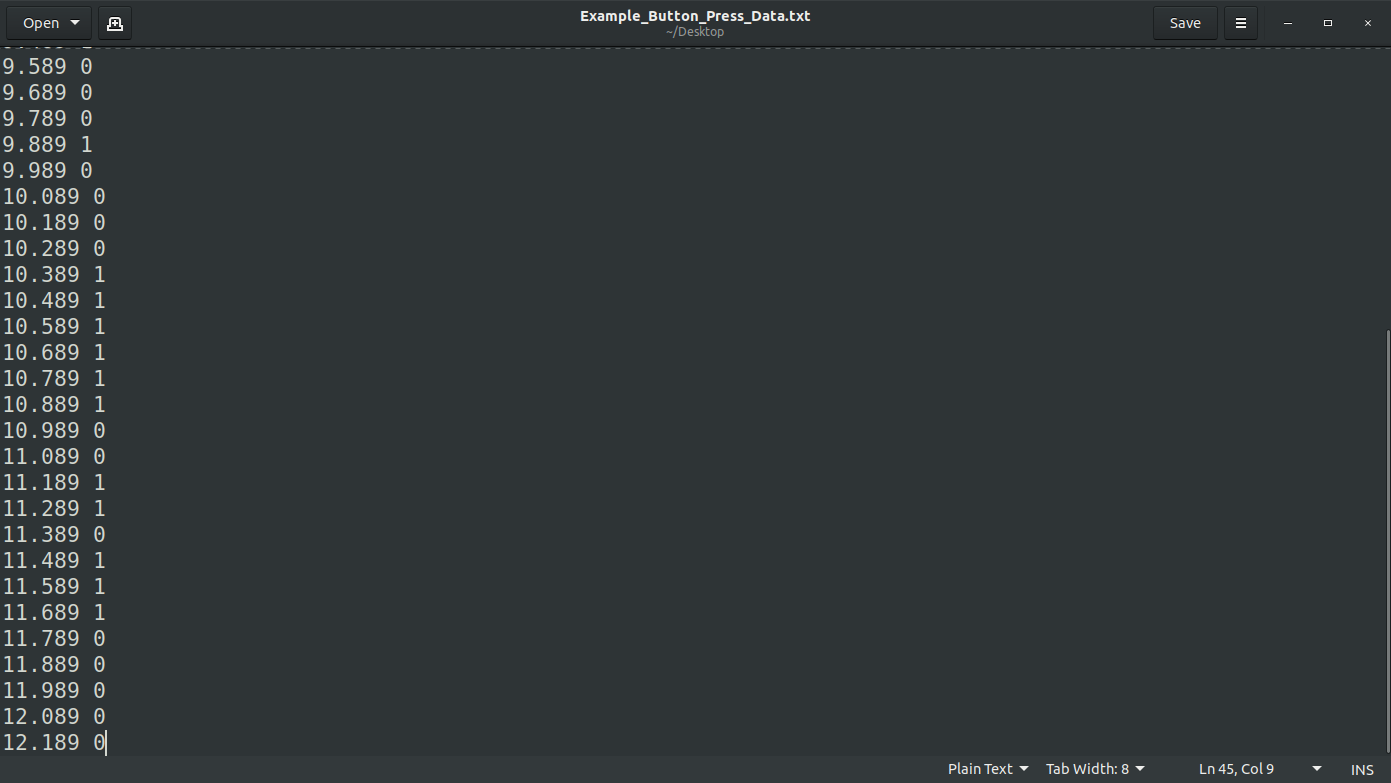
\includegraphics[width=\textwidth]{Figures/Gedit_Data.png}
  \end{center}
\end{figure}

\subsection{Method 2 - Automatically Populate a Spreadsheet}

The downside with the above method of course is if you have a ton of
data to record you could lose the data or run into a massive copy and
paste issue. The second option is to use this module called keyboard
which takes control of your keyboard on your desktop computer and
actively types your data into a spreadsheet. The code is very
extensive but I’ll include the simple one here so we can discuss
it. Below are the first 30 lines of code. The first 6 lines of code
are just comments since I heavily adopted this code from the \href{https://learn.adafruit.com/make-it-a-keyboard/circuitpython}{Adafruit
Learn System}. \href{https://github.com/cmontalvo251/Microcontrollers/blob/master/Circuit_Playground/CircuitPython/Data_Logging/record_button_presses_typing.py}{My version of this code} can be found on my Github. Lines 8 -
14 are import commands as we’ve seen previously. The regular import
modules board, time and digitalio are imported but we are also
importing the Keyboard module so that the CPX can takeover our
keyboard. Lines 16-22 create two buttons. First we create buttonA
attached to pin D4 and then a switch attached to pin D7. If you look
on the CPX there is a switch labeled D7. Before you copy this code
onto the CPX make sure you move the switch towards the ear looking
symbol. Lines 26-28 created the keyboard object. We are going to call
it layout for this example code.
\begin{figure}[H]
  \begin{center}
    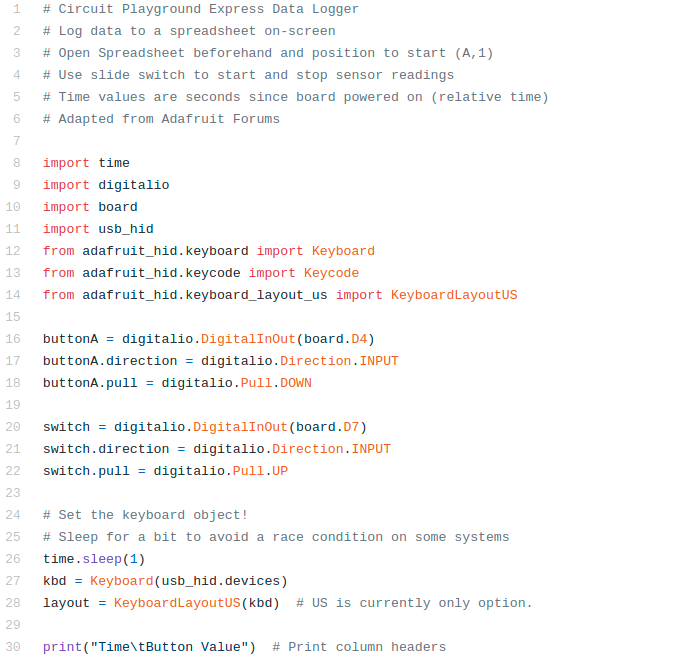
\includegraphics[width=\textwidth]{Figures/Typing1.png}
  \end{center}
\end{figure}
The next 30 lines are shown below. Lines 32-35 define a
function. Functions in Python have a pretty standard structure. The
keyword def is used to denote that the next line is a definition for a
function. The name of the function is {\it slow\_write()}. The input to the
function is string which ironically enough is a string object. Line
33-35 define what the function does. Line 33 sets up a for loop where
the code loops through each character in the string. Everytime it gets
to a new character it will use your keyboard to type that character
using the layout.write(c) command. The time.sleep(0.02) is just to
slow down the keyboard so your computer can keep up. That function is
defined above the standard while True: statement on line 37 but is
called on line 42. You’ll see there is a {\it slow\_write(output)} on line
42. In this case output is a string and it’s sent to the function
{\it slow\_write()}. So in this case we have a function that can write a
string so we just need to take data and then write it using our
keyboard. Line 38 is an if statement that will only be true if the
switch on pin D7 is pushed towards the music note on the CPX. If the
switch is not thrown the code will move to the else statement on line
52 and tell the user that you need to flip the switch. If the switch
is thrown line 40 will take data for us. First it will record the
time.monotonic() and store it as a floating point number using the
\%0.1f designation which means that it will store 1 decimal as a
\%floating point number for f.
\begin{figure}[H]
  \begin{center}
    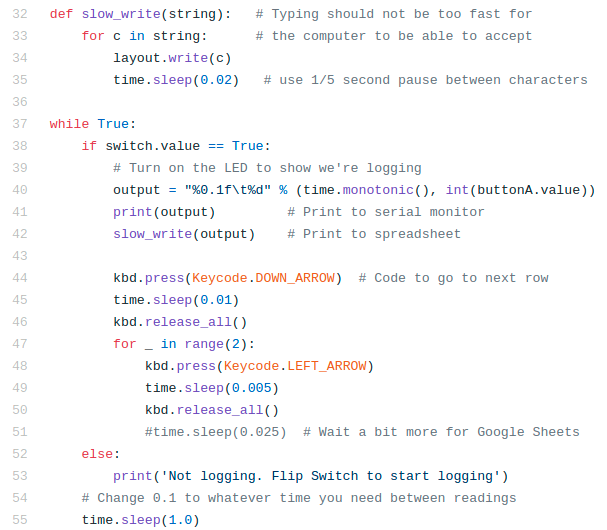
\includegraphics[width=\textwidth]{Figures/Typing2.png}
  \end{center}
\end{figure}
The second number in the string is an integer or a base 10 (decimal)
integer designated by the \%d part of the format. The integer is
int(buttonA.value). You’ll see a \t in between the formatted numbers
which is a tab. The tab is there to tab between cells in a
spreadsheet. Line 41 will print the output string to the Serial
monitor and it will also type the contents of the string. Very
important here. When you flip the switch on the CPX your keyboard will
start typing in whatever active window is selected. If you don’t have
a spreadsheet opened and active (selected), the keyboard will just
begin typing in whatever window is open. Make sure you have a
spreadsheet program open and ready to go. Lines 44-51 tell the
keyboard to hit the {\it DOWN\_ARROW} on your keyboard to move to the next
row and the {\it LEFT\_ARROW} twice to move back to the first column. Line 55
is a sleep to only log data once a second. I ran this code for a bit
and had it type into LibreOffice Calc which is a free spreadsheet
program. Google Sheets or Microsoft Excel will also work just fine. 
\begin{figure}[H]
  \begin{center}
    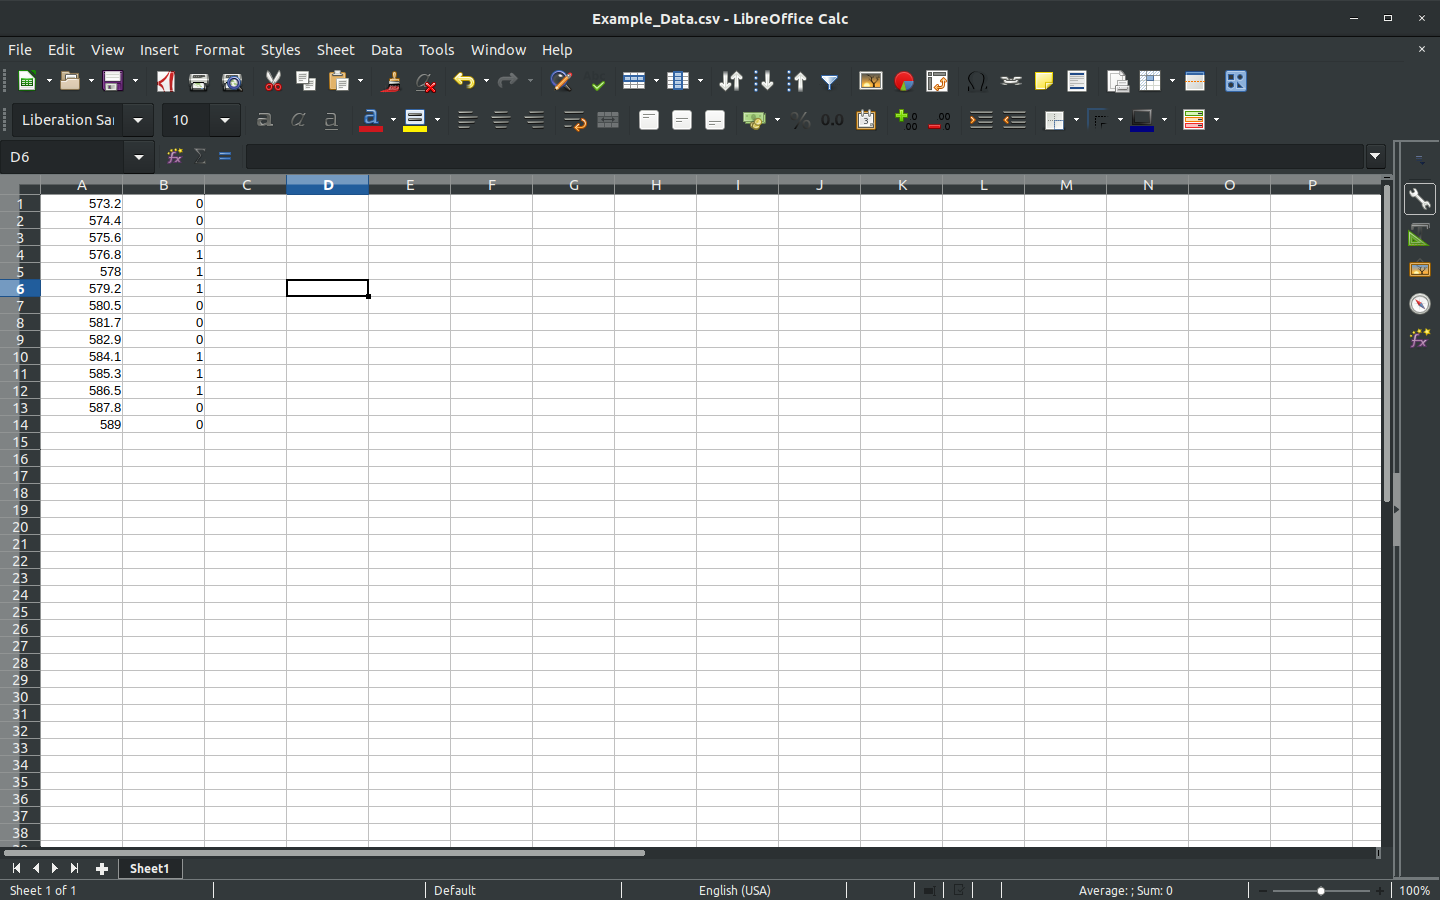
\includegraphics[width=\textwidth]{Figures/Typing3.png}
  \end{center}
\end{figure}
You’ll see that the first column is time with 1 decimal point and the
second column is the button press values. At this point you must click
{\it Save As...} and save the document as a CSV which stands for Comma
Separated Value. Once you have the file saved you can proceed to
plotting in Python on your Desktop. 

\subsection{Method 3 - Logging Data Directly to on board memory}

The problem with the above 2 methods is that you need a laptop to log
data in the field. It would be nice if you could use the optional
battery pack and just have the CPX log data on the CPX itself. This is
the most complex way but in my opinion the best way. In order to get
this to work you need to allow the drive on the CPX to have read/write
permissions. This requires you to load a piece of software called
boot.py and put it on the CPX. I have this
\href{https://github.com/cmontalvo251/Microcontrollers/blob/master/Circuit_Playground/CircuitPython/Data_Logging/boot.py}{software
  on my Github}. The software is shown below. The first 10 lines are
probably very familiar. Import some modules and then create a switch object. Line 13
is where all of the storage permissions are changed. If the flip is
switched towards the A button, the storage module is used to allow you
to write to the CPX. The problem here is that if you do this, you
won’t be able to edit code. I’ll explain the procedure here in a
minute. As always, the relevant Adafruit tutorial is on the \href{https://learn.adafruit.com/adafruit-circuit-playground-express/circuitpython-storage}{Adafruit
Learn System} if you want to read more about it. Again make sure you
store this file onto the CIRCUITPY drive and save it as boot.py
\begin{figure}[H]
  \begin{center}
    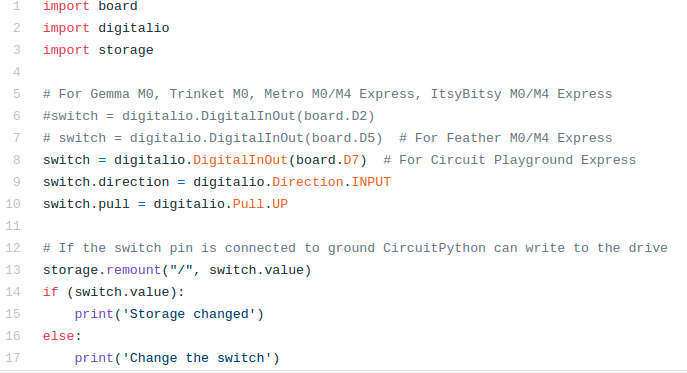
\includegraphics[width=\textwidth]{Figures/boot.png}
  \end{center}
\end{figure}
In addition to storing the file boot.py you’ll need to edit your
main.py script to only log data when the switch is moved towards the B
button. The software to record button presses on disk is shown below
and as always
\href{https://github.com/cmontalvo251/Microcontrollers/blob/master/Circuit_Playground/CircuitPython/Data_Logging/write_button_presses_disk.py}{on
  my Github}. In this software we again see the standard 
commands. Lines 1-3 import all the modules we need and then 5-15
create a switch, a button and an LED. In this case we’re using the LED
soldered to the board. Line 17-20 check to see if the user has flipped
the switch. If the switch is False the storage module on boot.py will
allow the drive to act like a data logger and it will open a file
called {\it Test\_Data.txt} for writing (‘w’). If the switch is True then the
user will be notified that the file has not been opened for
writing. Lines 22 through 33 include the infinite while loop. Line 23
turns the LED on and line 24 prints out the current time and the
button value in integer form. If the switch value is False the program
will create an output string by converting all numbers to strings
using the str function. Notice that there is a {\it
  str(``\textbackslash n")} at the end of
the output variable which tells the computer to write a new line of
data to the file. Lines 28 and 29 write the output to the file from
line 18 and then flush the output which means the CPX waits for the
data to be fully written before moving on. It also turns the LED off
so we know the CPX took data even when we aren’t looking at the Serial
monitor. If the switch value is true it means that the we never opened
the data file and thus we tell the user we aren’t logging data and
it’s time to flip the switch and hit reset. 
\begin{figure}[H]
  \begin{center}
    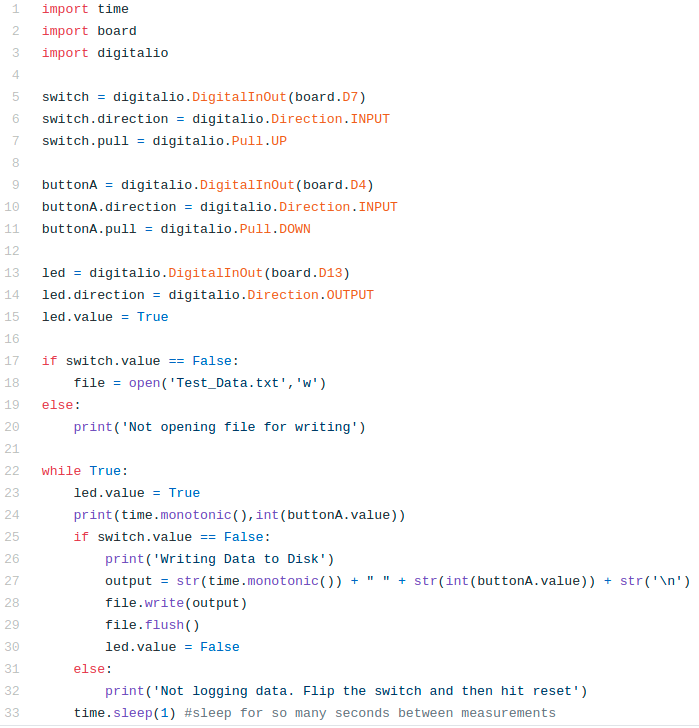
\includegraphics[width=\textwidth]{Figures/method3_1.png}
  \end{center}
\end{figure}
So here is the flow of what you want to do for method 3.
\begin{enumerate}[itemsep=-5pt]
\item Unplug the CPX
\item Flip the switch towards the A button.
\item Plug in the CPX and save the boot.py and main.py files. Remember you can only save Python scripts when the switch is flipped towards the A button.
\item When you are ready to start recording data, flip the switch towards the B button. If you’re looking at the Serial monitor, the software will throw an error. Just ignore it and hit the reset button. When your computer recognizes the CPX you can turn the Serial monitor on and off.
\item When you are done taking data simply slide the switch over towards the A button and hit reset again. This is what my Serial monitor looks like when I do this. You’ll see that I was writing to disk for like 25 seconds and then I flipped the switch back towards the A button.
\end{enumerate}
\begin{figure}[H]
  \begin{center}
    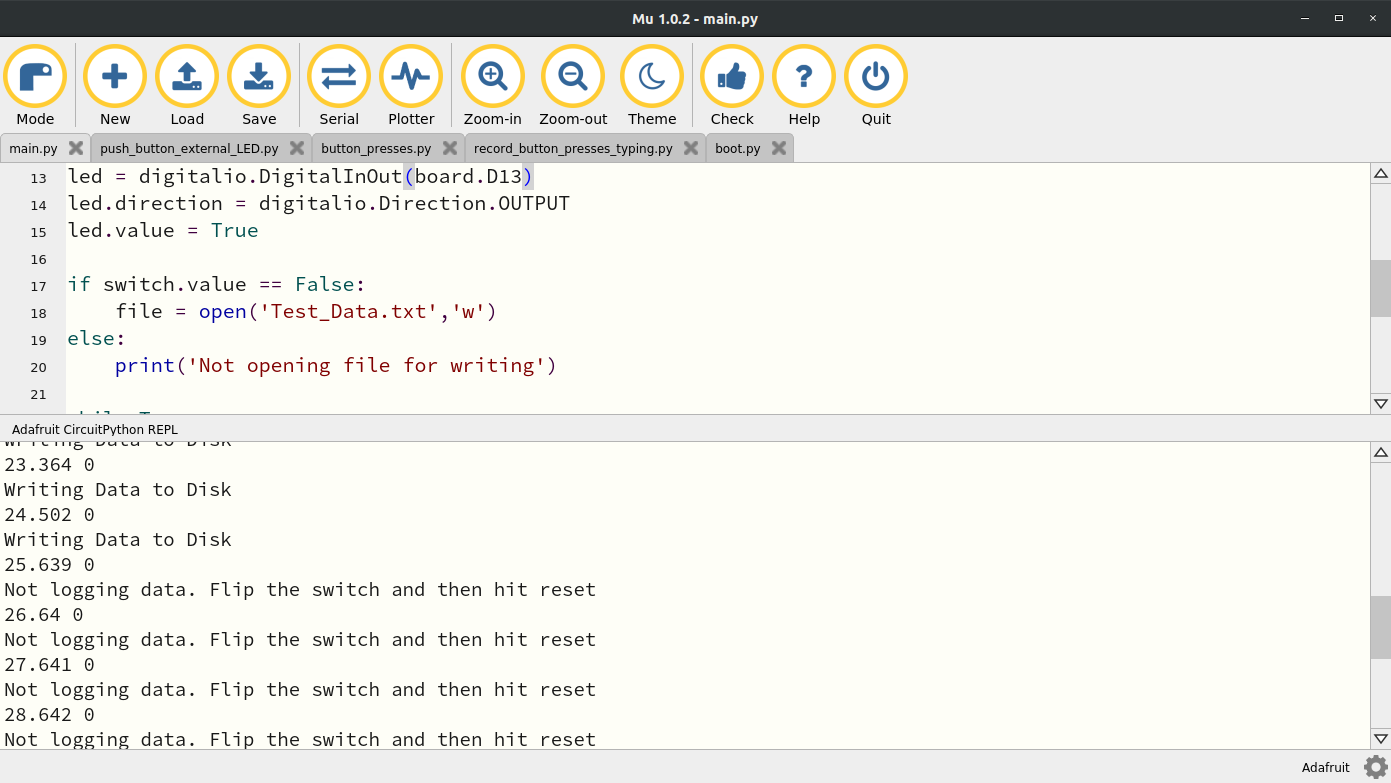
\includegraphics[width=\textwidth]{Figures/method3_2.png}
  \end{center}
\end{figure}
With the switch flipped and data taken, open your folder manager and
take a look at the CIRCUITPY drive. This is what mine looks
like. You’ll see I have two Python files and a file {\it Test\_Data.txt} with
all my data in it. 
\begin{figure}[H]
  \begin{center}
    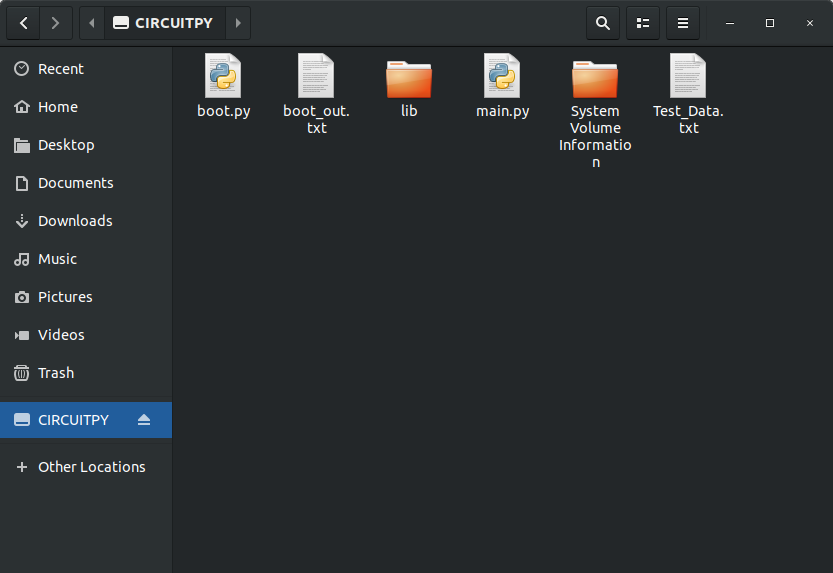
\includegraphics[width=\textwidth]{Figures/method3_3.png}
  \end{center}
\end{figure}
If you open the {\it Test\_Data.txt} file you will hopefully see data in it.
\begin{figure}[H]
  \begin{center}
    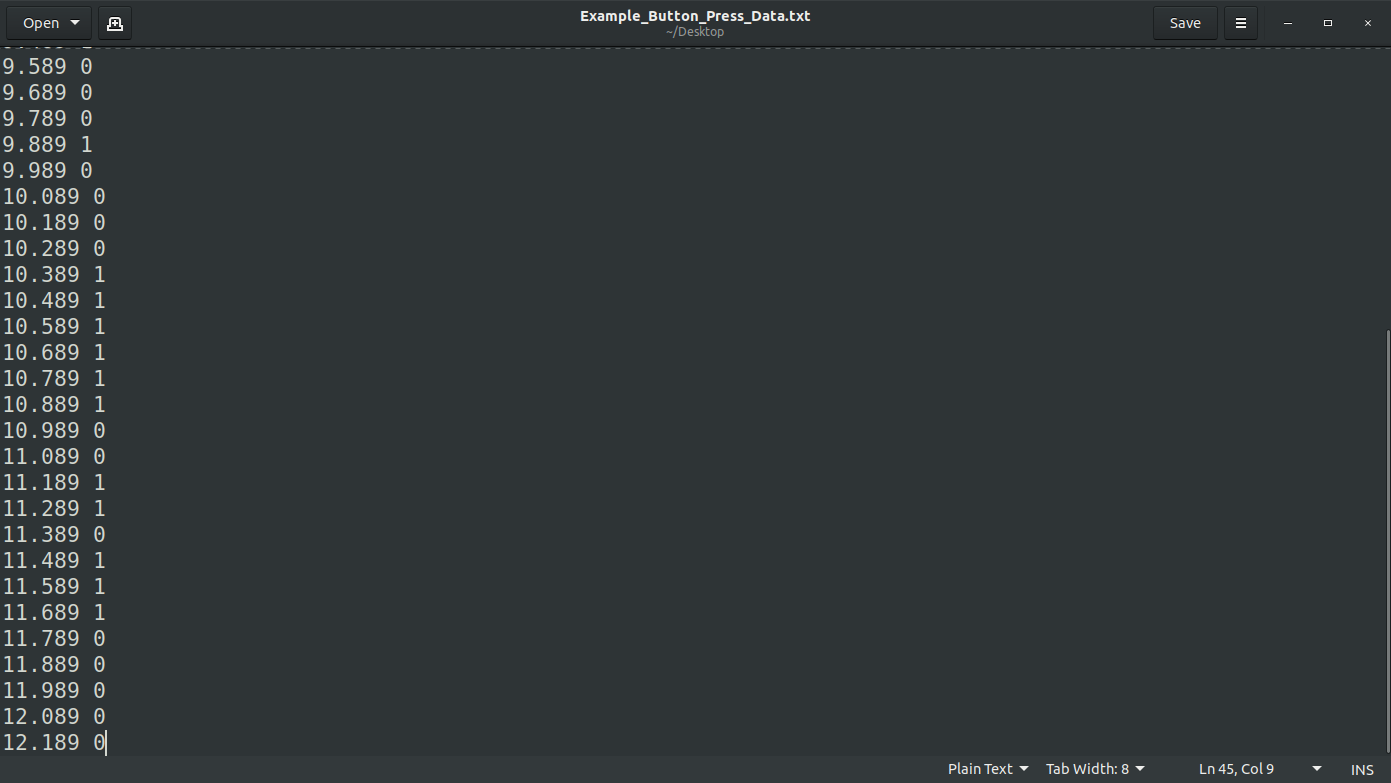
\includegraphics[width=\textwidth]{Figures/Gedit_Data.png}
  \end{center}
\end{figure}
At this point you can copy this text file over to your desktop computer and proceed to the Python plotting portion.
Ok so let’s recap method 3 one more time.
\begin{enumerate}[itemsep=-5pt]
\item Unplug CPX (or remove power)
\item Slide switch to A
\item Plug in CPX (or provide battery power)
\item Slide switch to B
\item Reset
\item Take data for however long you want
\item Slide switch to A
\item Remove power if you’re on battery power
\item Plug CPX into computer if not already connected
\item Transfer data file to computer
\end{enumerate}

\subsection{Plotting Logged Data}

Alright so there you have it. I have explained 3 methods to
datalogging. Here are the methods again in summary.

\begin{enumerate}[itemsep=-5pt]
\item Print data to Serial and copy and paste
\item Use the Keyboard module to save data to a spreadsheet
\item Access the storage of your CPX and write data to a text file on the CPX
\end{enumerate}

All methods will work but some will obviously have their pros and
cons. I suggest you get comfortable with 1 method and use that for the
remainder of the semester. Whatever option you choose though will
provide you with a data file that you can read in Python on your
desktop computer to plot. The simplest way to import data is by using
the loadtxt function from the module numpy. Here is some very simple
code to plot data from a text file. I also have a \href{https://www.youtube.com/watch?v=tJOz-ty-2ec&list=PL_D7_GvGz-v1RsDs_OdNW65qRjEjmpfQx&index=12}{Youtube video
explaining how to plot a text file} if you’d rather watch something. 

When you plot make sure your {\it Test\_Data.txt} file is in the same folder
as your plotting script in Thonny or Spyder. Here’s my example code
(this code is not on Github but you only need 3 or 4 lines of code to plot). 
\begin{figure}[H]
  \begin{center}
    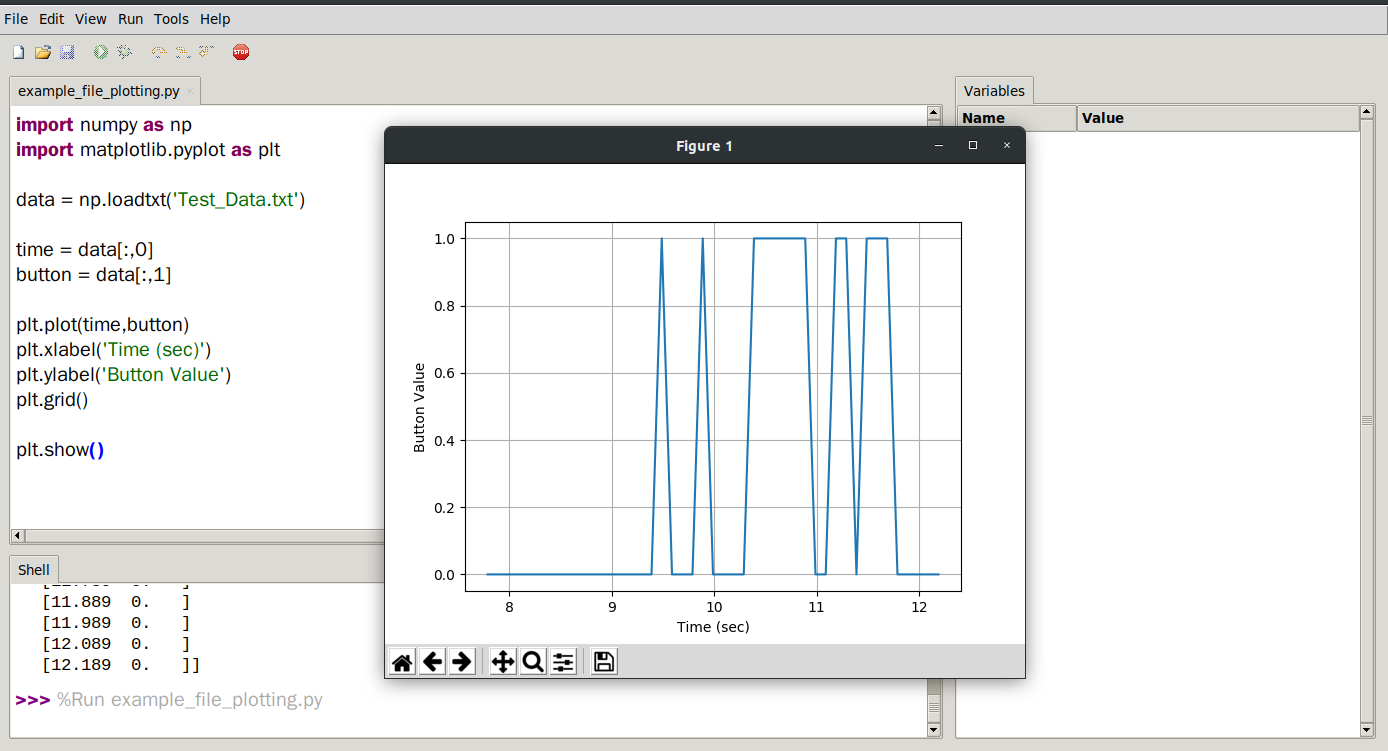
\includegraphics[width=\textwidth]{Figures/plotdata.png}
  \end{center}
\end{figure}
In this example lines 1 and 2 import numpy and matplotlib. Line 4
imports data from the {\it Test\_Data.txt} file and then 6 and 7 save the
first and second columns into time and button. The remaining lines
plot the data and create x and y labels as well as a grid. Hopefully
now you are well versed in taking data and plotting in Python.

\subsection{Assignment}

Upload a PDF with all of the photos and text below included. My
recommendation is for you to create a Word document and insert all the
photos and text into the document. Then export the Word document to a
PDF. For videos I suggest uploading the videos to Google Drive, turn
on link sharing and include a link in your PDF.
\begin{enumerate}[itemsep=-5pt]
\item Use method 1, 2 or 3 and save time and button presses to a text file
\item Include a video explaining which method you are using to record button presses and show yourself pressing the CPX button a few times and recording data. Make sure to wave and introduce yourself - 30\%
\item Copy and Paste your CPX code used to log data - 20\%
\item Copy and paste your Python desktop code used to plot your data - 20\%
\item Include a plot of your button presses with time on the x-axis and button presses on the y-axis (no screenshots) - 30\%
\end{enumerate}


\newpage

\section{Bluetooth on the CircuitPlayground Bluefruit - Method 4}
\label{s:Bluetooth}

\subsection{Parts List}

\begin{enumerate}[itemsep=-5pt]
\item Smart Phone
\item Adafruit BLE Connect App (\href{https://play.google.com/store/apps/details?id=com.adafruit.bluefruit.le.connect}{Play Store}/\href{https://apps.apple.com/us/app/bluefruit-connect/id830125974}{App Store})
\item CircuitPlayground Bluefruit
\item USB Cable
\item Laptop
\end{enumerate}

\subsection{Learning Objectives}
\begin{enumerate}[itemsep=-5pt]
\item Understand the bluetooth module on the CircuitPlayground Bluefruit
\item Learn how to send data via the Bluefruit to your smart phone
\item Understand how to plot data sent via UART
\end{enumerate}

\subsection{Extra Help}

You might find plotting data via bluetooth to be rather difficult and
it was pretty difficult for me until I learned that you can export
data as a txt file rather than a csv file. Before I learned how to do
that I put together
a \href{https://www.youtube.com/playlist?list=PL_D7_GvGz-v0-U3JACRMgldvqQqn2mje9}{4
part series} describing everything in this module. Worst case you can
just watch
the \href{https://www.youtube.com/watch?v=9EHNFdVX9O8&list=PL_D7_GvGz-v0-U3JACRMgldvqQqn2mje9&index=3}{third
video in the series}. The video is 30 minutes but the first 8 minutes
goes through setting up the bluetooth module and the rest of the video
is just on plotting the exported csv data which took me some
time. Note that exporting data as a txt file is the preferred method
as parsing the file is way easier.

{\bf One issue you're going to run into when
you run the codes below is that you won't have some of the modules on
your CPB/CPX.} To fix this you need to download
the \href{https://circuitpython.org/downloads}{CircuitPython
Modules}. You need to click the CircuitPlayground Express or Bluefruit
depending on which one you have and then download the appropriate
version: 6.x, 7.x or 8.x. How do you know what version of CircuitPython
you have? Well head over to your CIRCUITPY drive and open the
boot\_out.txt file and it will tell you the version. Note that this is
the same version as the .UF2 file installed back in the Getting
Started labs (See Chapter \ref{s:Getting_Started}). When you download
the modules it will download a .zip file. Extract the .zip file on
your desktop computer and then open the {\it lib} folder on your
desktop and your CIRCUITPY. You then need to transfer the modules
(ONLY THE ONES YOU NEED) from your desktop to your CPX/CPB. The reason
why you can't copy the entire folder is because the CPB/CPX only has
2MB of flash and the CircuitPython download is 4.1 MB at the time of
this writing. 


\subsection{Getting Started}

I mentioned in the DAQ project that there is technically a
Method4. This is because with bluetooth you can send data from your
phone to your Circuitplayground Bluefruit
(CPB) and you can also send data to your smart phone. Once
the data is on your phone you can export the data to a text file. That
basically means you can use the bluetooth module as another method to
save data from the CPB. There is a lot you can do 
with bluetooth but the bottom line is that  All
code required for this module is on
my \href{https://github.com/cmontalvo251/Microcontrollers/tree/master/Circuit_Playground/CircuitPython/CPB_DataLogger}{Github}. First we're going to run
the \href{https://github.com/cmontalvo251/Microcontrollers/blob/master/Circuit_Playground/CircuitPython/CPB_DataLogger/bluefruit_uart_button.py}{bluetooth\_uart\_button.py}
script which sends button data to your smart phone via something called UART
which is a type of serial communication. It's beyond the scope of this
lesson but serial is digital as opposed to analog which is done using the AnalogIn functions (See Chapter \ref{s:voltage})

\begin{figure}[H]
  \begin{center}
    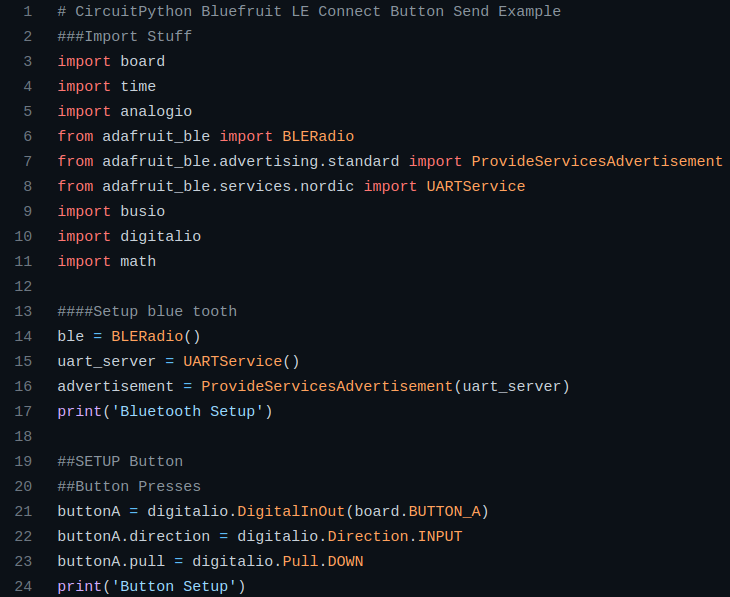
\includegraphics[width=\textwidth]{Figures/bluetooth_code.png}
  \end{center}
\end{figure}
Lines 3-11 import a ton of modules. You'll recognize many of them like
analogio, and time but the new ones are the ones that
say ble. These are the bluetooth modules required for the CPB. Lines
21-24 setup the button so we can log the button via bluetooth and
Lines 14-17 kick of the BLERadio object and the UARTService() to send
data. Line 25 also grabs the current time before the infinite while
loop that way the timer starts closer to zero. 
\begin{figure}[H]
  \begin{center}
    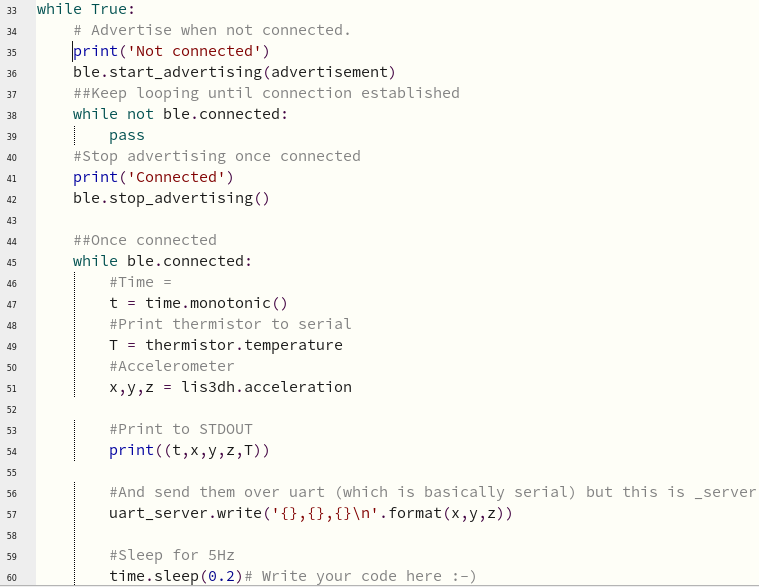
\includegraphics[width=\textwidth]{Figures/bluetooth_code1.png}
  \end{center}
\end{figure}
The code above is the infinite while loop which actually contains 2
while loops. Lines 28-33 prints the name of your bluetooth sensor and
then starts advertising bluetooth to whoever is listening. It will
then enter a while loop from 32-33 until 
bluetooth is connected. Once bluetooth is connected it will enter into
the second while loop from line 39-52. In those lines 40-46 is
responsible for taking all the necessary measurements and printing
them to the serial monitor in Mu. In this case it's only printing the
current time and the value of the button as an integer. {\it
buttonA.value} is either True or False and the {\it int} function
converts that to a 0 or a 1. Line 49 then sends the data
over bluetooth using the UART server. You'll notice in this case the
code is sending t,b by
using the format variable and the 2 empty {} brackets. If you want to
send more data you need to add more empty brackets and more variables
to the format function. When you first save this script your CPB will
not be connected and enter into an infinite while loop where it waits
for your smart phone to connect. If you open your smart phone and open
the Bluefruit Connect App the following screen will pop up. 
\begin{figure}[H]
  \begin{center}
    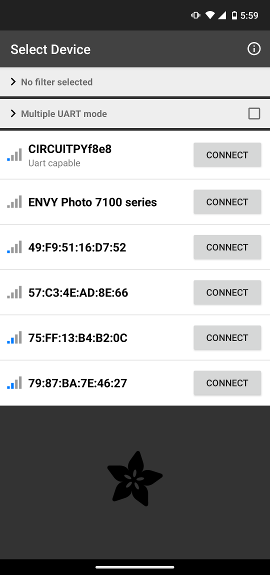
\includegraphics[width=0.3\textwidth]{Figures/phoneapp1.png}
  \end{center}
\end{figure}
In this case there are numerous different bluetooth modules can be
seen but the one you need to click is the one that says
CIRCUITPYf8e8. You will have a different code after CIRCUITPY and you
can figure out what your 4 digit code is by making sure you have the
{\it print('Look for',ble.name)} in your code. Once you do that the
CPB will begin sending time and the button press to your smart phone. 
\begin{figure}[H]
  \begin{center}
    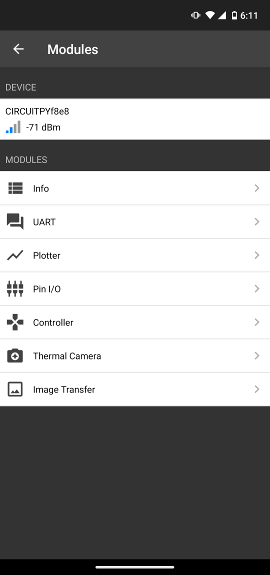
\includegraphics[width=0.3\textwidth]{Figures/phoneapp2.png}
  \end{center}
\end{figure}
There are numerous items you can click. The Controller is very fun for
creating a remote control robot but we're only going to go over the
UART and Plotter tabs. If you click the plotter tab you will be
greeted with a live screen of the data being sent. 
\begin{figure}[H]
  \begin{center}
    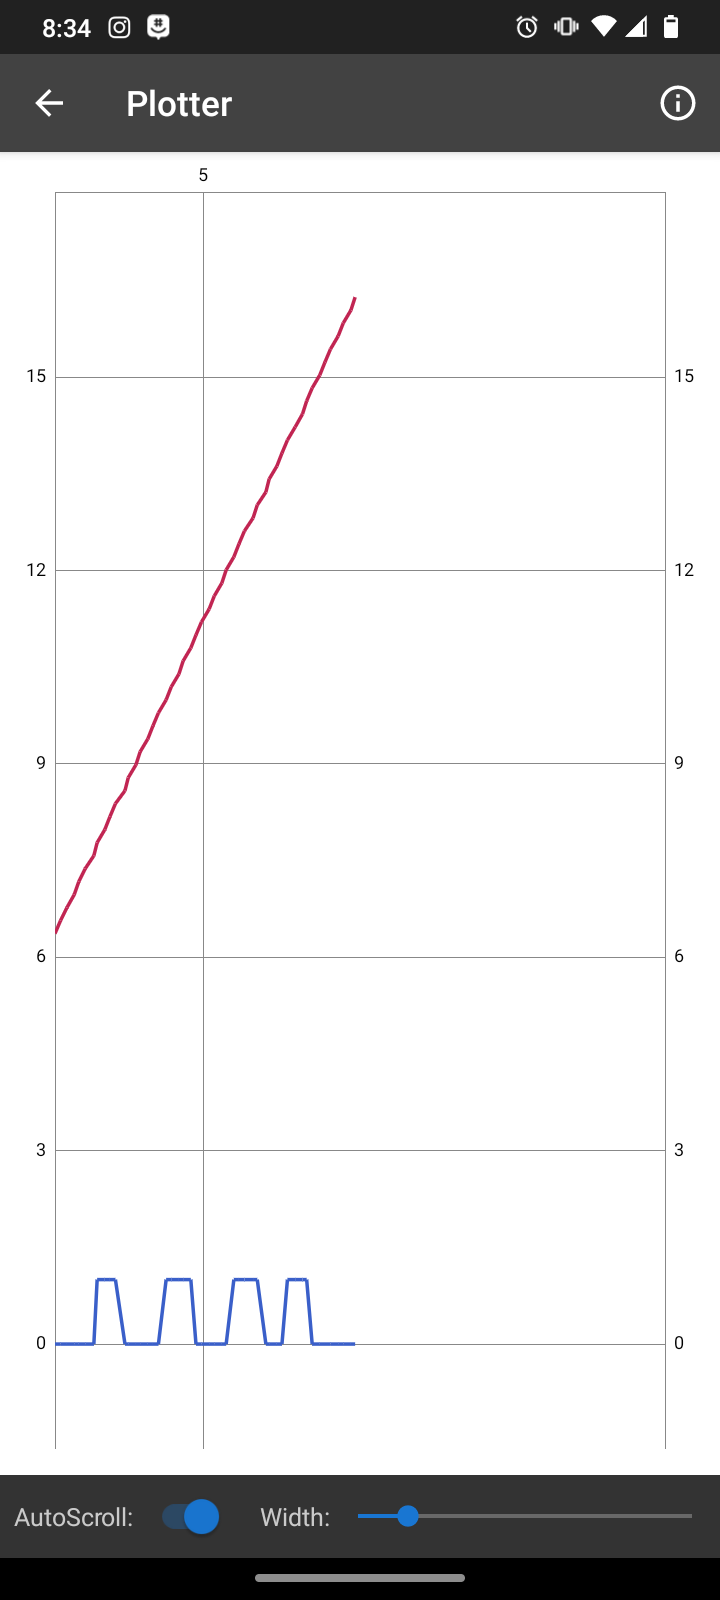
\includegraphics[width=0.3\textwidth]{Figures/phoneapp3.png}
  \end{center}
\end{figure}
In the photo above you can see three data streams that is coming
directly from the CPB. The red line is time and the blue line is the
button value. Notice the blue line goes from 0 to 1 which means I
pressed the button a few times. The red line is always increasing
which kind of messes up the plotter so you can always go back to your
code in Mu and just send your data. This is great for live demonstrations and for
debugging if you need to see data from an experiment and you don't
have access to a laptop with Mu. If you hit the back arrow and then
click UART you will see the raw data come in as text. 
\begin{figure}[H]
  \begin{center}
    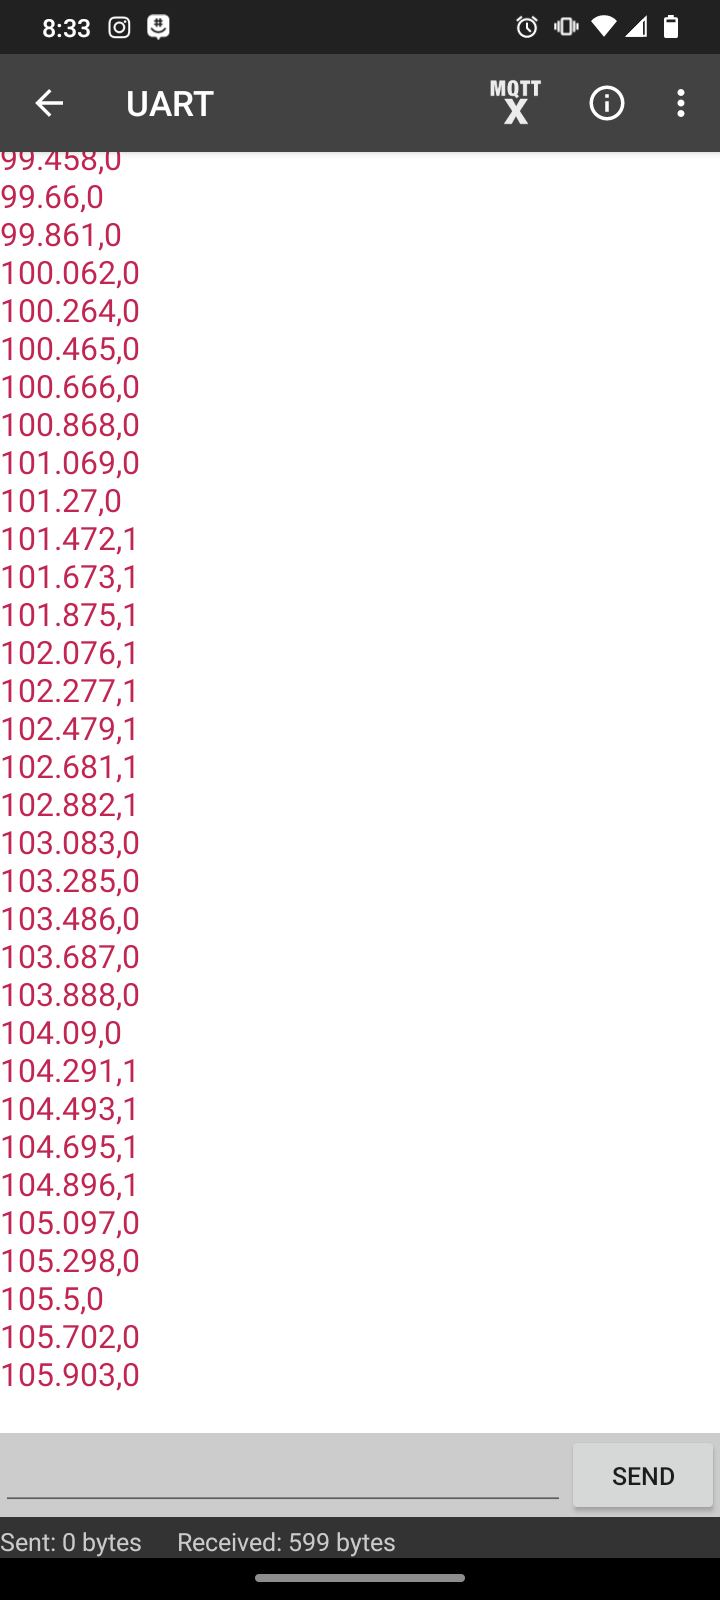
\includegraphics[width=0.3\textwidth]{Figures/phoneapp4.png}
  \end{center}
\end{figure}
Again here you can see the 3 data streams separated by commas. The
very neat thing with the UART tab is that you can click the three
vertical dots in the upper right hand corner and click export to
TXT. The easiest thing for me was to export the data to google drive
and then download the data to my computer. Once I downloaded the TXT file to my
computer and opened it the data file looked like this. 
\begin{figure}[H]
  \begin{center}
    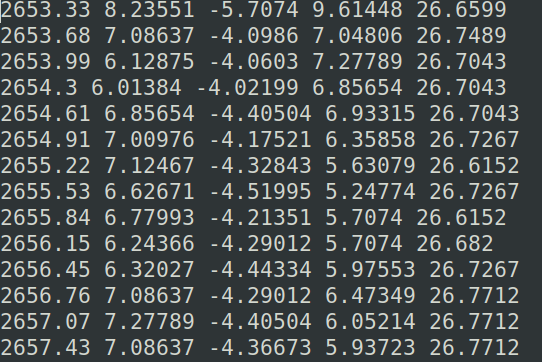
\includegraphics[width=0.8\textwidth]{Figures/csv_fileapp.png}
  \end{center}
\end{figure}
If you export the file as a CSV the data file will look completely
different and it's much more complicated to plot. If you export the
data as a TXT file you just need to use the np.loadtxt command to read
in the data. Note you might have commas in your data file. If there
are commas just use the CTRL+H command and replace all commas with
spaces or use the np.loadtxt('buttonble.txt',delimiter=',')
command. Plotting your button presses should be as simple as the
previous lab thus plotting the button is left as an exercise to the
reader. 

\subsection{Assignment}

This project is similar to the Data Acquisition project only you must use method 4 to save time and button presses to a text file. You must then plot the button presses as a function of time. Remember to add x and y labels to all figures.

Once you've completed the project above, upload a PDF with all of the photos and text
below included. My recommendation is for you to create a Word document
and insert all the photos and text into the document. Then export the
Word document to a PDF. For videos I suggest uploading the videos to
Google Drive, turn on link sharing and include a link in your
PDF. Note that all code must be included in the appendix or you'll be
penalized 10\%. 


\begin{enumerate}[itemsep=-5pt]
\item Include a screenshot from your phone showing the raw UART output - 20\%
\item Include a snippet (5 lines) of your data file - 20\%
\item Include a plot of your button presses with time on the x-axis and button presses on the y-axis (no screenshots) - 40\%
\end{enumerate}


\newpage

\section{Measuring Voltage Across a Potentiometer}
\label{s:voltage}

\subsection{Parts List}

\begin{enumerate}[itemsep=-5pt]
\item Laptop
\item CPX/CPB
\item USB Cable
\item Potentiometer
\item Resistor (the Ohms depends on how large your potentiometer is)
\item Breadboard
\end{enumerate}

\subsection{Learning Objectives}
\begin{enumerate}[itemsep=-5pt]
\item Understand voltage division of resistors in series
\item Measure an analog signal on the CircuitPlayground
\item Understand the binary measurement done by the analog to digital conversion (ADC)
\end{enumerate}

\subsection{Getting Started}

At this point you've learned about analog to digital converters (ADC). It turns out that the CPX has 8 analog ports hooked up to a 3.3V logic 16 bit ADC. The input range on the ADC is 0 to 3.3V and the output range is 0 to 65536 which is $2^{16}$ hence 16 bits. In order to get accustomed to the ADC on the CPX, we’re going to do a simple example where we measure the voltage drop across a potentiometer. You can read about \href{https://www.build-electronic-circuits.com/potentiometer/}{potentiometers online if you wish}. Basically though, a potentiometer is a variable resistance resistor that changes resistance by turning a knob. The knob changes the connection point of a wire and thus the length of the wire. This in turn changes the resistance. Potentiometers come in all shapes and sizes. Here are some \href{https://uk.rs-online.com/web/content/discovery/ideas-and-advice/potentiometers-guide}{potentiometer examples}. I've done this lab with a few potentiometer. Ideally you'd like to have the potentiometer hooked up in series with another resistor so that you end up building a voltage divider but it' possible you can do it without it as shown in the \href{https://learn.adafruit.com/sensor-plotting-with-mu-and-circuitpython/potentiometer}{figure below} (Courtesy of \href{https://learn.adafruit.com/u/kattni}{Kattni Rembor}).
\begin{figure}[H]
  \begin{center}
    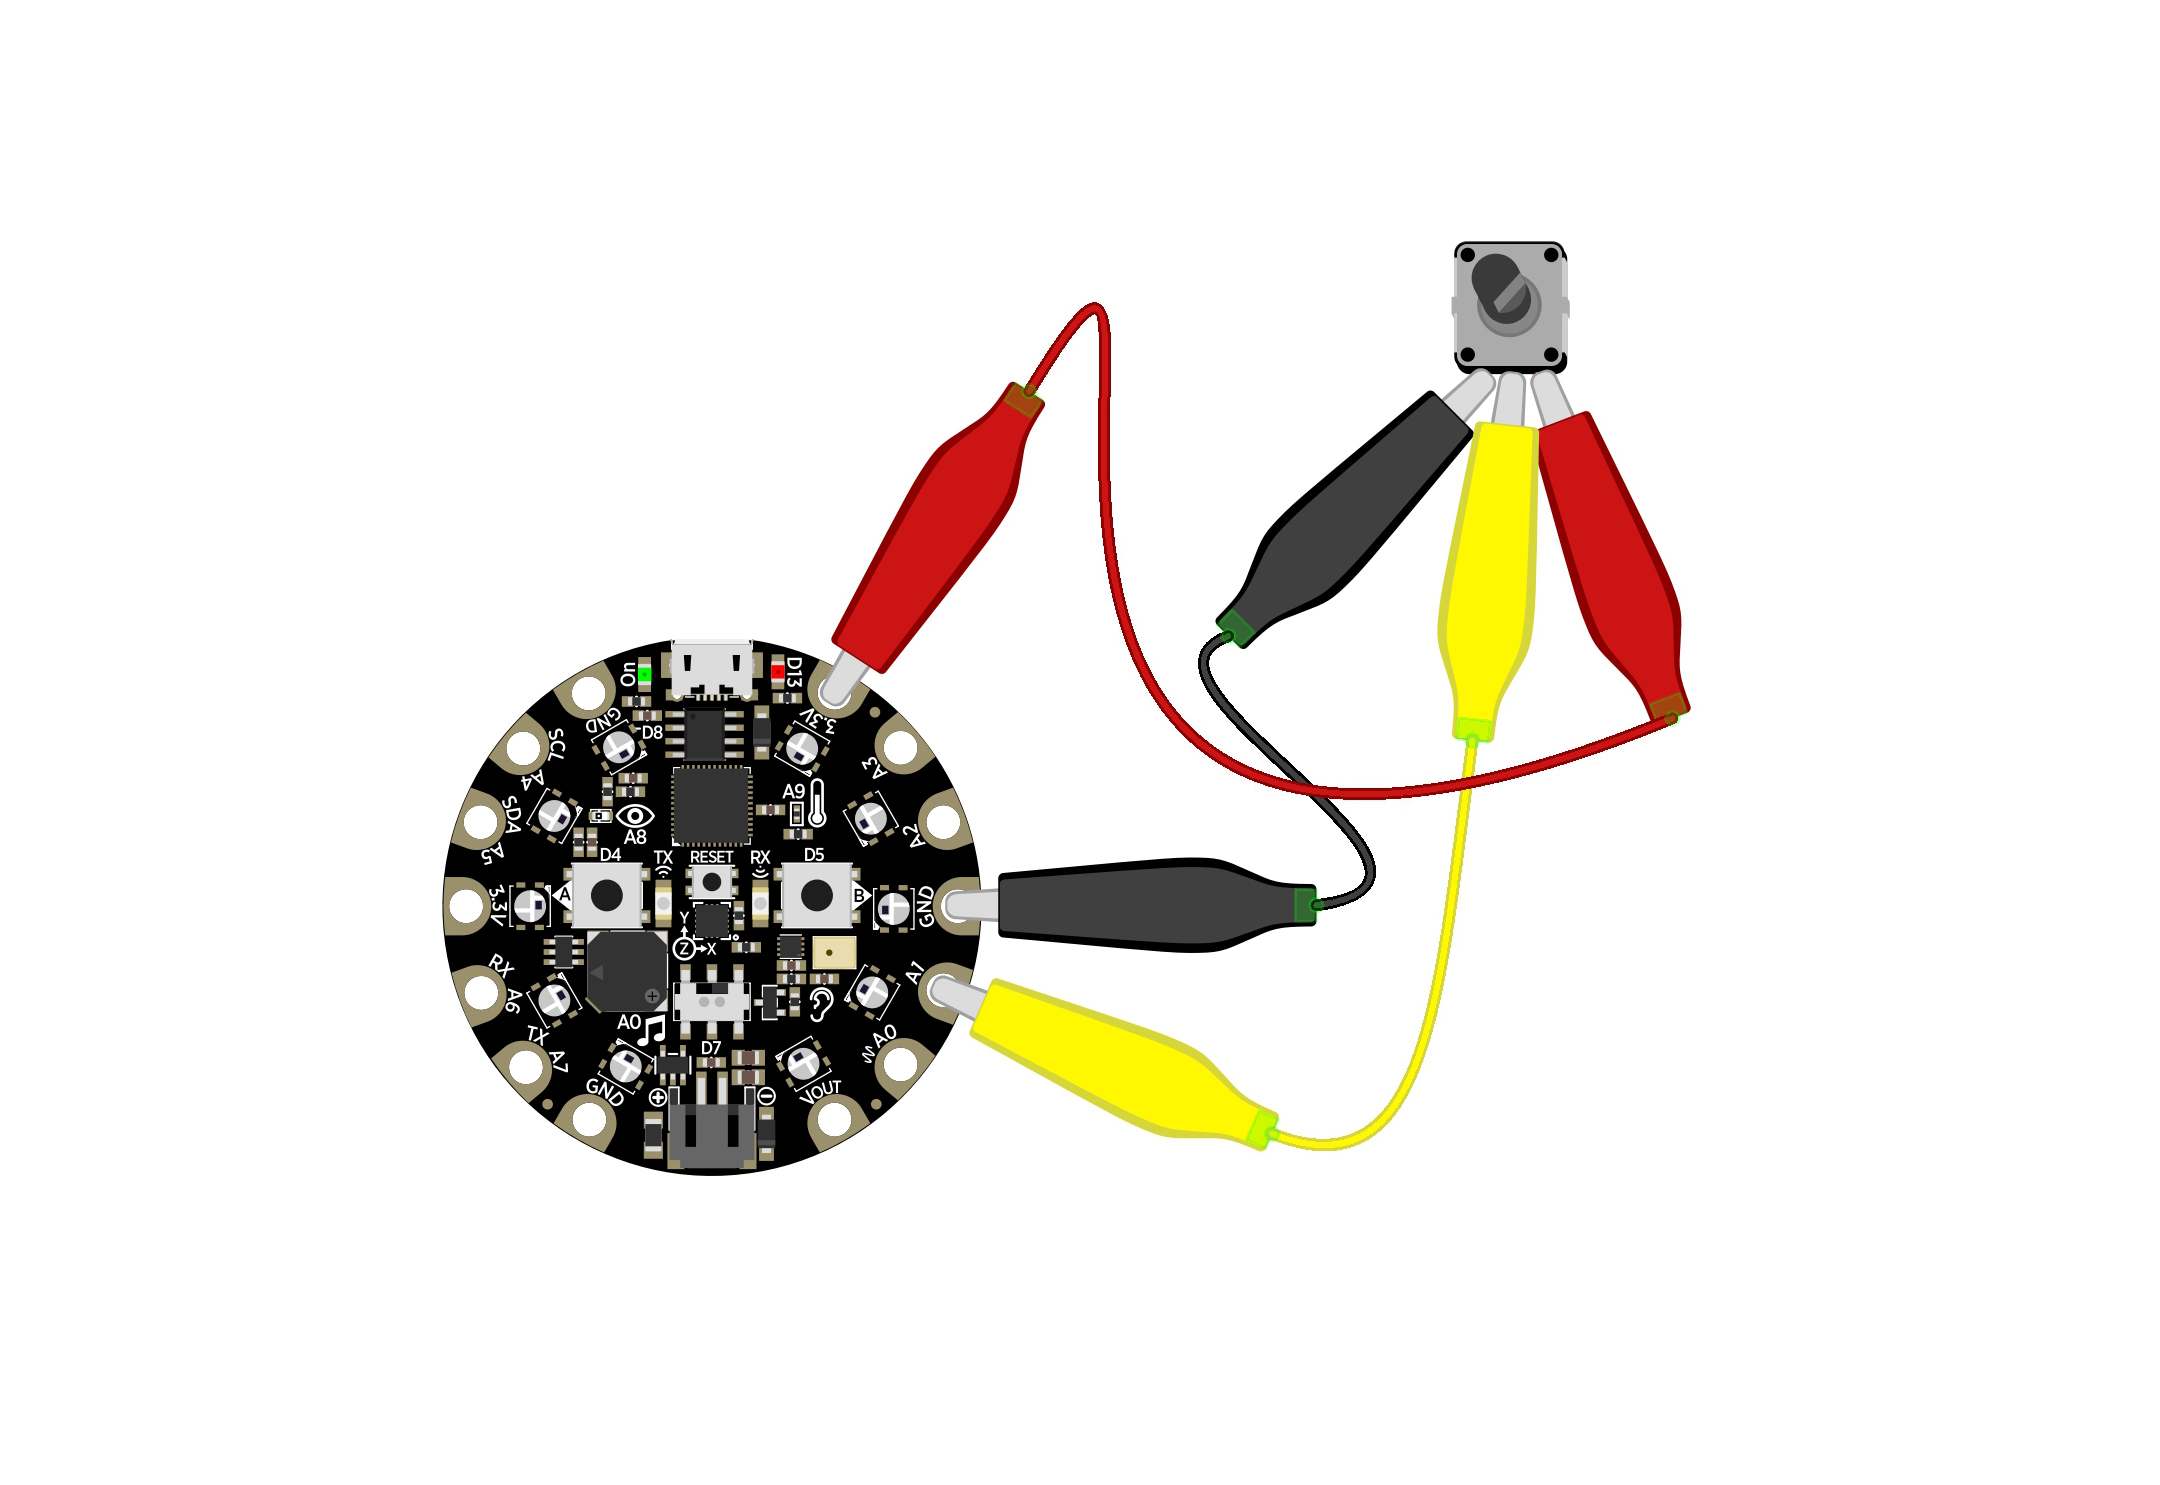
\includegraphics[width=0.8\textwidth]{Figures/sensors_PlottingMuPotentiometer_bb.jpg}
  \end{center}
\end{figure}
Here’s my circuit all hooked up without a resistor in series. Two legs are connected to 3.3V and GND while the middle leg of the potentiometer is connected to pin A2.
\begin{figure}[H]
  \begin{center}
    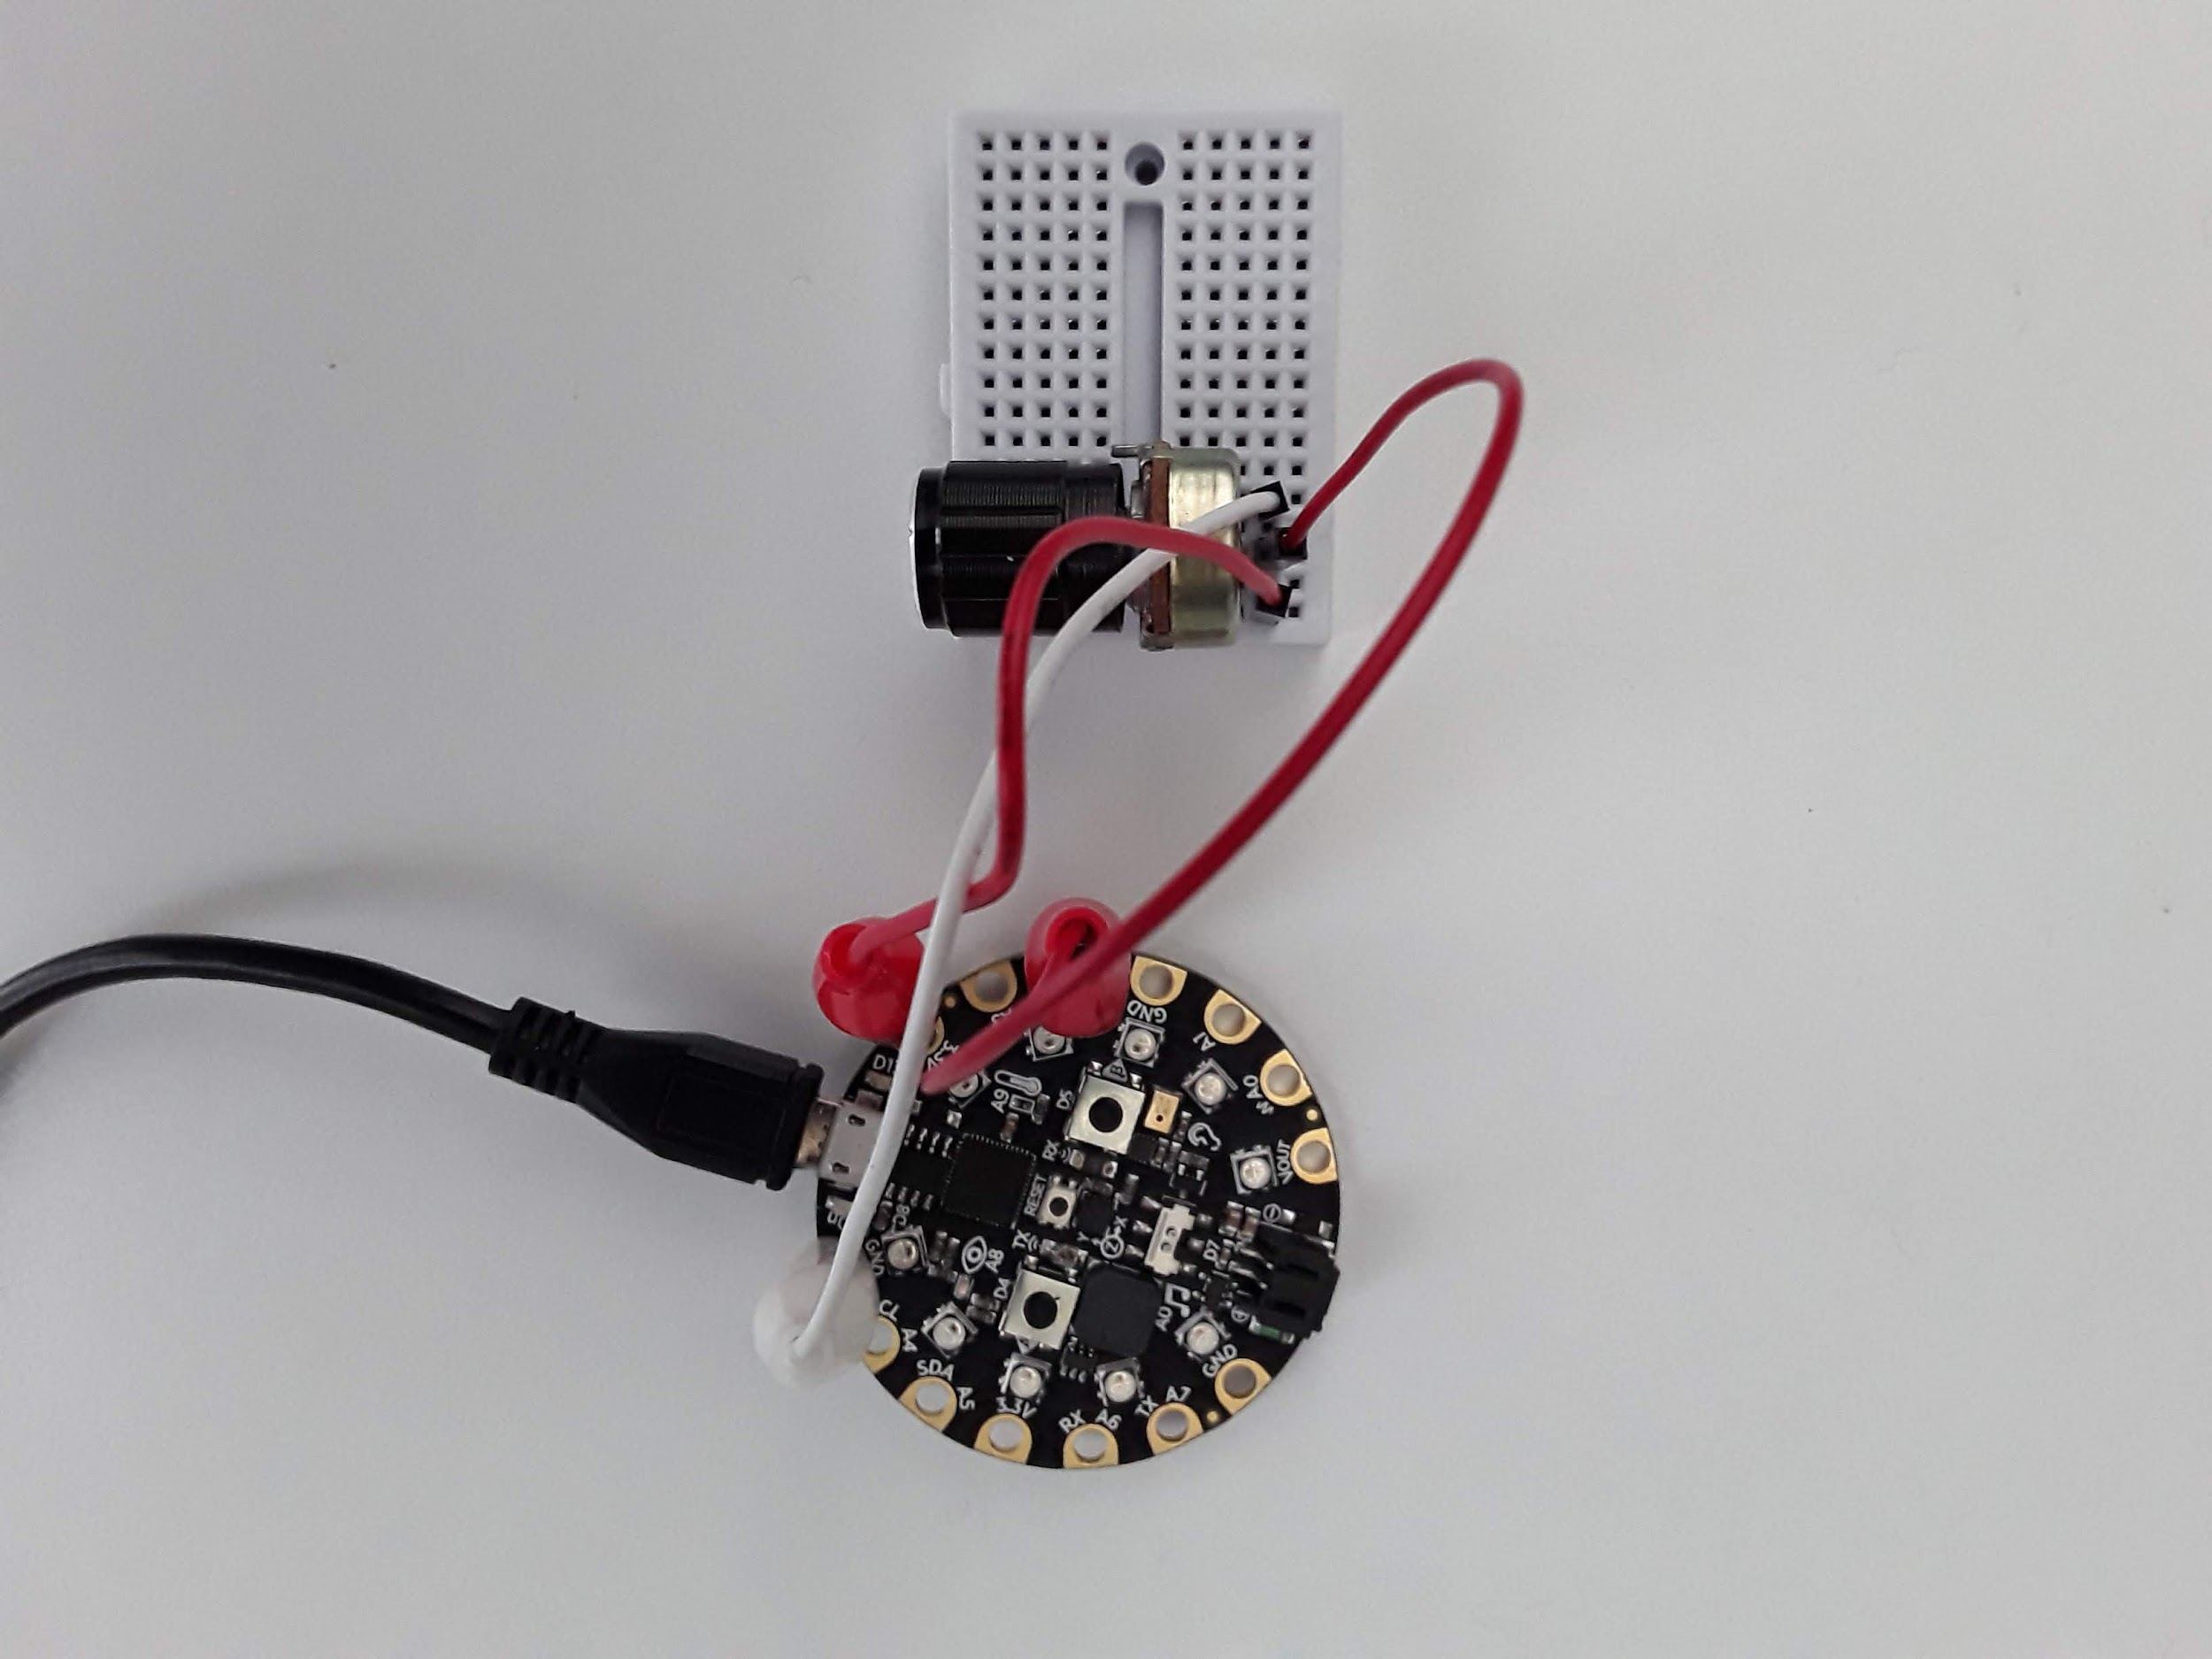
\includegraphics[width=0.8\textwidth]{Figures/potentiometer1.jpeg}
  \end{center}
\end{figure}
{\bf As I said before, some potentiometers do not have enough resistance when turned all the way down. I suggest that you put a resistor in between the third leg and ground. Some experimenters have melted plastic or gotten really hot. One student even blew up a potentiometer.} Here is my circuit with a resistor in series.
\begin{figure}[H]
  \begin{center}
    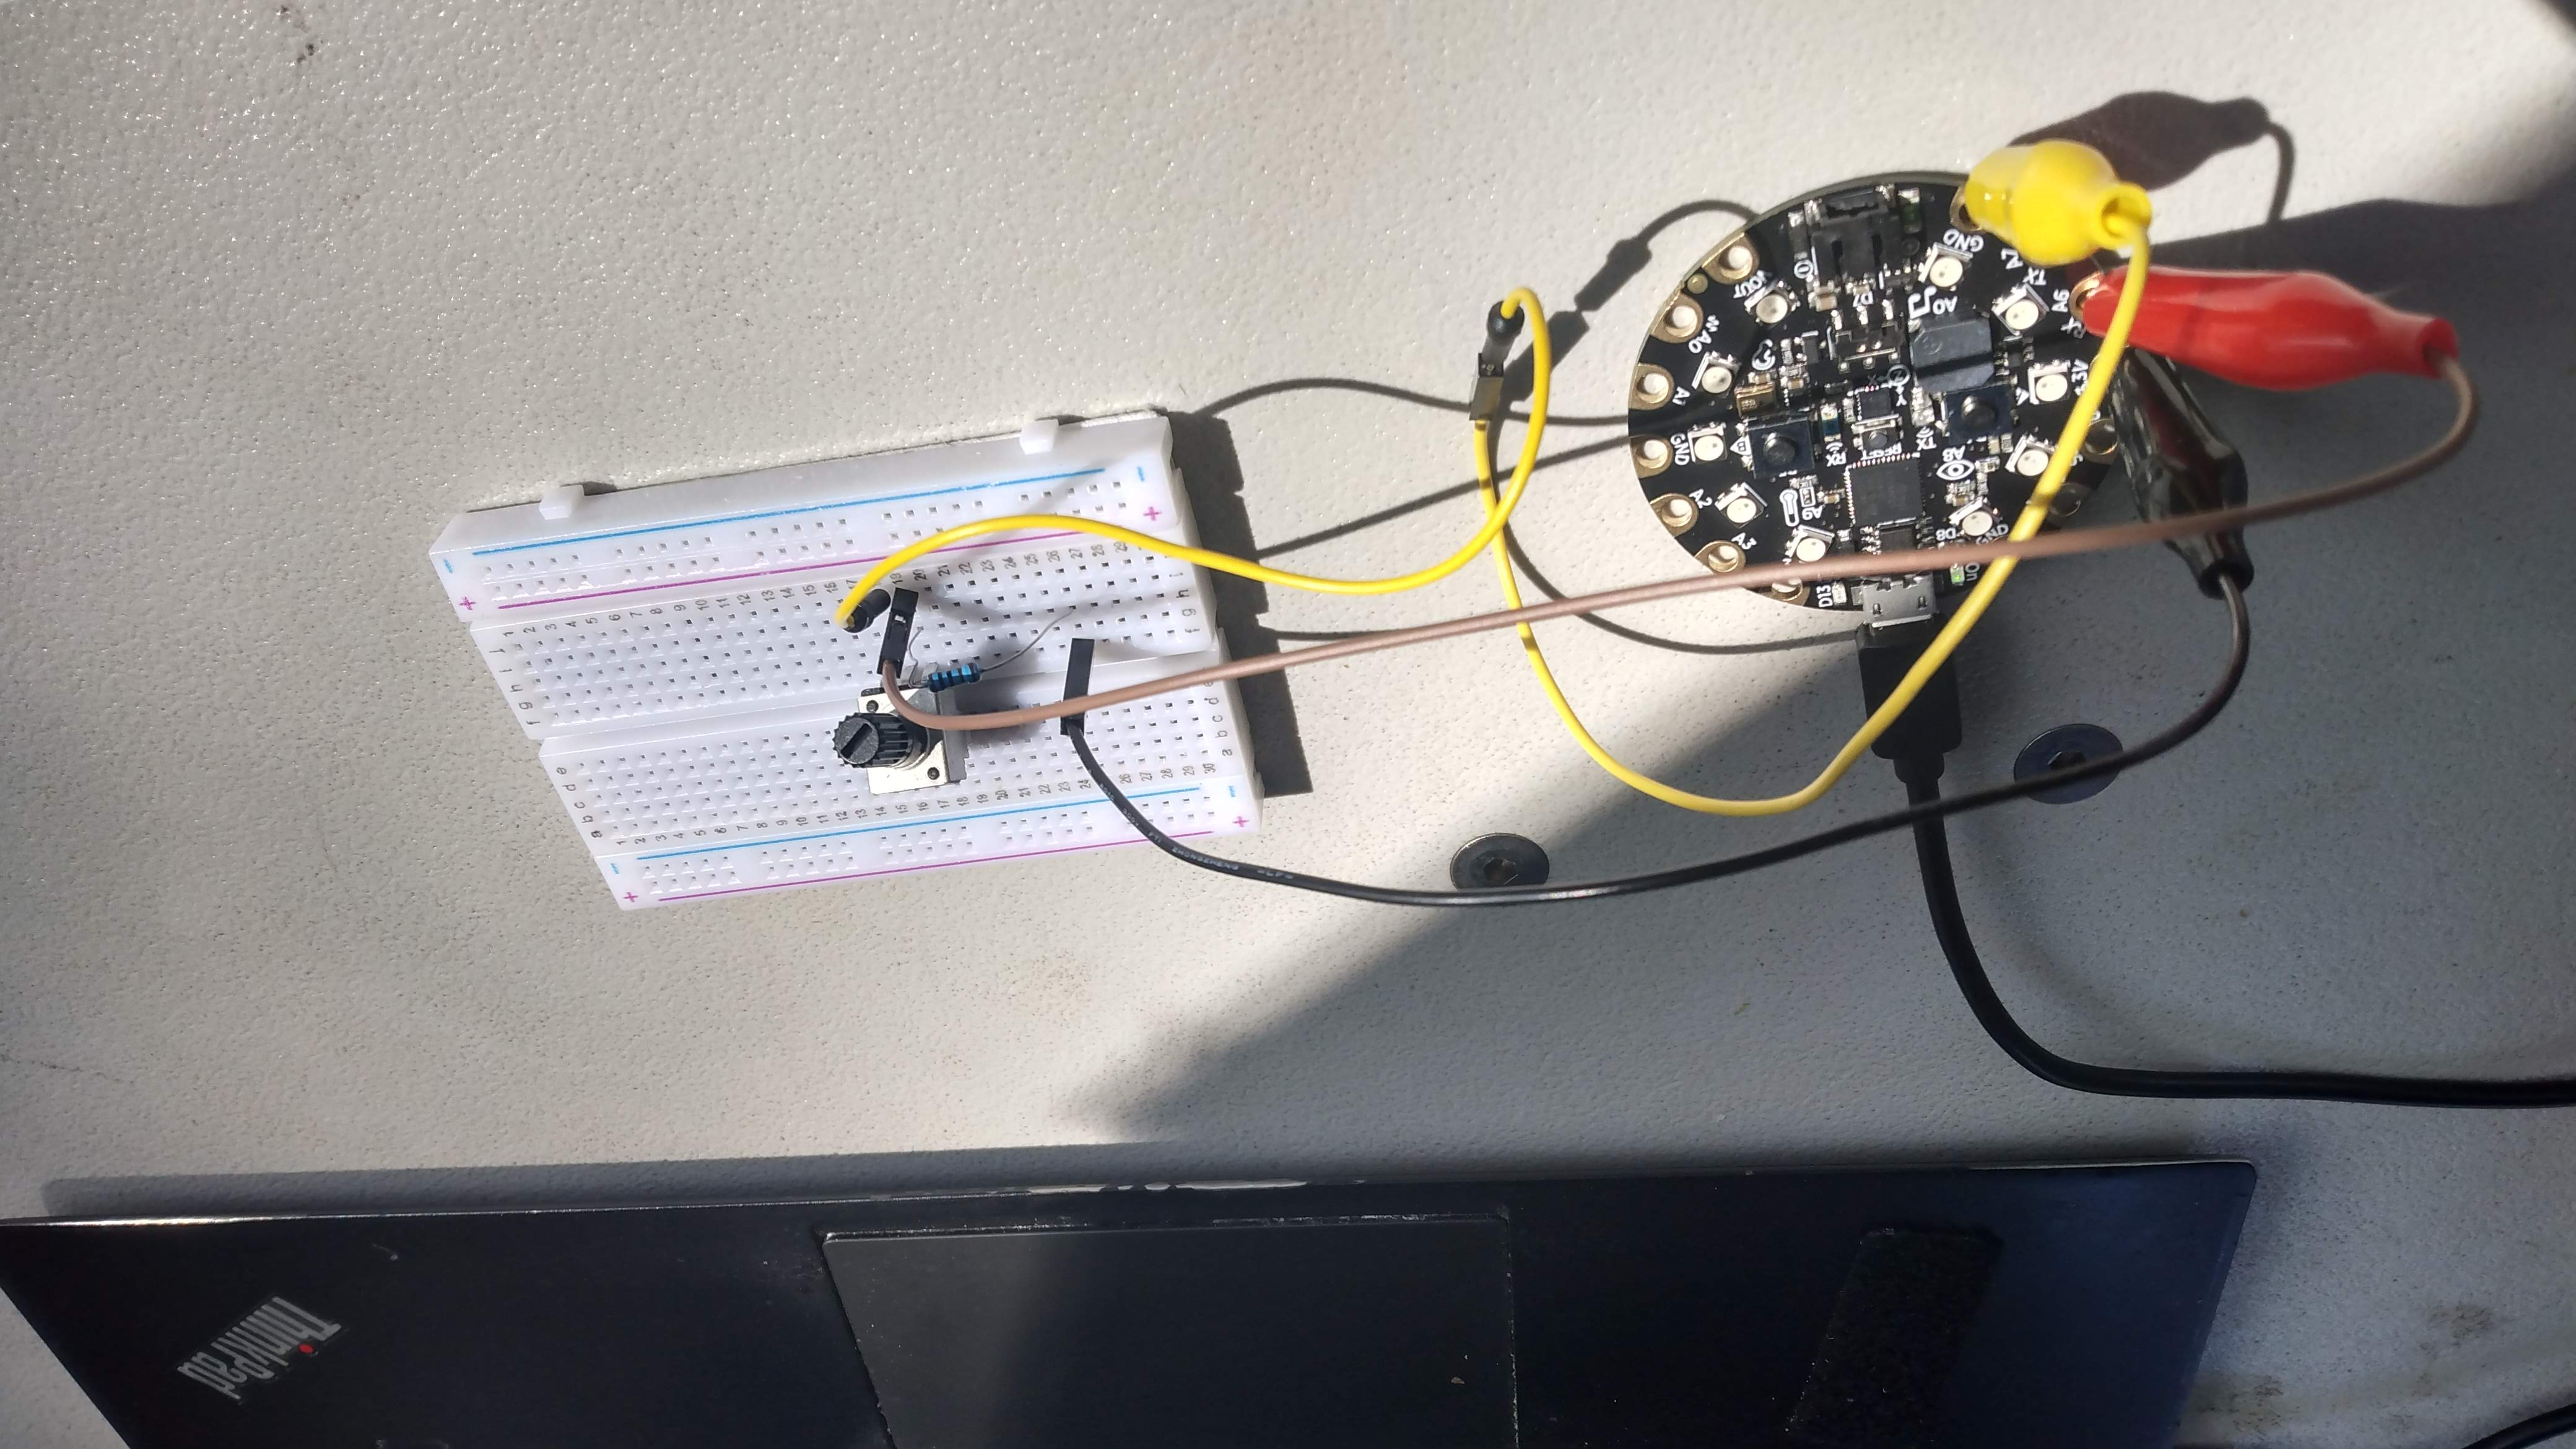
\includegraphics[angle=180,width=0.8\textwidth]{Figures/Potentiometer_Alternate.jpg}
  \end{center}
\end{figure}
There is a relevant \href{https://learn.adafruit.com/adafruit-circuit-playground-express/circuitpython-analog-in}{Adafruit Learn Tutorial} to help with the {\it analogio} module but I’ll explain the minimum required here to get some analog values plotted in {\it Plotter} and Python on your computer. First let’s take a look at some \href{https://github.com/cmontalvo251/Microcontrollers/blob/master/Circuit_Playground/CircuitPython/Analog/analog_simple.py}{simple example code} to read an analog signal and plot it using the {\it Plotter}.
\begin{figure}[H]
  \begin{center}
    \includegraphics[width=0.5\textwidth]{Figures/analogio.png}
  \end{center}
\end{figure}
In the example code above, lines 1-3 again import the necessary modules with {\it analogio} being the new module here. Line 5 creates the analog object by attaching pin A2 to the analog function. Lines 7-9 then simple read the analog value and print it to {\it Serial} and the {\it Plotter}. Running this code on my laptop and turning the knob on the potentiometer produces this output. My potentiometer has a very large knob on the front and is easy to turn. Some potentiometers have a small screw on top that you need to turn with a screwdriver. Turning the screw or the knob results in chaning the resistance and therefore changing the voltage read by the CPX.
\begin{figure}[H]
  \begin{center}
    \includegraphics[width=\textwidth]{Figures/analogio_mu.png}
  \end{center}
\end{figure}
For this lab I want you to spin the potentiometer all the way to one side and then the other while recording time and the analog value. I then want you to plot the data with time on the x-axis and voltage on the y-axis. Remember to convert a digital output to voltage you just need to use the equation below where D is the raw value from the analog port. 3.3V is the range of the ADC and $2^{16}$ is the maximum value the ADC can represent.
\begin{equation}
V = \frac{3.3D}{2^{16}}
\end{equation}
After doing this experiment myself, this is the plot I obtain. The code is not provided as reading data and plotting has been discussed in a previous lab (See chapter \ref{s:daq}). From the screenshot though you can see how I convert the digital output to an analog signal.
\ \\
\ \\
{\bf NOTE THAT ON LINE 6 IT READS}
\begin{verbatim}
time -= time[0]
\end{verbatim}
{\bf Notice the minus sign in front of the equal sign. That effects a lot.}
\begin{figure}[H]
  \begin{center}
    \includegraphics[width=\textwidth]{Figures/plotting_analogio.png}
  \end{center}
\end{figure}
Your assignment for this lab is to do the same as I’ve done above. Wire up the potentiometer, read the analog signal and plot it in Python on your desktop computer. I’ve made some youtube videos on first just \href{https://youtu.be/_gnDvPOvPqk}{creating the circuit and plotting the data} and then another video where I \href{https://youtu.be/9UF3OVUIYjU}{write data to the CPX using method 3}.

\subsection{Assignment}

For this assignment you are to wire up a potentiometer and read the voltage across the potentiometer using the analog to digital converter on the CPX. You are to record both time and voltage as you rotate the potentiometer and then plot that as a function of time. Specific requirements are shown below.

Once you've completed the project above, upload a PDF with all of the photos and text
below included. My recommendation is for you to create a Word document
and insert all the photos and text into the document. Then export the
Word document to a PDF. For videos I suggest uploading the videos to
Google Drive, turn on link sharing and include a link in your
PDF. Note that all code must be included in the appendix or you'll be
penalized 10\%. 


\begin{enumerate}[itemsep=-5pt]
\item Include a photo of your circuit showing the potentiometer wired up to an analog pin on your CPX/CPB - 20\%
\item Include a screenshot of Mu with the Plotter open showing the value of the potentiometer. The code in Mu also needs to also show the same analog pin as your potentiometer. - 20\%
\item Plot your digital output (raw potentiometer analog value) vs time - 20\%
\item Then convert your digital output (Do) to voltage and plot that vs time - 20\% 
\end{enumerate}


\newpage

\section{Wind Speed from Pitot Probe}

\subsection{Parts List}

\begin{enumerate}[itemsep=-5pt]
\item Laptop
\item CPX/CPB
\item USB Cable
\item Alligator Clips (x3)
\item Pitot Probe (Not included in kit at the moment so will need to buy this separately or borrow one)
\item Breadboard
\end{enumerate}

\subsection{Learning Objectives}
\begin{enumerate}[itemsep=-5pt]
\item Understand how pitot probes works
\item Understand the relationship between a voltage signal from a pitot probe to a pressure value
\item Understand the relationship between pressure and windspeed
\end{enumerate}

\subsection{Getting Started}

Although a CPX has numerous sensors built in, you can easily augment the capabilities of the CPX using either I2C or just the ADC on board the CPX. In this lab, if you purchased a \href{https://www.amazon.com/Hobbypower-Airspeed-MPXV7002DP-Differential-controller/dp/B00WSFWO36/ref=sr_1_3?dchild=1&keywords=Airspeed+sensor+kit&qid=1590532161&sr=8-3}{pitot probe} you will be able to do this assignment. Since you don’t need the pitot probe for very long you can always borrow one from some other team. Let’s talk about the hardware and the wiring to get this to work.
\begin{figure}[H]
  \begin{center}
    \includegraphics[width=\textwidth]{Figures/pitot_probe_circuit.jpeg}
  \end{center}
\end{figure}
The pitot probe has two pressure taps that measure ambient pressure and stagnation pressure. These taps move through two silicon tubes to a pressure transducer that has a strain gauge in separating both pressures. When the pressure on one side of the transducer is larger than the other, it will flex the membrane and create strain. This strain runs through a wheatstone bridge with a voltage offset to the pin labeled analog. The transducer has 3 pins, +5V, GND and Analog. It is pretty straightforward how to wire this up but remember that +5V needs to go to VOUT, GND to GND and Analog to any analog pin. I chose pin A2. At that point it’s very simple to just print the analog signal in bits to Serial. I’ve done this below. The code is the same \href{https://github.com/cmontalvo251/Microcontrollers/blob/master/Circuit_Playground/CircuitPython/Analog/analog_simple.py}{analog code} that we’ve used in the past.
\begin{figure}[H]
  \begin{center}
    \includegraphics[width=0.5\textwidth]{Figures/analogio.png}
  \end{center}
\end{figure}
The goal of the experiment is to take pitot probe data for 15 seconds with no wind, then 15 seconds of data with a fan on and then 15 seconds of no wind data. You’ll need to use one of the datalogging methods (See chapter \ref{s:daq}) to log both time and pitot probe analog value. Once you have that data, import the data into Python on your desktop computer and convert the signal to windspeed. In order to convert the analog value to windspeed you need to first convert the analog value to voltage. Remember that the ADC on the CPX is going to convert the analog signal from the pitot probe to a digital output. So use this equation first to convert the analog signal (which I call D) to voltage. The 2 to the 16th power represents the 16 bit ADC.
\begin{equation}
V = \frac{3.3D}{2^{16}}
\end{equation}
Before converting Voltage to windspeed we need to first subtract off the bias from the pitot probe. I explain this process in this \href{https://www.youtube.com/watch?v=e4xs9Ky7_YI&feature=youtu.be}{accelerometer video}. I’ve done this project before and have posted a video on Youtube about \href{https://youtu.be/jSLIRC1cfvE}{Converting Pitot Probe Data to Windspeed}. {\bf \it There is a typo in the video. V1 is supposed to have a sqrt())}. Once you have computed the bias you can compute the change in pressure using the equation below which converts the change in voltage to Pascals ($V_b$ is the voltage bias you obtain when the wind is off). The data sheet states that the voltage is linearly proportional to pressure in Pascals which is nice.
\begin{equation}
P = 1000(V-V_b)
\end{equation}
Using pressure, the equation below can be used to compute windspeed, where U is the windspeed and the density at sea-level ($\rho$) is 1.225 $kg/m^3$.
\begin{equation}
U = \sqrt{\frac{2P}{\rho}}
\end{equation}
Using your data, create a plot of windspeed with time on the x-axis and windspeed on the y-axis. Some steps that might help you as you complete this project. First, have Mu plot the voltage coming from the pitot probe. If you’ve done everything right it will not be zero. The data sheet says there’s an offset voltage of 2.5V so you will hopefully get something around 50,000 when you don’t blow into the pitot probe. 50,000 multiplied by 3.3/$2^16$ is around 2.5V. Make a note of that average value you get so you can subtract it off later. Once you’ve verified you’re reading the pitot probe correctly, blow into the pitot probe and using the Plotter or Serial, verify that the analog signal increases. If the signal decreases, it means the pressure taps on the pressure transducer are backwards and you need to flip them. Either that or just flip the sign in your plotting routine on your computer but flipping the tubes might be easier for you. Hopefully when you do this lab you will get some data that looks like this. In this Figure you’ll see that when the fan wasn’t running the signal was something around 49,800 which is fine. It means your bias is around 2.5 volts. Every pitot probe and circuit will be different. You can then convert this signal to voltage then and then pressure and then finally wind speed.
\begin{figure}[H]
  \begin{center}
    \includegraphics[width=\textwidth]{Figures/pitot_probe_data.png}
  \end{center}
\end{figure}
The code to accomplish this is relatively simple and a portion of the code is shown below. You’ll see that when I subtracted the bias from the voltage I also zeroed out any negative values. That is, any delta voltage less than zero was set to zero. A couple of things about this chart. The data from the pitot probe is super noisy which means attaching a \href{https://youtu.be/zTGa4sk6UZE}{complementary filter} is probably a good idea provided you don’t over filter the signal and run into \href{https://youtu.be/8F_8st_8MmA}{aliasing issues}. You can see that I implemented an offline complementary filter and plotted it in the orange line which helps the noise issue quite a bit. You’ll also notice that the noise is about 2 m/s. It turns out that pitot probes are actually not very accurate lower than about 2 m/s. They would be great for an airplane or you driving down the highway but they wouldn’t be very good to take wind data outside on a calm day.
\begin{figure}[H]
  \begin{center}
    \includegraphics[width=\textwidth]{Figures/pitot_probe_final.png}
  \end{center}
\end{figure}

\subsection{Assignment}

Once you've completed the project above, upload a PDF with all of the photos and text
below included. My recommendation is for you to create a Word document
and insert all the photos and text into the document. Then export the
Word document to a PDF. For videos I suggest uploading the videos to
Google Drive, turn on link sharing and include a link in your
PDF. Note that all code must be included in the appendix or you'll be
penalized 10\%. 


\begin{enumerate}[itemsep=-5pt]
\item If you borrowed a pitot probe return the pitot probe - Pass/Fail - If you don’t return the pitot probe you receive a zero
\item Include a video of you taking data and explaining the circuit (make sure you are in the video) - 50\%
\item Include a plot of the raw analog signal vs time just like I did above - 20\%
\item Include a plot of windspeed vs time as I did above - 20\%
\item Filter your signal using an offline complementary filter and include it in your plot like I did above - 10\%
\end{enumerate}


\newpage

\section{Circuit Playground (CPX/CPB) Modules}
\label{s:Modules}

\subsection{Parts List}

\begin{enumerate}[itemsep=-5pt]
\item Laptop
\item CPX/CPB
\item USB Cable
\end{enumerate}

\subsection{Learning Objectives}
\begin{enumerate}[itemsep=-5pt]
\item Understand the different sensors on the Circuitplayground
\item Learn the difference between high level and low level control
\item Get more practice plotting data from onboard sensors
\end{enumerate}

\subsection{Extra Help}
If you need extra help on this assignment I have uploaded a youtube
video where I \href{https://www.youtube.com/watch?v=ceI0uw3ICE0}{read
the temperature and accelerometer from the CircuitPlayground
Bluefruit} 

\subsection{Getting Started}

The CPX has numerous built-in sensors. These include a light sensor,
an IR sensor, an accelerometer, a microphone, a speaker, some
neopixels, a temperature sensor and 8 analog inputs with ADCs and even
I2C (pronounced I squared C - it’s a kind of serial communication)
that you can use to easily hook up more sensors to it. We're not going
to utilize all of these sensors since that would be a rather large
project. Instead we’re going to learn how to use the temperature,
light and sound sensors as well as the accelerometer. For each of
these examples there is a relatively easy way to access the sensors
using a built-in module called {\it
adafruit\_circuitplayground.express} if you are using the CPX. If you
are using the CPB you need to type {\it
adafruit\_circuitplayground.bluefruit}. It’s a very nice module
because it imports everything on the board. The problem is you can run
into module conflicts. This happens when two different modules try to
access the same pins on the CP. Sometimes if you import {\it
adafruit\_circuitplayground} you won’t be able to import some other
modules. {\bf Note you might need to add the {\it
adafruit\_circuitplayground} library to your lib/ folder on your
CIRCUITPY drive}. Due to this module conflict issue, there are some
low level control commands you can use to access each of the sensors
on board. We're obviously going to learn the low level control method
first and then I’ll show you how to access the sensors using the {\it
adafruit\_circuitplayground} module. {\bf If you get a “currently in
use” error it means you have a module conflict. Hence why I’m showing
you the low level control method}. {\bf One issue you're going to run into when
you run the codes below is that you won't have some of the modules on
your CPB/CPX.} To fix this you need to download
the \href{https://circuitpython.org/downloads}{CircuitPython
Modules}. You need to click the CircuitPlayground Express or Bluefruit
depending on which one you have and then download the appropriate
version: 6.x, 7.x or 8.x. How do you know what version of CircuitPython
you have? Well head over to your CIRCUITPY drive and open the
boot\_out.txt file and it will tell you the version. Note that this is
the same version as the .UF2 file installed back in the Getting
Started labs (See Chapter \ref{s:Getting_Started}). When you download
the modules it will download a .zip file. Extract the .zip file on
your desktop computer and then open the {\it lib} folder on your
desktop and your CIRCUITPY. You then need to transfer the modules
(ONLY THE ONES YOU NEED) from your desktop to your CPX/CPB. The reason
why you can't copy the entire folder is because the CPB/CPX only has
2MB of flash and the CircuitPython download is 4.1 MB at the time of
this writing. 


\subsection{Low Level Control}

\subsubsection{Light}

The light sensor on the CPX is just a simple photocell wired in series
with a resistor. There is a lab on photocells (See
chapter \ref{s:photocell} if you'd like to do that lab first to learn
about photocells. The GND leg of the photocell is connected to pin
A8. You can check the pin by looking at the graphic of an eye on the
CPX and taking a look at the digital pin next to it. We’ve already
learned how to {access analog pins (See chapter \ref{s:voltage}) in a
previous lab so just use
the \href{https://github.com/cmontalvo251/Microcontrollers/blob/master/Circuit_Playground/CircuitPython/Analog/analog_simple.py}{code
from that lab} and change the pin to A8. Here’s what my code looks
like when I change the pin to A8. I also brought the Plotter up and
moved my finger in front of the light to make sure the light was
working. Verify that your CPX responds the same way before moving on. 
\begin{figure}[H]
  \begin{center}
    \includegraphics[width=\textwidth]{Figures/modules_light_mu.png}
  \end{center}
\end{figure}
\subsubsection{Sound}
The sound sensor uses the audiobusio library and creates a mic object
using the (Pulse Density Modulation) PDM library. You have to set the
sample rate and the number of bits to use to capture the data. We’re
going to set the bits to 16 to utilize the whole spectrum and then set
the sample rate to 16 kHz. It’s not quite 44.1 kHz like most modern
microphones but it will do. After creating the mic object we have to
compute some root mean squared values and thus two functions are
defined before the while true loop in the code. The code itself is
shown below. The code starts on line 22 because the
first \href{https://learn.adafruit.com/adafruit-pdm-microphone-breakout/circuitpython}{22
lines are copyright from Dan Halbert, Kattni Rembor, and Tony DiCola
from Adafruit Industries}. I have edited the code a bit to fit my
needs and
uploaded \href{https://github.com/cmontalvo251/Microcontrollers/blob/master/Circuit_Playground/CircuitPython/Audio/record_sound_simple.py}{my
version to Github}. In the code line 23-27 import standard modules as
well as some new ones. The array module is used to create array like
matrices. The math module is used to compute functions like cos, sin,
and sqrt. Then of course the audiobusio module is used to create the
mic object on line 42. Notice the two functions defined on 33 and 39
which create a function for computing the mean and for computing the
normalized root mean square value of the data stream. Basically what’s
going to happen is we’re going to record 160 samples as defined on
line 160. So on line 43 we create a hexadecimal array (hexademical:
base 16 hence the num\_bits set to 16 on line 31) with 160 zeros. In
the while true loop we’re going to sleep for 0.01 seconds and then
record some samples. Since we’re sampling at 16 kHz the time it takes
to record 160 samples is 160/16000 = 16/1600 = 1/100 = 0.01
seconds. Since we’re taking 160 samples we need to compute some sort
of average which is why the normalized root mean square value is
computed on line 48. 
\begin{figure}[H]
  \begin{center}
    \includegraphics[width=\textwidth]{Figures/sound_code.png}
  \end{center}
\end{figure}
When I run this code and talk normally into the microphone. I get this
output in the Plotter. You’ll notice that the data is pretty noisy in
the beginning. It’s possible we could increase the number of samples
we take each loop by editing line 30 but that would slow down our
code. So there’s a tradeoff between filtering here and speed. That’s
something will investigate in some later labs. 
\begin{figure}[H]
  \begin{center}
    \includegraphics[width=\textwidth]{Figures/sound_mu.png}
  \end{center}
\end{figure}
\subsubsection{Temperature}
The temperature sensor is actually
a \href{https://en.wikipedia.org/wiki/Thermistor}{thermistor}. A
thermistor is basically a thermometer resistor which means the
resistance depends on temperature. This means that you can read the
analog signal coming from the thermistor just by reading the analog
signal from pin A9. If you look for the thermometer symbol on the CPX
you’ll see pin A9. Therefore, it is possible to just use the analogio
library and just read in the analog voltage but in order to convert to
celsius and then fahrenheit you need to use some heat transfer
equations to convert the analog signal to celsius. Thankfully the
folks at Adafruit have done it again with an {\it
adafruit\_thermistor} module. If you head over to
their \href{https://github.com/adafruit/Adafruit_CircuitPython_Thermistor/blob/master/adafruit_thermistor.py}{github
on this module} you’ll see the relevant conversion under the
definition temperature which at the time of this writing is on line
86. \href{https://learn.adafruit.com/thermistor/circuitpython}{The
Adafruit Learn system also does a bit of work to explain the
conversion from voltage to temperature}. For now though we will just
appreciate the simplicity of the code below which is
also \href{https://github.com/cmontalvo251/Microcontrollers/blob/master/Circuit_Playground/CircuitPython/Temp/record_temperature_thermistor.py}{on
my Github}. 
\begin{figure}[H]
  \begin{center}
    \includegraphics[width=\textwidth]{Figures/thermistor_code.png}
  \end{center}
\end{figure}
As always lines 1-3 import the relevant modules and then line 8 create
the thermistor object. You’ll notice the input arguments are the pin
which is A9 as well as the resistor values which are in series with
the thermistor. These resistors are soldered to the PCB so they are
fixed at 10 kOhms. The 25 is for the nominal resistance temperature in
celsius of the thermistor and 3950 is the b coefficient which is a
heat transfer property. Running this code and then placing my finger
on the A9 symbol causes the temperature to rise just a bit. You’ll
notice the temperature rise quite quickly when I place my finger on
the sensor but when I remove the sensor it takes some time before the
sensor cools off. This has to do with the dynamic response of the
sensor. We’ll discuss this in some future labs on dynamic
measurements. For now you can move on to the accelerometer. 
\begin{figure}[H]
  \begin{center}
    \includegraphics[width=\textwidth]{Figures/thermistor_mu.png}
  \end{center}
\end{figure}
\subsubsection{Accelerometer}
\label{s:modules}
The accelerometer is a 3-axis sensor. As such it is going to spit out
not just 1 value but 3 values. Accelerations in x,y and z or North,
East, Down or Forward, Side to Side, Up and Down. Since it’s reading 3
values we can’t just read 3 analog signals (we can but the
accelerometer chip design didn’t want to do that) so instead we’re
going to use the I2C (I like indigo and square C. So I squared C. Not
12C or one two C. It’s I squared C) functionality. I2C is a type of
serial communication that allows computers to send strings rather than
numbers. It’s a much more complex form of communication but since it’s
standard we can just use the busio module which contains the I2C
protocol. 
\begin{figure}[H]
  \begin{center}
    \includegraphics[width=\textwidth]{Figures/accelerometer_code.png}
  \end{center}
\end{figure}
In this code we see alot more imports than normal. In addition to the
standard time, board and digitalio modules we need the busio module
and the {\it adafruit\_lis3dh}. You might think that LIS3DH is a very
weird name for an accelerometer but it’s actually the name of the chip
on your CPX. The chip itself is very standard and is well documented
on multiple
websites. \href{https://www.st.com/en/mems-and-sensors/lis3dh.html}{Here’s
one from ST}. You can also buy
the \href{https://www.adafruit.com/product/2809?gclid=EAIaIQobChMI98qfjrC86gIVEI_ICh2JtQ-JEAAYAiAAEgJ2_fD_BwE}{chip
on a breakout board from Adafruit} and then of course the Adafruit
Learn site has plenty of tutorials
on \href{https://learn.adafruit.com/circuitpython-hardware-lis3dh-accelerometer/software}{reading
Accelerometer data in CircuitPython}. As always I’ve learned what I
can from the relevant tutorials and
created \href{https://github.com/cmontalvo251/Microcontrollers/blob/master/Circuit_Playground/CircuitPython/Accelerometer/low_level_accel.py}{my
own simple version to read the accelerometer data and posted it to
Github}. I digress, lines 8-11 of the code do alot. It first uses the
SCL and SDA pins to set up an I2C object which establishes serial
communication to the accelerometer. Line 9 creates an interrupt which
is beyond the scope of this course. Finally, line 10 creates the
actual accelerometer object by sending it the I2C pins, the
hexadecimal address in the I2C protocol and finally the interrupt
pin. Line 11 then sets the range. Line 14 in the while loop is where
the x,y and z values of the accelerometer are read and then promptly
printed to Serial on line 15. If I run this code and shake the sensor
a bit I can get all the values to vary. If you put the CPX on a flat
surface, the Z axis will measure something close to 9.81. The units of
the accelerometer are clearly in $m/s^2$. 
\begin{figure}[H]
  \begin{center}
    \includegraphics[width=\textwidth]{Figures/accelerometer_mu.png}
  \end{center}
\end{figure}

\subsection{High Level Control}

Alright so we’ve learned the hard way for all the sensors using low
level control of the various sensors. Let’s now import the simple
adafruit\_circuitplayground.express
module. \href{https://learn.adafruit.com/circuitpython-made-easy-on-circuit-playground-express/circuit-playground-express-library}{The
Adafruit Learn site offers pretty much every example code snippet
you’d ever need for all the different push buttons and sensors on the
CPX}. Head over there if you ever need something outside of the scope
of this text. As I said before, the main module you need to import is
done by adding the following to the top of your code 
\begin{verbatim}
from adafruit_circuitplayground.express import cpx
\end{verbatim}
{\bf Note that you need to change that line to adafruit\_circuitplayground.bluefruit import cpb. Then everywhere you see cpx you replace with cpb.}
This will import the cpx module into your working code. From here the
commands to read different things are relatively simple. Here are the
commands for all the various sensors 
\begin{verbatim}
light = cpx.light

x,y,z = cpx.acceleration

temperature = cpx.temperature
\end{verbatim}

There unfortunately is no simple module for the sound sensor. You’ll
still need to use the low level control no matter what. According to
Adafruit though, if you get the Circuit Playground Bluefruit there is
a \href{https://learn.adafruit.com/circuitpython-made-easy-on-circuit-playground-express/sound}{simple
way to read the sound level}. Implementing the various sensors into a
while loop on my CPX looks like this. 
\begin{figure}[H]
  \begin{center}
    \includegraphics[width=\textwidth]{Figures/high_level_mu.png}
  \end{center}
\end{figure}
I left out the sound sensor stuff just because it kind of messes with
the simplicity of the code above. The
adafruit\_circuitplayground.express module outputs just as before
except for the light sensor. In the low level control we simply
computed the voltage across the photocell but the
adafruit\_circuitplayground.express module outputs data
in \href{https://en.wikipedia.org/wiki/Lux}{Lux}. 

\subsection{Assignment}

Using either {\bf low or high level control}, take at least 60 seconds
of data using the microphone, photocell, accelerometer and thermistor on your CPX/CPB. Make sure to log time and the raw sensor value at 1Hz or faster. To make the project more challenging, try and log all sensor data all at once (although this isn't a strict requirement).

Once you've completed the project above, upload a PDF with all of the photos and text
below included. My recommendation is for you to create a Word document
and insert all the photos and text into the document. Then export the
Word document to a PDF. For videos I suggest uploading the videos to
Google Drive, turn on link sharing and include a link in your
PDF. Note that all code must be included in the appendix or you'll be
penalized 10\%. 


\begin{enumerate}[itemsep=-5pt]
\item Include 4 photos of Mu with the plotter open showing example data from each sensor. - 10\% per photo
\item Include 4 plots with time on the x-axis and sensor data on the y-axis (No screenshots) - 10\% per plot
\end{enumerate}


\newpage

\section{Integrating Acceleration}

\subsection{Parts List}

\begin{enumerate}[itemsep=-5pt]
\item CPX/CPB
\item USB Cable
\item Laptop
\item Some sort of temporary adhesive
\item Automobile
\end{enumerate}

\subsection{Learning Objectives}
\begin{enumerate}[itemsep=-5pt]
\item Taking acceleration data
\item Numerical Integration 
\item Data is not perfect
\end{enumerate}

\subsection{Getting Started}

The code for this lab is to have the CPX log acceleration. So when you’re done with this lab you will hopefully have a data file with 4 columjns of data: time, acceleration x, acceleration y, acceleration z. The code I’m using is the same as the lab on accelerometers (See chatper \ref{s:modules}). I’m using method 1 for datalogging so I’m just having it print to Serial (See chapter \ref{s:daq}).
\begin{figure}[H]
  \begin{center}
    \includegraphics[width=0.8\textwidth]{Figures/accelerometer_code1.png}
  \end{center}
\end{figure}
The code on Github has a sleep of 0.1 seconds but make sure to have the CPX take data as fast as possible. A sleep of 0.01 is probably good. You will probably get a lot of data points for this experiment. Once your code is working, place the CPX on your dashboard with one of the axes of the accelerometer pointing towards the nose of your car. Try and place the CPX on as flat a surface as possible. You can use 3M tape or duct tape or hot glue. Just make sure you don’t damage your car and make sure the CPX is well anchored to the dashboard. This way when the car accelerates, the CPX will measure that acceleration. Note, if you’d like to do this with a bike or some other motor vehicle that is just fine. Just make sure to take pictures and videos when you do the experiment. I suggest you do this in a parking lot for safety reasons. I am not responsible for any damage done to your vehicle or anyone else because you are doing this project. Once you have the CPX anchored, accelerate your vehicle to 20 mph (or however fast you are comfortable driving) and then slam on the brakes. Once your data is logged, plot your acceleration in Python on your desktop computer. After doing the experiment myself, this is what my acceleration plot looks like. I had to clip the time series to only include the part from where I accelerated and decelerated quickly. I also subtracted the first data point from each accelerometer axis to zero it out and subtract off the bias. Since I took some data for a bit before I started moving I could have averaged the first few data points to obtain the bias. \href{https://www.youtube.com/watch?v=e4xs9Ky7_YI&feature=youtu.be}{I’ve done this in a Youtube video if you’re unsure what I mean}. Instead just to get something working properly I went ahead and just used the first data point.
\begin{figure}[H]
  \begin{center}
    \includegraphics[width=\textwidth]{Figures/accelerometer_plots.png}
  \end{center}
\end{figure}
It’s clear from the plots that the z axis was oriented towards the nose of the car. In this case I am going to have to flip the z-axis since the beginning is acceleration and the end is deceleration. I also through the acceleration in the z-axis through a complementary filter with a filter value of 0.25. I think it makes the acceleration profile a bit less jumpy. I then used a Reimann sum and integrated the acceleration data points to get velocity. The equation itself looks like this:
\begin{equation}
V_i = \sum\limits_{n=0}^{i}{(a_i-a_0)\Delta t}
\end{equation}
This of course assumes the initial velocity is zero. Notice that I take the individual acceleration points and subtract off the bias. Computing that summation by hand is pretty trivial but getting the code to work is another story. For a Reimann sum we’re going to use a for loop where we loop through all the data points. The good news is that the time between data points is the same so we can just treat that as a constant. Once you have acceleration integrated you can plot velocity. This is what mine looks like after I did the experiment. According to my plot I accelerated to about 45 mph. I guess I can’t lie in this instance. I said to accelerate to 20 mph but I really wanted to see a large change in acceleration so I punched it. Notice though that at the end of the time series the velocity is negative. This is because as time goes on you are integrating error and the error just gets worse.
\begin{figure}[H]
  \begin{center}
    \includegraphics[width=\textwidth]{Figures/accelerometer_integration.png}
  \end{center}
\end{figure}
This is why speedometers are used. They are just much more accurate than integrating acceleration which is prone to bias and drift. \href{https://github.com/cmontalvo251/Python/tree/master/instrumentation/cpx_assignments/Velocity_from_Acceleration}{This folder on Github has some codes that will help with your project}. {\bf Note, that some of those codes have a bias filter, truncation filter and complementary filter. That code may not work for you and you may need to tune the filters for your specific data set. Make sure to understand what each filter does and think about how it applies to your data set otherwise your code may throw an error due to the differences in your data set.}

\subsection{Assignment}

For this assignment you are to find a safe place to accelerate and decelerate your vehicle while recording acceleration. I suggest using a temporary adhesive to secure your CPX/CPB to your dashboard (making sure it's level) and have a passenger in the car to help you record data. Again for safety's sake I suggest finding an empty parking lot and only accelerating to 20 mph or less.

Once you've completed the project above, upload a PDF with all of the photos and text
below included. My recommendation is for you to create a Word document
and insert all the photos and text into the document. Then export the
Word document to a PDF. For videos I suggest uploading the videos to
Google Drive, turn on link sharing and include a link in your
PDF. Note that all code must be included in the appendix or you'll be
penalized 10\%. 


\begin{enumerate}[itemsep=-5pt]
\item Include a picture of your car and your passenger that is helping you record data. In your description write what speed you achieved in your experiment. - 10\%
\item Include a photo of your CPX/CPB mounted to your vehicle indicating which axis of acceleration is pointing forward - 10\%
\item Plot one axis of your accelerometer data vs time which clearly indicates when you accelerated and decelerated. In your description be sure to explain which axis you are plotting and any signal conditioners you applied to get your clean signal - 20\%
\item Integrate acceleration and plot velocity as a function of time. Comment on whether or not the maximum velocity is the same as what you did in your actual car - 20\%
\item Integrate the velocity and compute position. Plot your position as a function of time and include that in your report. Although you didn't measure how far you went, comment on the accuracy of the plot and whether or not you think you traveled that far - 20\%
\end{enumerate}


\newpage

\section{Building a Pedometer using an Accelerometer}
\label{s:pendulum}

\subsection{Parts List}

\begin{enumerate}[itemsep=-5pt]
\item Laptop
\item CPX/CPB
\item USB Cable
\item External Battery Pack
\end{enumerate}

\subsection{Learning Objectives}
\begin{enumerate}[itemsep=-5pt]
\item Understand how to run CPB/CPX while not tethered to a computer
\item Reinforce bluetooth tech for data transfer
\item Understand post-processing for debugging to be used for online calculations
\item Understand the fundamentals of how a pedometer works
\end{enumerate}

\subsection{Getting Started}

A pedometer is a device that counts the number of steps. Typically
these are worn as watches with popular brands like Garmin or Fitit
owning the market share at the time of this writing. It turns out
though that your phone and apps like Google Fit can also track steps
just by being inside your pocket all day. The way they do this is by
measuring the acceleration, angular velocity and potentially even the
angles (using a magnetometer) to count steps. In this lab this we will
just focus on attempting to get steps using accelerometer data.  

\subsection{Gathering Accelerometer Data}

First we need to make sure we can gather accelerometer data. The low
level accelerometer code is relatively simple and is explained in the
Modules lab (Section \ref{s:Modules}). In order to gather the
accelerometer data while running you'll need to be able to operate the
CPB/CPX untethered from a computer. This means you have to use Method
3 or 4 (Section \ref{s:daq} and \ref{s:Bluetooth}). Remember that
Method 1 and 2 require a computer and running with a computer would be
difficult. Method 3 requires a lot of setup to log data directly to
the disk so for this lab we will just use the Bluetooth module to send
data directly to your phone. The best way is to do this with a
partner. Have the CPX/CPB measure acceleration and place the entire
device with a battery pack inside the runners pocket. Then have your
partner connect to the CPB/CPX with the Adafruit Connect app and log
data using the UART and Export to txt function. Remember not to run
too far because the Bluetooth signal distance is only about 30
feet. See if you can combine the Bluetooth code and the acceleration
code into one code to send time and the 3-axis accelerometer data. If
you're still having trouble, code for this lab can be found
on \href{https://github.com/cmontalvo251/Microcontrollers/tree/master/Circuit_Playground/CircuitPython/pedometer}{Github}.  

\subsection{Computing Number of Steps: Post-Processing}

\subsection{Computing Number of Steps: Online}

\subsection{Assignment}

Upload a PDF with all of the photos and text below included. My recommendation is for you to create a Word document and insert all the photos and text into the document. Then export the Word document to a PDF. For videos I suggest uploading the videos to Google Drive, turn on link sharing and include a link in your PDF.

\begin{enumerate}[itemsep=-5pt]
\item Include a video of you gathering accelerometer data via bluetooth - 30\%
\item Include a video of your partner running down the hallway. How many steps did they take? - 30\%
\item Include a plot of accelerometer data and how many steps your partner took according to the accelerometer data - 30\%
\item Compare the results from the accelerometer data and the actual number of steps in the video. Are they the same? Different? Why or why not? - 10\%
\end{enumerate}


\newpage

\section{Inertial Measurement Unit - Accelerometer, Rate Gyro, Magnetometer}

\subsection{Parts List}

\begin{enumerate}[itemsep=-5pt]
\item Laptop
\item CPX/CPB 
\item USB Cable
\item \href{https://www.adafruit.com/product/4485}{LSM6DS33+LIS3MDL} (Not included in kit. Note that other Inertial Measurement or "DOF" Sensors will work for this lab you will just have to change the code to accommodate the change in hardware)
\item Alligator Clips (x4)
\item Bread Board
\item Soldering iron
\end{enumerate}

\subsection{Learning Objectives}
\begin{enumerate}[itemsep=-5pt]
\item See and understand the concept of soldering
\item Understand the I2C protocol at a high level
\item Learn the components of an IMU (Accelerometer, Rate Gyro, Magnetometer)
\item Read IMU data and plot
\end{enumerate}

\subsection{Getting Started}

In this lab we’re going to use this an external sensor to measure angular velocity and the magnetic field of the surrounding environment.
\begin{figure}[H]
  \begin{center}
    \includegraphics[width=\textwidth]{Figures/imu.jpeg}
  \end{center}
\end{figure}
The sensor above is the \href{https://www.adafruit.com/product/4485}{LSM6DS33+LIS3MDL}. You basically have 2 separate microchips in one. The first (LSM6DS33) is a 3-axis accelerometer and 3-axis rate gyro. The first measures acceleration and the second measures angular velocity. The LIS3MDL is a 3-axis magnetometer which measures magnetic fields. The three of these sensors put together (accelerometer, rate gyro, magnetometer) is called an IMU (Inertial Measurement Unit). It's actually possible to measure roll and pitch of an airplane and heading using the magnetometer. Combining the angular velocity of the rate gyro can create a complete attitude estimation algorithm for spacecraft. This sensor does not come standard in the current iteration of the kit. You can purchase one on Adafruit for only \$10 at the time of this writing. The interesting thing about this device is that you can actually purchase the LSM6DS33 and LIS3MDL separately but this breakout board has both chips on board. The goal of this lab is not necessarily to use this specific sensor but to understand IMUs and I2C protocol. Most if not all breakout boards on the Adafruit website use I2C communication. You'll know if the breakout board uses I2C if you find SDA/SCL pins on the board. It will also say it in the quick description of the sensor.
\begin{figure}[H]
  \begin{center}
    \includegraphics[width=\textwidth]{Figures/imu2.png}
  \end{center}
\end{figure}
When you open the packaging of this breakout board you’ll notice that the header pins are missing. First you’ll need to cut a row of 4 and 6 for the top and bottom side of the board and {\bf solder the header pins to the sensor}. If you’re taking my class I can solder this for you or teach everyone about soldering during a lecture session of class. If you are taking this class elsewhere you have two options: try and find someone who can solder this real quick (only takes about 5 minutes) or buy your own soldering iron and try to solder yourself. Once the device is soldered you can "plug" it into a breadboard. The wiring for this system requires 4 wires. The figure below shows the IMU connected to \href{https://learn.adafruit.com/lis3mdl-triple-axis-magnetometer/python-circuitpython}{Feather M4} (Courtesy of \href{https://learn.adafruit.com/u/siddacious}{Bryan Siepert}). 
\begin{figure}[H]
  \begin{center}
    \includegraphics[width=\textwidth]{Figures/sensors_python_feather_wiring_breadboard.png}
  \end{center}
\end{figure}
The only difference between the wiring diagram above and the CPX/CPB is that you will be using 4 alligator clips. The rest is straightforward. You need VOUT (5V) to run to (VIN), GND to GND and then SDA to SDA and SCL to SCL.
\begin{figure}[H]
  \begin{center}
    \includegraphics[width=\textwidth]{Figures/imu_circuit.jpeg}
  \end{center}
\end{figure}
Believe it or not the photo above was actually wired wrong. I had SDA to SCL and SCL to SDA. You need to make sure you have the proper wires going to the correct pins or it won’t work. SDA and SCL are 2 pins for something called I2C (pronounced I squared C) where I is I as in "I am a billy goat" or "I like to code". I2C is beyond the scope of this project but just know it’s a type of serial communication that uses hexadecimal addresses.

Once you have the circuit wired and soldered it’s time to work on software. First, you want to make sure you have your \href{https://circuitpython.org/downloads}{Circuit Python UF2} up to date. In this example I’m using the 6.X version. Once I updated my UF2 I also updated my \href{https://circuitpython.org/libraries}{Circuit Python Libraries}. The Circuit Python Libraries download as a zip file. You need to unzip the folder and go into the lib folder and grab the following python modules.
\begin{enumerate}[itemsep=-5pt]
\item adafruit\_bus\_device
\item adafruit\_register
\item lis3mdl
\item lsm6ds33
\end{enumerate}
There will be folders for some and just floating .mpy files for others which are python modules that you can import just like time, board and busio as we’ve done in the past. Put those files into your lib folder on your CIRCUITPY drive. If the lib folder doesn’t exist you just need to make one. Once you have the necessary modules you can run some example code. The Adafruit Learn page has a \href{https://learn.adafruit.com/lsm6ds33-6-dof-imu=accelerometer-gyro/python-circuitpython}{tutorial for the LSM6DS33}. The problem with the tutorial is that it seems like it was written for the Raspberry or some other microcontroller. As such I had to find some example code on \href{https://github.com/adafruit/Adafruit_CircuitPython_LSM6DS/blob/master/examples/lsm6ds_lsm6ds33_simpletest.py}{Adafruit's Github}. After following both tutorials I was able to make my own script and upload it to my \href{https://github.com/cmontalvo251/Microcontrollers/blob/master/Circuit_Playground/CircuitPython/Accelerometer/external_lis3mdl_lsm6dss.py}{Github}.
\begin{figure}[H]
  \begin{center}
    \includegraphics[width=0.8\textwidth]{Figures/imu_code.png}
  \end{center}
\end{figure}
In the code above lines 1-6 import all the modules with line 5 importing the accelerometer on board the CPX and line 6 importing the external sensor wired up to SDA and SCL. Line 8 creates an I2C object using the SDA and SCL pins from the alligator clips and line 11 creates the sensor object. I also include lines 14-17 to include the onboard accelerometer. Notice I can access both sensors no problem. In the while loop line 20 checks the accelerometer on the CPX, line 21 checks the accelerometer on the breakout board and line 22 checks the angular velocity on the breakout board. Lines 23 and 24 print to serial and output to the plotter. Note that some lines are commented out because I wanted to try one thing at a time. With both accelerometers printing to the Plotter I could move the CPX and the breakout board in unison and get the following output.
\begin{figure}[H]
  \begin{center}
    \includegraphics[width=\textwidth]{Figures/imu_mu.png}
  \end{center}
\end{figure}
Notice that there are 6 numbers printed and 6 lines on the plotter. Both the CPX and the breakout board have little XYZ cartesian coordinate systems. I had to line them up properly before I started moving them. My suggestion would be for you to get some hot glue or 3M tape and place both breakout board and CPX on some sort of hard material like plywood, masonite, or even a cutting board. Anything to keep everything together.

Once you’ve done this, try uncommenting the line of code that prints the angular velocity. When I do that and move the breakout board around I can measure the angular velocity of each axis. The units are in radians per second but it’s pretty obvious just from the magnitude of the graph.
\begin{figure}[H]
  \begin{center}
    \includegraphics[width=\textwidth]{Figures/imu_mag.png}
  \end{center}
\end{figure}
The final part is to get the LIS3MDL (magnetometer) to work. The starting point for me was the \href{https://learn.adafruit.com/lis3mdl-triple-axis-magnetometer/python-circuitpython}{Adafruit Learn page}, along with the simple example from \href{https://github.com/adafruit/Adafruit_CircuitPython_LIS3MDL/blob/master/examples/lis3mdl_simpletest.py}{Adafruit's Github}. After that I was able to create \href{https://github.com/cmontalvo251/Microcontrollers/blob/master/Circuit_Playground/CircuitPython/Accelerometer/external_lis3mdl.py}{my own code}. The only difference in your code is that the address will be 0x1c instead of 0x1e.
\begin{figure}[H]
  \begin{center}
    \includegraphics[width=0.8\textwidth]{Figures/imu_code_mag.png}
  \end{center}
\end{figure}
The code is almost identical to the code before except all the LIS3DH and LSM6DS33 code is commented out. Instead I have code to grab the magnetometer (LIS3MDL) at address 0x1E. Line 25 then calls the magnetometer and prints it. Note that the accelerometer can be used to obtain pitch and roll angles and the magnetometer can be used to obtain the yaw angle. This is done via trigonometry and is shown in the equations below. 
\begin{equation}
\theta = -sin^{-1}(\bar{a}_x)
\end{equation}
\begin{equation}
\phi = tan^{-1}\left(\frac{\bar{a}_y}{\bar{a}_z}\right)
\end{equation}
\begin{equation}
\psi = tan^{-1}\left(\frac{\bar{\beta}_z s_{\phi} - \bar{\beta}_y c_{\phi}}{\bar{\beta}_x c_{\phi} + \bar{\beta}_y s_{\theta}s_{\phi} + \bar{\beta}_z c_{\phi}s_{\theta}}\right)
\end{equation}
In the equations above $\beta$ is the magnetic field along all 3 axes and $a$ is the accelerations along all 3 axes. Shorthand is used for $cos(\eta)=c_{\eta}$ and $sin(\eta)=s_{\eta}$. The $\bar{\eta}$ notation is used to indicate a normalization of the vector. That is $\bar{\eta} = \eta/||\eta||$ where $||\eta||$ is the norm of a 3 dimensional vector $||\eta||=\sqrt{\eta_x^2+\eta_y^2+\eta_z^2}$. The derivation for these angles from accelerometers and magnetometers is quite involved and requires the knowledge of rotation matrices. That derivation is in another textbook called \href{https://github.com/cmontalvo251/LaTeX/tree/master/Aerospace_Mechanics}{Aerospace Mechanics}.

\subsection{Assignment}

For this assignment you are to wire up the external IMU and get data from it. You need to mount the CPX/CPB and the IMU to some sort of hard surface so that when you move the CPX/CPB the IMU moves as well. Make sure the axis of the IMU and the CPX/CPB are oriented in the same direction. With system mounted to a hard surface, perform doublet manuevers on each axis for a total of 3 doublets. A doublet is where you rotate the system to +90 degrees and then -90 degrees and then back to zero typically taking around 3 seconds for the entire maneuever. Using the accelerometer, compute the roll and pitch angle in degrees. Then use the magnetometer to compute the yaw angle. Using the roll, pitch and yaw angles, take a derivative to compute the angular velocity. Finally, take the angular velocity data and integrate it to obtain the pitch, roll and yaw angles. 

Once you've completed the project above, upload a PDF with all of the photos and text
below included. My recommendation is for you to create a Word document
and insert all the photos and text into the document. Then export the
Word document to a PDF. For videos I suggest uploading the videos to
Google Drive, turn on link sharing and include a link in your
PDF. Note that all code must be included in the appendix or you'll be
penalized 10\%. 


\begin{enumerate}[itemsep=-5pt]
\item Include a photo of your CPX/CPB mounted to a hard surface with the IMU on a breadboard. Be sure to explain in your description about your axis system for both sensors. - 10\%
\item Include a screenshot of Mu showing the Plotter open and all 3 angular velocity axes - 10\%
\item Include a plot of both accelerometers for the 3 doublet manuevers. - 10\%
\item Include a plot of angular velocity data for the 3 doublet manuevers. Also plot the derivative of the pitch, roll and yaw angles on top of this plot and add a legend to clearly indicate which is which. - 20\%
\item Include a plot of magnetometer data for the 3 doublet maneuevers - 10\%
\item Plot the roll, pitch and yaw angles in degrees from the accelerometer/magnetometer as well as the integrated rate gyro angles. Add a legend to clearly indicate which line is which. - 20\%
\end{enumerate}


\newpage

\section{Histograms and Normal Distribution of Photocell Readings}
\label{s:photocell}

\subsection{Parts List}

\begin{enumerate}[itemsep=-5pt]
\item Laptop
\item CPX/CPB
\item USB Cable
\item Photocell
\item Resistor (10 kOhm)
\item Alligator Clips (x3)
\item Breadboard
\end{enumerate}

\subsection{Learning Objectives}
\begin{enumerate}[itemsep=-5pt]
\item Understand how a photocell responds to light level by measuring the voltage across the photocell in different light conditions
\item Learn how to create histograms of a noisy data signal
\item Understand mean and standard deviation and how that applies to Normal distributions.
\end{enumerate}

\subsection{Getting Started}

This lab is going to be similar to the potentiometer lab (See chapter \ref{s:voltage}). We are going to use a photocell though to vary the resistance instead of a potentiometer. Photocells are cool because they change their resistance solely based on the light intensity hitting the sensor rather than twisting a knob like the potentiometer.

Wiring a photocell is similar to a potentiometer except that you need to add a resistor in series with the photocell. There is a relevant \href{https://learn.adafruit.com/photocells/circuitpython}{Adafruit Tutorial on Photocells} and the code required to measure the voltage if you’d like to read more about it. The lab this week requires you to do the same as the potentiometer lab. I’d like you to wire up the circuit, take data at the low and high value of the photocell by covering the sensor with your finger and then shining a light on it and plotting the entire data set in Python on your desktop computer. The wiring diagram is shown below. Have an alligator clip connected to 3.3V on the CPX and have it connected to either end of the photocell. Then place a resistor in series with the photocell and route the free end of the resistor to GND.
\begin{figure}[H]
  \begin{center}
    \includegraphics[width=\textwidth]{Figures/photocell_circuit.jpeg}
  \end{center}
\end{figure}
Then take another alligator clip from pin A2 and plug it into the same row on the breadboard as the resistor and photocell. Once you have the circuit wired properly you can use the \href{https://github.com/cmontalvo251/Microcontrollers/blob/master/Circuit_Playground/CircuitPython/Analog/analog_simple.py}{same code as the potentiometer lab}. The example screenshot below shows the analog signal below showing a high spike where I placed a flashlight over the photocell and then a low spot where I covered the photocell with my finger. Remember that you can use any Analog pin on the CPX provided you change line 5 to the same pin.
\begin{figure}[H]
  \begin{center}
    \includegraphics[width=\textwidth]{Figures/photocell_mu.png}
  \end{center}
\end{figure}
Once you’ve gotten some example data you can plot the result in Python as you did for the potentiometer lab. Here’s what your plot may look like.
\begin{figure}[H]
  \begin{center}
    \includegraphics[width=\textwidth]{Figures/photocell_plots.png}
  \end{center}
\end{figure}
If you noticed the data you obtained even when the light source was constant was quite noisy. What I’d like you to do for part 2 of this lab is take 100 data points with the photocell with as constant of a light source as possible. Do this for three different light ranges. Low Light, ambient light and then a flashlight. With the three different data streams, create a histogram of the data with appropriate labels and compute the mean, median, and standard deviation of the data stream. \href{https://www.youtube.com/watch?v=bfeJfAWTqzY&list=PL_D7_GvGz-v1RsDs_OdNW65qRjEjmpfQx&index=22&t=0s}{Creating a histogram in Python is fairly simple and I have a Youtube Video} to supplement this tutorial. I also have another video where I get \href{https://www.youtube.com/watch?v=e4xs9Ky7_YI&list=PL_D7_GvGz-v1RsDs_OdNW65qRjEjmpfQx&index=20&t=0s}{mean and median values for accelerometer data}. Still, here is my example code showing code to get mean, median, and standard deviation as well as create the histogram. Notice in my code I imported the statistics module to compute the mode. Although it worked in my code, it’s not typical to compute the mode of a continuous variable because often times you will not ever get the same value twice. Still, feel free to compute the mode if you so desire.
\begin{figure}[H]
  \begin{center}
    \includegraphics[width=\textwidth]{Figures/histogram.png}
  \end{center}
\end{figure}
Again make sure to convert to voltage before you plot that way you can see what the noise level is in volts. Notice that I import the data and convert to voltage all in one line. However, note that my text file only has 1 column of data. It’s possible your data has time in the first column and light value in the second column at which point you will need to extract the second column first and then convert to voltage. If you have two columns of data you’ll need to add a few things. First, don’t convert to voltage when you import the data.
\begin{verbatim}
data = np.loadtxt(‘Light_Hist_Data.txt’)
\end{verbatim}
Then extract the second column (assuming your photocell readings are in that column)
\begin{verbatim}
second_column = data[:,1]
\end{verbatim}
Finally convert to voltage
\begin{verbatim}
voltage = second_column*3.3/2.0**16
\end{verbatim}
Then replace data in the rest of your code with voltage. Remember to remove st.mode since it does not work all ofthe time for continuous data sets. 
\subsection{Throwing Out Outliers}
When I ran this experiment for a second time my CPX started and stopped 3 separate times. You'll see in the time series plot below that the voltage dipped in the first set and the second data set had some weird bumps probably from me changing tabs on my chrome tab. The photocell was close to my computer so that effected it. Thankfully the 3rd data set looked pretty good.
\begin{figure}[H]
  \begin{center}
    \includegraphics[width=\textwidth]{Figures/photocell_bad.png}
  \end{center}
\end{figure}
The only problem with the 3rd data set is that I put my hand over it for testing purposes. Because of that I had to remove those outliers. To do that I computed the current mean and standard deviation and then threw out all data points that were 3 standard deviations away from the mean. The code looks like this.
\begin{verbatim}
##COMPUTE CURRENT MEAN AND DEV 

mean = np.mean(voltage) 

dev = np.std(voltage) 

print(mean,dev) 

time = time[voltage > mean - 3*dev]

voltage = voltage[voltage > mean - 3*dev] 

time = time[voltage < mean + 3*dev] 

voltage = voltage[voltage < mean + 3*dev]

###COMPUTE NEW MEAN,STD 

mean = np.mean(voltage) 

dev = np.std(voltage) print(mean,dev)
\end{verbatim}

Once I did all that clean up I was able to get a nice time series plot of my data. 
\begin{figure}[H]
  \begin{center}
    \includegraphics[width=\textwidth]{Figures/histogram_good.png}
  \end{center}
\end{figure}
\subsection{Normal Distribution}
I also was able to plot the Normal Gaussian Distribution on top of the histogram. You can see that in the left plot in orange. The code to do that is shown below where the 72 in the plot is the "height" of the histogram. Note that your histogram will have a different height and you will need to get that specifically from your plot. 
\begin{verbatim}
###COMPUTE THE NORMAL DISTRIBUTION 

x = np.linspace(-3*s+mu,3*s+mu,100) 

pdf = 1.0/(s*np.sqrt(2*np.pi))*np.exp((-(x-mu)**2)/(2.0*s**2)) * (s*np.sqrt(2*np.pi)) * 72
\end{verbatim}
The equations above make a time series from +-3 standard deviations from the mean and then plot the PDF of a normal Gaussian distribution. The only extra thing you have to do is multiply by (s*np.sqrt(2*np.pi)) * 72 which first causes the height of the PDF to be 1 and then multiply by 72 which again is the height of the histogram which will be different for your system.

\subsection{Assignment}

Once you've completed the project above, upload a PDF with all of the photos and text
below included. My recommendation is for you to create a Word document
and insert all the photos and text into the document. Then export the
Word document to a PDF. For videos I suggest uploading the videos to
Google Drive, turn on link sharing and include a link in your
PDF. Note that all code must be included in the appendix or you'll be
penalized 10\%. 

        
\subsubsection{Part 1}
\begin{enumerate}[itemsep=-5pt]
\item Include a video of you varying light conditions and watching the digital signal in the Plotter in Mu go up and down (make sure your face is in the video at some point and you state your name) - 50\%
\item Include your Python code in the appendix along with your data plotted in a Figure. Make sure to plot the voltage and not the digital output - 50\%
\end{enumerate}

\subsubsection{Part 2}
\begin{enumerate}[itemsep=-5pt]
\item Include a video of your circuit and explain how you captured the data to store on your computer (make sure your face is in the video at some point and you state your name) - 25\%
\item Include the mean, median, and standard deviation of all light levels in volts - 25\%
\item Include 3 histogram plots of low light, ambient light and high light levels. On top of the histogram I want you to plot the normal Gaussian distribution to see how close your histogram is to a Gaussian distribution  - 50\%
\end{enumerate}


\newpage

\section{Pulse Width Modulation (PWM), Servo Calibration (pulse =
  f(angle)) and Feedback Control}
\label{s:pwm}

\subsection{Parts List}

\begin{enumerate}[itemsep=-5pt]
\item CPX/CPB
\item USB Cable
\item Laptop
\item protractor or piece of paper
\item servo
\item Alligator clips (x3)
\end{enumerate}

\subsection{Learning Objectives}
\begin{enumerate}[itemsep=-5pt]
\item Understand what a PWM signal is and how it affects a servo
\item Understand the inner workings of a servo and how to make it move
\item Practice first order regression and calibration techniques
\item Understand how to compute roll and pitch from an accelerometer
\item Learn the fundamental concepts of feedback control
\item Learn how to Combine two codes (servo code and accelerometer code into one)
\end{enumerate}

\subsection{Getting Started}

For this lab we are going to learn how to drive a \href{https://www.adafruit.com/product/1143}{servo}. Servos accept what are called PWM signals which are basically square waves of varying frequency. The servo itself has a microprocessor on board that turns a DC motor based on the incoming PWM frequency which is typically called a duty cycle. The DC motor runs through some gear to rotate a shaft. Because of this rotation, you can make a number of things move! Servos are used for all sorts of things, opening doors, deflecting control surfaces on RC aircraft and many more! The neat thing about PWM signals is that they can not only move servos but they can also drive speed controllers to turn 3 phase motors and even change the light intensity of LEDs. Servos typically come in two different color schemes as shown below.
\begin{figure}[H]
  \begin{center}
    \includegraphics[width=0.8\textwidth]{Figures/servo.jpeg}
  \end{center}
\end{figure}
As you can see, servos have 3 pins - the brown or black wire is GND, the red wire needs to go to a 5V signal so for the CPX it needs to go to the VOUT pin and the yellow or white wire is the signal wire which need to go to an analog port on the CPX that supports PWM signals. Which ones support PWM signals? \href{https://learn.adafruit.com/adafruit-circuit-playground-express/pinouts}{Adafruit Learn} has a great description of which pins support PWM signals but as a quick check you can use the following analog pins: A1, A2, A3, A6 and A7. In my circuit I just picked pin A2 since I’ve been using it so much in the past.
\begin{figure}[H]
  \begin{center}
    \includegraphics[width=0.8\textwidth]{Figures/servo_circuit.jpeg}
  \end{center}
\end{figure}
{\bf Very important: It is recommended to power a servo through an external power supply instead of the CPX. Servos can draw a lot of current and the CPX although it supports 5V can only provide so much power (P). Remember that P = VI so if P is low it means current is low. If the servo pulls more current than the CPX can provide the CPX will “brown out” which means it will go into a safe-mode setting. If you have the AA power supply you may consider doing that. For small servos you hopefully won’t have any issues.}

As I said before, a servo takes in a square wave. The square wave has a duty cycle in units of microseconds. If you send a roughly 500 us square wave to a servo it will rotate all the way to the left. If you send a roughly 2500 us signal to the servo, it will turn all the way to the right. The code to send PWM signals has been thoroughly explained in the \href{https://learn.adafruit.com/using-servos-with-circuitpython/overview}{Adafruit Learn system}. I also have a \href{https://github.com/cmontalvo251/Microcontrollers/blob/master/Circuit_Playground/CircuitPython/Servo/servo.py}{simple servo.py script} on Github. In this code as usual the top 3 lines are used to import the necessary modules. The pulseio module is used here to create a servo object on line 6 by connecting to pin A2. Make sure to change the pin to whatever pin you have the signal wire hooked up to. Lines 9-12 create a function that pulse in milliseconds and compute the duty cycle of PWM signal. Lines 16-19 then kick off an infinite while loop where a 800 us signal is sent to the servo and then a 2000 us signal is sent using a for loop which starts on line 16. You’ll see servo command on line 18 which is responsible for sending the microsecond signal to the servo. The function servo\_duty\_cycle converts the pulse in milliseconds to a duty cycle. The value is then passed to the attribute of the servo object servo.duty\_cycle. If you put this code on the CPX and run the code you will hopefully see your servo turning left and right in 1 second intervals. I did this project myself and \href{https://youtu.be/ynlGiPZk5VM}{posted a YouTube video about it}. 

Besides making the servo move back and forth I’d like you to vary the pulses on line 16 {\bf SLOWLY} until the servo can’t move any farther. This line of code is a for loop which loops through the array currently showing [0.8,2.0]. If you change that array to [0.9,1.2,1.5,1.8] the servo will move to a pulse in milliseconds of 0.9, 1.2, 1.5 and then 1.8. The for loop is a great way to loop through multiple commands. Using this array, determine the minimum pulse you can send to the servo and the maximum pulse you can send to the servo. If the servo makes a funny noise it means you sent a signal outside the bounds so try a different signal. Hence the need for moving the pulse signal slowly. If you change the array to just 1 number [0.8] the servo will just move to 1 angle and stay there forever. {\bf NOTE THAT IN CIRCUITPYTHON VERSION 7.0.0 YOU HAVE TO USE THE PWMIO LIBRARY INSTEAD OF THE PULSEIO LIBRARY}.
\begin{figure}[H]
  \begin{center}
    \includegraphics[width=0.8\textwidth]{Figures/servo_code.png}
  \end{center}
\end{figure}
If you notice, sending a pulse signal in microseconds moved the servo to a specific angle. Thing is I would like to be able to move the servo to a specific angle rather than having to just guess and check like we did in the last lab. So what we’re going to do is start at the minimum pulse signal you computed in the last project and then change the servo pulse in equal increments until we reach the maximum servo pulse signal. When I did this lab I found that 0.6 ms was just about the smallest I could get the servo to move. We’re going to call this 0 degrees. My maximum pulse signal ended up being about 2.4 ms. So I want you to test 10 different points between your specific maximum and minimum value which will hopefully be different for all of you. Everytime you test a pulse I want to measure the angle the servo makes with the minimum value being 0 degrees. Create a table of data with two columns. In the first column put pulse in milliseconds and in the second column put angle of servo in degrees. Use a protractor to measure the angle. \href{https://www.youtube.com/watch?v=XSLzcwTOsWk}{If you don’t have a protractor make one} or you can download a picture and hold your servo up to the screen. I did this project with just 3 data points and here are my data points. Again you need to have around 10 data points
\begin{table}[H]
\begin{center}
\begin{tabular}{|c|c|}
\hline
Pulse (ms) & Angle (Degrees) \\
\hline
0.6 & 0 \\
\hline
1.5 & 90 \\
\hline
2.4 & 180 \\
\hline
\end{tabular}
\end{center}
\end{table}

Take your table of data and put it into a spreadsheet and save the data as a CSV or simply put your data into a text file. Since I only had 3 data points I just put them into a text file. Plot the data in Python on your desktop computer with servo angle on the x-axis and duty cycle on the y axis. Using the data, determine if the data set is linear, quadratic or cubic. Fit a trend line to the data and plot your trend line on top of the data. \href{https://www.youtube.com/watch?v=4vYYPHRMdqM&feature=youtu.be}{If you need help with trend lines in Python you can watch this video I posted on Youtube}. I also made a helpful \href{https://github.com/cmontalvo251/Python/blob/master/instrumentation/book_problems/least_squares_regression.py}{python script with some fictitious data on Github} that fits the data with linear and quadratic fits. Here is my data plotted alongside the trendline in Python. I sort of made up the data and made it perfect on purpose so my trendline is perfect. Yours will not be so perfect.

\begin{figure}[H]
  \begin{center}
    \includegraphics[width=0.8\textwidth]{Figures/trendline.png}
  \end{center}
\end{figure}

You’ll notice that I first import the data from the text file using the np.loadtxt function and then I use the polyfit and polyval functions to create the trendline. The polyfit function requires you to give it the X and Y axes and the order of the trendline which since the trend line is linear I sent it a 1 but you could easily do 2 for quadratic or 3 for cubic. I then print the coefficients which are [0.01 0.6]. This means my trend line looks like this.

\begin{equation}
Pulse = 0.6 + 0.01*Angle
\end{equation}

Where Pulse is in ms and Angle is in degrees. Now you have an equation where you can use angle in degrees to compute the pulse in milliseconds. In the code I’ve posted I then use np.linspace to create 1000 data points from 0 to 180 degrees and then use the polyval function to compute the pulse for all 1000 angles I created using the linspace command. I finally plot the trend line in red and use the remaining part of the script to create labels and legends. Once you have this plot write down your coefficients and create an equation like I did above. Again your numbers won’t be so neat. Once you have this equation, return to Mu and create a function using the def keyword that takes in an angle as an input and then returns a pulse signal in milli seconds. It will look sometime like this

\begin{verbatim}
def angle2pulse(angle):
        return 0.6 + 0.01*angle
\end{verbatim}

{\bf Note: Functions in python must be after all your imports but before your while loop. If you put this function inside your while loop the code will not work}. Using that equation, modify your servo.py script to have the servo move through the following angles, 0, 45,90,135 (your servo may not travel to 180 degrees). Verify that your equation is working correctly by placing your protractor below the servo. Much of the code required for this project is not included because it is left as an exercise for the student.

\subsection{Feedback Control}

Feedback control can be its own course or multiple courses but can be
broken down into a few simple steps. The goal of feedback control is
to drive the “state” of a “system” to a desired “command” by sending a
“control” signal to the “system”. Figure \ref{f:feedback} shows a standard block diagram for a dynamic system. 

\begin{figure}[H]\label{f:feedback}
  \begin{center}
    \includegraphics[width=0.4\textwidth]{Figures/feedback.png}
  \end{center}
  \caption{Standard Feedback Control Block Diagram of a Dynamic System}
\end{figure}
In this figure, R is the reference signal or the commanded signal. The reference signal feeds into a summation block where the reference signal is substracted from the measured signal. The measured signal is the output of the H block which represents the sensor. The output of the summation block is the error signal E. The error signal feeds into the controller C and outputs the control signal U to the plant system G. The output of the plant G is Y or the state. The state Y feeds into the sensor block H to measure this signal and out the measured signal to the summation block. I explain this in much more detail in a
\href{https://www.youtube.com/watch?v=PAK5V8wzVXY&list=PL_D7_GvGz-v30U58EUUOdJGgO4u75DXoB&index=1}{controls
  overview Youtube video}. 

An example feedback control system could be employed for the longitudinal pitch dynamics of an airplane. In this case the aircraft pitches through the angle $\theta$ and the elevator $\delta_e$ is used to control the pitch angle. Typically the pitch angle is measured with an angle sensor or even an accelerometer. The elevator is then typically controlled with a servo. Thus, for this lab we are going to make the bare
bones circuitry required for pitch angle control of an airplane. The
“system” then is the aircraft. The “state” is the “pitch” angle
(measured by the CPX), the “command” is the desired pitch angle
(programmed by you the pilot in command) and the “control” signal is
the elevator command (actuated by a servo). I’m using the same circuit
I created in parts 1 and 2.

To measure the pitch angle using the accelerometer we are going to use the same equation that we used when measuring the angle of a pendulum (See chapter \ref{s:pendulum}). I’m going to rotate the CPX in the X/Z plane which can be done by rotating the USB cable where it plugs into the CPX. In this case we can ignore the Y axis data. If you print the raw accelerometer data, you’ll notice that when you place the CPX directly onto a flat surface, the x and y axes read a value around 0, while the z axis reads around gravity (9.81$m/s^2$). If you then rotate the sensor clockwise 90 degrees, the x axis is reading about gravity while the z axis is now zero. This means we can form a triangle and get the angle using these two axes using the equation below which gives angle in degrees.
\begin{equation}
\theta = tan^{-1}(x/y)\frac{180}{\pi}
\end{equation}
On the CPX specifically we want to import the math module and use the atan2 function. This measurement of the pitch angle would represent the H block in Figure \ref{f:feedback}.

The elevator on an airplane is a control surface responsible for
pitching the aircraft up and down. For this example we are going to
assume that the desired pitch angle is 0$^o$. This means our “error”
signal is going to be 0 minus the pitch angle $e = \theta_C - \theta = 0 - \theta = -\theta$ . Our “control” signal
will be the angle of the elevator. As I said, we are going to use a
servo to control the elevator so this just means we need a way to
relate our “error” signal to servo pulse width. There are a few steps
here before we can move on. First, we need to relate our “error”
signal to the “control” signal which will be the elevator pitch
angle. I’ve made a table below to explain what I mean. 
\begin{table}[H]
\begin{center}
\begin{tabular}{|c|c|c|}
\hline
Pitch (deg) & Error (deg) & Elevator (deg) \\
\hline
-90 & 90 & +90 \\
\hline
0 & 0 & 0 \\
\hline
+90 & -90 & -90 \\
\hline
\end{tabular}
\end{center}
\end{table}
This table basically says that if the aircraft is level with a pitch angle of zero I want the elevator to be zero as well. If the aircraft pitches down, I want the elevator to pitch up and counteract that rotation. Using these three data points I can create a simple equation to relate elevator angle to pitch angle.
\begin{equation}\label{e:kpeasy}
\delta_e = -\theta
\end{equation}
This is a simplified version of proportional control however. In reality the control signal should be given by the equation below.
\begin{equation}
\delta_e = Ce
\end{equation}
where C is the controller and e is the error signal. If we replace the error signal with $e=\theta_c-\theta$ and the controller with just proportional gain $k_p$ we arrive at the equation below.
\begin{equation}
\delta_e = kp(\theta_c-\theta)
\end{equation}
It's easy to see that if $k_p=1$ and $\theta_c=0$ the equation for the elevator would simplify to equation \ref{e:kpeasy} Now that we have the elevator pitch angle we need to relate this to the servo angle. Servos can only move from 0 to 180 degrees which means we can’t have the servo go negative. Thus we need to offset the elevator angle to the servo angle. Again we can make a table here.
\begin{table}[H]
\begin{center}
\begin{tabular}{|c|c|}
\hline
Elevator (deg) & Servo (deg)\\
\hline
-90 & 0 \\
\hline
0 & 90 \\
\hline
+90 & 180 \\
\hline
\end{tabular}
\end{center}
\end{table}
This also results in a simple equation to relate servo angle $(s)$ to elevator angle $(\delta_e)$.
\begin{equation}
s = \delta_e + 90
\end{equation}
Finally, we can then use our calibration coefficients (See chapter \ref{s:pwm}) to relate servo angle to pulse width. When I calibrated my servo I obtained the following equation where $\mu$ is the pulse in PWM.
\begin{equation}
\mu = 0.6 + 0.01s
\end{equation}
So now I have an equation that relates the pitch angle from the airplane $\theta$ to the elevator deflection angle $\delta_e$. I can then relate the servo deflection angle to servo deflection angle ($s$) and then finally the servo deflection angle to PWM signal $\mu$. With these 3 equations I can now program my servo to respond to changes in the pitch angle of the CPX. 

Using the accelerometer to measure pitch and the servo to deflect the elevator I can put the entire system together. Pictured below is my code which again is also \href{https://github.com/cmontalvo251/Microcontrollers/blob/master/Circuit_Playground/CircuitPython/Servo/feedback_control_servo.py}{online on Github}. {\bf Note that the version on Github is constantly edited and as such will be slightly different than the version below.}
\begin{figure}[H]
  \begin{center}
    \includegraphics[width=0.8\textwidth]{Figures/feedback1.png}
  \end{center}
\end{figure}
The first 22 lines here will hopefully seem familiar. Line 1-7 are import commands of all the various modules needed. Lines 10-13 create the definition that converts pulse width to duty cycle. Line 16 creates the servo and lines 19-22 create the accelerometer. Hopefully this is a good example of combining different codes together to get a more complex piece of software. Lines 24-45 include a very long while loop. I will try and go through each line. Line 26 grabs the accelerometer data on the CPX. Line 28 uses the x and z axis accelerometer data and converts the values to pitch angle using the atan2 function in the math module which was imported on line 4. Line 30 computes the elevator pitch angle and line 32 computes the servo deflection angle. Line 34-37 is a type of signal conditioner called a saturation filter. Basically, I don’t want the servo to break because I tried to make the servo rotate more than 180 degrees or less than 0 degrees. So I created two if statements that restrict the servo to be within these two values. If the servo angle is less than 0 as stated on line 34, the servo angle is set to 0 on line 35. If the servo angle is greater than 180 as stated in line 36 the servo angle is set to 180.
\begin{figure}[H]
  \begin{center}
    \includegraphics[width=0.6\textwidth]{Figures/feedback2.png}
  \end{center}
\end{figure}
Line 39 uses the calibration equation from the previous experiment to convert servo angle to pulse width. You’ll need to replace these numbers with your servo since all servos are different. Line 41 uses the definition created on lines 10-13 to convert pulse width to duty cycle. Line 43 makes the servo move. Line 44 prints everything to Serial for debugging purposes and line 45 pauses the script for 0.1 seconds which helps with some twitchiness in the servo. When I did this I didn’t have to program a complementary filter so I guess the servo may have it’s own low pass filter. Either way this circuit is ready to be placed on an aircraft. Whether or not it is effective is a completely different story. We could take an entire aircraft design course or an undergraduate controls and systems dynamics course but to start let's just simulate this control system and see how it does. First we need to write the dynamic equation for pitch of an aircraft. That is shown below.
\begin{equation}
\frac{J}{q_{\infty}S\bar{c}}\ddot{\theta} + \frac{\bar{c}}{2V}C_{mq}\dot{\theta} + C_{m\alpha}\theta = C_{m\delta_e}\delta_e + C_{m0}
\end{equation}
In the equation above $J$ is the inertia of the aircraft, $C_{m0},C_{mq},C_{m\alpha}$ and $C_{m\delta_e}$ are non-dimensional coefficients, $\bar{c}$ is the mean aerodynamic chord, V is the velocity, $\bar{c}$ is the mean aerodynamic chord, S is the planform area of the wing and $q_{\infty}$ is the dynamic pressure. The dynamic pressure is given by the equation below
\begin{equation}
q_{\infty} = \frac{1}{2}\rho V^2
\end{equation}
where $\rho$ is the air density. To simulate this system use the table below.
\begin{table}[H]
\begin{center}
\begin{tabular}{c|c|c|c|c|c}
$C_{m\alpha}$ & -2.19 & $C_{mq}$ & -24.45 & $C_{m\delta_e}$ & -1.15 \\
\hline
$\bar{c}$ & 0.2286~m & S & 0.34~$m^2$ & J & 0.1232~$kg-m^2$ \\
\hline
V & 15~m/s & $\rho$ & 1.225~$kg/m^3$ & $C_{m0}$ & -0.076 \\
\end{tabular}
\end{center}
\end{table}
Now that the dynamics are written, the second order equation can be integrated using a standard numerical tool. In this case assume the angular velocity is zero and the initial pitch angle is 5 degrees. Remember you need to simulate the pitch angle in radians. Your task below will be to simulate this system for various values of $k_p$ as well as experiment with different values of $k_p$ and comment on your results. Note that proportional control is not sufficient to stabilize your aircraft but I’ll leave that discussion to your controls professor. 

\subsection{Assignment}

Once you've completed the project above, upload a PDF with all of the photos and text
below included. My recommendation is for you to create a Word document
and insert all the photos and text into the document. Then export the
Word document to a PDF. For videos I suggest uploading the videos to
Google Drive, turn on link sharing and include a link in your
PDF. Note that all code must be included in the appendix or you'll be
penalized 10\%. 

\ \\
\ \\
\noindent {\bf For all videos - make sure your face is in the video and make sure you introduce yourself or you will receive a zero on the video portion.}
\ \\
\ \\
\noindent {\bf Depending on the semester, you may need to return the servo - If it's required for you to return the servo after part3 and you don't you will receive a zero on all 3 parts.}

\ \\
\subsubsection{Part 1}
\begin{enumerate}[itemsep=-5pt]
\item Send a video of your servo moving back and forth - 50\%
\item Experimentally determine the minimum and maximum values of the servo and report the 2 PWM signals in milliSeconds. Give at least 2 decimal points in your calculation - 50\%
\end{enumerate}
\subsubsection{Part 2}
\begin{enumerate}[itemsep=-5pt]
\item Submit a video of you explaining how you took calibration data - 25\%
\item Include a Figure of your your data plotted in Python with your trend line on top - 25\%
\item Write your regression equation as servo\_pulse = m*servo\_angle + b - 25\%
\item Submit a video of your servo moving through 0,45,90,135 using the output from your regression equation. The regression equation must be placed into your while True loop rather than computed ahead of time -  25\% 
\end{enumerate}
\subsubsection{Part 3}
\begin{enumerate}[itemsep=-5pt]
\item Simulate the second order system with $k_p=1$ and 2 and comment on the differences. - 10\%
\item Explain your circuit and what wires go where as well as all the parts of the feedback control system starting with the accelerometer. Only spend a minute or less explaining this - 10\%
\item Explain your code at a high level. Only spend a minute or less on how it works - 10\%
\item Show your servo moving as you rotate the CPX with a $k_p=1$ - 25\%
\item Show your servo moving as you rotate the CPX with a $k_p=2$ - 25\%
\item Verify that your saturation filter works correctly by rotating your CPX past 90 degrees (You may need to increase the sensitivity of the servo depending on your feedback control law) - 20\% 
\end{enumerate}


\newpage

\section{Time Constant of a Thermistor}
\label{s:time_constant}
\label{s:thermistor}

\subsection{Parts List}

\begin{enumerate}[itemsep=-5pt]
\item CPX/CPB
\item USB Cable
\item Laptop
\end{enumerate}

\subsection{Learning Objectives}
\begin{enumerate}[itemsep=-5pt]
\item Learn the basic form of a first order system
\item Learn the basic solution of a first order system
\item Understand settling time and how that effects engineering
\item Applied Estimation of a First Order system
\end{enumerate}

\subsection{Getting Started}
For this lab we're going to use the thermistor located on Pin A9. In a previous lab we measured the analog signal from the pin and also used the {\it adafruit\_thermistor.py} module that converts the voltage from the thermistor to celsius. Here though we're going to explain a bit more about the thermistor. In this case, the thermistor is wired in a voltage divider circuit in series with a $10000~\Omega$ resistor. This means that the voltage across the thermistor can be converted to its resistance using the voltage divider equation below similar to the equation used for the photocell.
\begin{equation}
V_{thermistor} = V_{out}\frac{R_{thermistor}}{R_{series}+R_{thermistor}}
\end{equation}
Where $V_{out}=3.3V$ and $R_{series}=10000~\Omega$. The equation above can be inverted to obtain the resistance in the thermistor which can then be converted to Kelvin. This means that the digital output from the analog to digital converter can be converted to voltage and then to resistance as has been done for various ADC labs in this textbook. Remember that $V_{thermistor} = V_{out}D_o/65535$ where $D_o$ is the digital output from the ADC. Once you have the resistance from the thermistor, you can use a modified version of the \href{https://en.wikipedia.org/wiki/Steinhart%E2%80%93Hart_equation}{Steinhart-Hart} equation which is given below.
\begin{equation}
T_{thermistor}=\left(\frac{1}{T_0}+\frac{1}{\beta}log(R_{thermistor}/R_{series})\right)^{-1}
\end{equation}
where $\beta=3950$ is a heat transfer coefficient specific to the bulk semiconductor material over a given temperature range of interest and $T_0=298.15K$ is the nominal temperature of the semiconductor in Kelvin. Note that in the equation above, the output is in Kelvin.

For this lab though, we're not just going to measure the temperature from the thermistor, we're going to analyze the dynamics of the thermistor and how it responds to an abrupt change in temperature. It is said that a themistor can be modeled as a first order system. The basic form of a first order system can be shown below.
\begin{equation}
\dot{T} = \sigma (T_f - T)
\end{equation}
where $T$ is our state variable and $\dot{T}$ is the derivative of our state. For this example let's assume that $T$ is temperature. In this case $T_f$ is an external temperature that is either higher or lower than current temperature causing the derivative of temperature to be non-zero. You can see in this case that once the temperature of the system is equal to the external forcing temperature, the derivative of the temperature of the system goes to zero. This implies that the system has reached equilibrium. The variable $\sigma$ has units of $Hz$ or $1/sec$. The inverse of $\sigma$ is $\tau$ the time constant.
\begin{equation}
\tau = \frac{1}{\sigma}
\end{equation}
The time constant of the system is related to how quickly the system responds to change or even how long it takes for the system to reach equilibrium. Reaching equilibrium quantitatively happens when the state has changed 98\%. In other words the state of the system is within 2\% of the equilibrium state. This is called the settling time $T_s$. The time constant is related to the settling time using the equation below.
\begin{equation}
\tau = \frac{T_s}{4}
\end{equation}
The only question now of course is what is the solution $T(t)$ or rather the temperature as a function of time. In this case, the solution to the above dynamics equation can be solved using \href{https://www.youtube.com/watch?v=VOv2HI3i7oo}{standard first order differential equation techniques} to obtain the solution below.
\begin{equation}\label{e:thermistor}
T(t) = (T_0-T_f)e^{-\sigma t} + T_f
\end{equation}
Looking at the equation now you can see some properties right away. When $t=0$, the first term reduces to $(T_0-T_f)$ which means the initial temperature is $T_0$ or the initial temperature. When $t\rightarrow\infty$, the first term drops to zero and thus the temperature is $T_f$ or final temperature.

\subsection{Temperature Change Ideas}

In this lab we’re going to get the time constant of the \href{https://en.wikipedia.org/wiki/Thermistor}{thermistor} on board the CPX. If you take data on the CPX and walk outside or place the thermistor directly into a fridge, the temperature change will not be immediate. Remember that the thermistor is a resistor that changes with temperature. The ADC on the CPX converts the voltage across the thermistor to temperature. \href{https://learn.adafruit.com/thermistor/circuitpython}{The Adafruit Learn system} does a bit of work to explain the conversion from voltage to temperature. My version of the code is also on my \href{https://github.com/cmontalvo251/Microcontrollers/blob/master/Circuit_Playground/CircuitPython/Temp/record_temperature_thermistor.py}{Github}.
\begin{figure}[H]
  \begin{center}
    \includegraphics[width=\textwidth]{Figures/thermistor.png}
  \end{center}
\end{figure}
For this lab in order to estimate the time constant of a thermistor you need to change the temperature somehow.
\begin{enumerate}[itemsep=-5pt]
\item Start logging data and then place the CPX into the fridge
\item Put the CPX into the fridge and then pull the CPX out of the fridge and watch the temperature return to ambient
\item Walk outside on a hot (or cold) day and watch the CPX change temperature due to your A/C
\item Walk inside and watch the CPX get warmer (or colder) as your HVAC changes the CPX temperature.
\end{enumerate}

\subsection{Estimating Time Constant}
I did the first two examples and plotted both data sets in the same script as shown below. I opted to use method 1 (see chapter \ref{s:daq}) from the datalogging project and just have the data print to Serial and then unplug the CPX when I’m done taking data and copy and paste the data into a text file.
\begin{figure}[H]
  \begin{center}
    \includegraphics[width=\textwidth]{Figures/thermistor_plots.png}
  \end{center}
\end{figure}
At this point it’s possible to get the time constant by remember that the settling time (time it takes the temperature to settle out) is equal to 4 times the time constant ($\tau$) and thus the time constant is the settling time divided by 4. After computing the settling time for both data sets and overlaying the equations on the measured data I get these two plots.
\begin{figure}[H]
  \begin{center}
    \includegraphics[width=\textwidth]{Figures/thermistor_plots2.png}
  \end{center}
\end{figure}
What was interesting was that the time constant for heating up was 62.5 seconds and for cooling down it was 155 seconds. The time to get cold was way slower than heating up. I’m not a heat transfer expert so I won’t comment as to why this happened. One other import note I’d like to mention is the cool down phase was much more accurate than the heat up phase. This is most likely because when I pulled the thermistor out of the fridge I touched it with my hands and then moved it to a table. There was also alot more airflow outside the fridge which would change the overall dynamics. Still, the fitted data matches up pretty well and I hope yours does too.

\subsection{Assignment}

For this assignment, you are to change the ambient temperature of the CPX/CPB through heating or cooling and then record time and voltage while waiting for the CPX/CPB to return to ambient temperature. You are to then plot voltage, resistance and temperature as a function of time and then using the graph of temperature (not using a curve fit), estimate $T_0$, $T_f$,$\sigma$ and $\tau$. Finally, using equation \ref{e:thermistor}, plot the estimate of $T(t)$.

Once you've completed the project above, upload a PDF with all of the photos and text
below included. My recommendation is for you to create a Word document
and insert all the photos and text into the document. Then export the
Word document to a PDF. For videos I suggest uploading the videos to
Google Drive, turn on link sharing and include a link in your
PDF. Note that all code must be included in the appendix or you'll be
penalized 10\%. 


\begin{enumerate}[itemsep=-5pt]
\item Take a picture of you heating or cooling the CPX/CPB - 20\%
\item Plot the raw voltage and resistance in the thermistor vs time - 20\%
\item Plot your temperature data with time on the x-axis and temperature on the y-axis and overlay your fitted data on top of your measured data. Points will be given based on how well your fit is - 20\%
\item Include a table of your estimated parameters - 20\%
\end{enumerate}


\newpage

\section{Natural Frequency and Damping of a Second Order System and Issues with Aliasing}
\label{s:pendulum}

\subsection{Parts List}

\begin{enumerate}[itemsep=-5pt]
\item Laptop
\item CPX/CPB
\item USB Cable
\item Some sort of oscillating system like a swinging pendulum or vibrating ruler
\end{enumerate}

\subsection{Learning Objectives}
\begin{enumerate}[itemsep=-5pt]
\item Learn the basic form of a second order system
\item Understand the difference between underdamped, critically damped, and overdamped
\item Understand natural frequency and damping ratio
\item Applied Estimation of a Second Order system
\item Understand the pitfalls of aliasing
\end{enumerate}

\subsection{Getting Started}
A second order system undergoing free motion will have dynamics that look like this
\begin{equation}
\ddot{\theta} + 2\zeta \omega_n \dot{\theta} + {\omega_n}^2
\end{equation}

In this case, the solution to the above equation can be solved using \href{https://www.youtube.com/watch?v=VOv2HI3i7oo}{standard second order differential equation techniques} to obtain the solution below.
\begin{equation}
\theta(t) = \theta_0e^{-\sigma t}cos(\omega_d t)
\end{equation}
\begin{equation}
\omega_n = \sqrt{\sigma^2 + {\omega_d}^2}
\end{equation}
\begin{equation}
\zeta = \frac{\sigma}{\omega_n}
\end{equation}
Looking at the equations you can see that if you the time series of the oscillations are known, the damping constant and damped natural frequency can be obtained. These two values can be combined to obtain the natural frequency. The damping ratio can also be computed. So let’s get some data. 

\subsection{Oscillatory Ideas}

What I’d like you to do for this lab is to find some sort of parameter that varies in some sort of sinusoidal way. I’ve come up with a few ideas below. You may pick anyone you want although some are easier than others.

\begin{enumerate}[itemsep=-5pt]
\item Drive over a speed bump - If you drive over a speed bump slowly and place your CPX on the dashboard your car will hopefully vibrate for a few seconds after you drive over it. Your acceleration will look somewhat like a sine way.
\item Build a photo interrupter for a bike tire or a swinging pendulum - Photointerrupters only work if you sample quickly enough to see the object rotate. If you place a photo interrupter on your bike tire you can use the photocell on the CPX to measure angular velocity. If you don’t sample the photocell quickly enough you won’t be able to detect the spokes flying by. You can also do this with a swinging pendulum by swinging a pendulum in front of the CPX.
\item Vibrate a ruler - If you place a ruler on the edge of a desk and deflect it, it will vibrate. If you place the CPX on the ruler you’ll be able to measure the vibration of the ruler.
\item Attach CPX to a spring or a weight to the end of rubber bands - Take the CPX and attach it to a weight of some kind and attach the weight to a spring or a set of rubber bands. This is a mass spring damper simple and will vibrate at the natural frequency of square root of stiffness divided by mass. I chose to do this example.
\item Build a Pendulum: If you decide to build a pendulum, you need to hang a weight on the CPX or attach the CPX to something heavy. This will make the ratio between cable to end mass much smaller and thus better for data and fitting. An example includes  duct taping your CPX to a water bottle or something. It would also be better to use a string and mount the CPX to the string with an external battery pack and have the CPX log data internally. This way most of the mass would be concentrated at the tip of the pendulum. Another idea is to take a paper towel cardboard tube and tape the cpx inside it with the cable running through it. Then duct a large weight on the end of the paper towel tube and then hinge the top of the tube by skewering a screwdriver through it. This will allow the tube to swing like a pendulum rather than the string. 
\end{enumerate}
There are most likely many other options so try and get creative and find something oscillatory or dynamic in some way. Try to find something that changes relatively quickly. The temperature outside changes in a sinusoidal fashion but it’s so slow it would take you days to do this experiment. 

\subsection{Pendulum Example}

In this example I'm going to swing a pendulum in the X/Y plane of the accelerometer sensor so that I can ignore the Z axis data. I'm going to get the actual angle of the pendulum but if you're building something else you can ignore this part. You’ll notice that when you point the CPX directly at you with the cable pointing up the x axis reads around 0 and the y axis reads around gravity. If you then rotate the sensor so that the cable is coming out of the left side of the CPX, the x axis is reading about gravity while the y axis is zero. This means we can form a triangle and get the angle using these two axes using the equation below which gives angle in degrees.
\begin{equation}
\theta = tan^{-1}(x/y)\frac{180}{\pi}
\end{equation}
On the CPX specifically we want to import the math module and use the atan2 function. When I swing the pendulum then this is the result I get from Plotter in Mu.
\begin{figure}[H]
  \begin{center}
    \includegraphics[width=\textwidth]{Figures/oscillation_mu.png}
  \end{center}
\end{figure}
If I then bring this into Python I get the following plot below. In my data set I only logged the angle. Since the time step between each point was 0.01 seconds I was able to just create a time series. It’s pretty clear that there is some nonlinearity in the data so I chose to start the data at 0.5 seconds. Another thing I noticed was that the angle settled out to around 8 degrees so I chose to subtract off that bias from the angle data.
\begin{figure}[H]
  \begin{center}
    \includegraphics[width=\textwidth]{Figures/oscillation_plots.png}
  \end{center}
\end{figure}
After trimming the data and removing some bias it was time to get my damping constant and damped natural frequency. There are a few equations that can help you obtain these parameters. First, the settling time is the length of time it takes for the oscillations to settle. The settling time can be used to find the damping constant. This is equal to:
\begin{equation}
\sigma = \frac{4}{T_s}
\end{equation}
For my data set the settling time was about 1.25 seconds which gave a damping constant of 3.2. Once I had the damping constant I could obtain the damped natural frequency. This was done by measuring the distance between two peaks in the data set. There is a peak at around 0.5 seconds and another at around 0.95 seconds. I can use this to compute a period T. Period can be computed to angular frequency using the equation below.
\begin{equation}
\omega_d = \frac{2\pi}{T}
\end{equation}
Using the period in my wave form I obtained a damped natural frequency of about 14.8 rad/s. Using these values I can plot the simulated data on top of the measured data noting that my initial angle was about 35 degrees minus the bias of 8 degrees. When I first plotted the data I noticed that my fit wasn’t entirely perfect. My period was correct but my damping rate was too high. I realized it was because my settling time was too big. I increased the settling time to 1.8 seconds and got this plot here. You can see that my fitted data lined up almost perfectly with my measured data.
\begin{figure}[H]
  \begin{center}
    \includegraphics[width=\textwidth]{Figures/oscillation_plots2.png}
  \end{center}
\end{figure}
\subsection{Aliasing}
For the second part of this lab you need to vary the frequency somehow. In this case I changed the length of the pendulum which changed the natural frequency. I then proceeded to measure the angle as it oscillated at its natural frequency. I repeated this at sampling frequencies of 1, 10 and 100 Hz. The way I changed the sampling frequency was by changing the time.sleep value in the while True loop. The \href{https://github.com/cmontalvo251/Microcontrollers/blob/master/Circuit_Playground/CircuitPython/Accelerometer/low_level_accel.py}{accelerometer code} I used can be found on Github. After I finished the experiment I had 3 data files that I plotted on top of each other. This what I got with the longest string. It’s easy to see in the photo that sampling at 1 Hz was way too slow to capture the natural oscillations of the water bottle. However, 100 Hz and even 10 Hz was plenty fast to sample the oscillations. According to the recorded data there was above 19 cycles in 9 seconds which is about 2 Hz. In this case, as long as we sample at 4 Hz the signal will be captured properly which is why 10 Hz and 100 Hz is able to capture the signal correctly.
\begin{figure}[H]
  \begin{center}
    \includegraphics[width=\textwidth]{Figures/aliasing.png}
  \end{center}
\end{figure}
Once you sample your waveform at 3 different sampling rates I want you to change something about your setup. For example, you can drive slower or faster over the speedbump, you can change the length of your pendulum or the length of your ruler that you’re vibrating. I elected to shrink the length of the pendulum. This raised the natural frequency of the system by enough to change the results as shown in the figure below.
\begin{figure}[H]
  \begin{center}
    \includegraphics[width=\textwidth]{Figures/aliasing2.png}
  \end{center}
\end{figure}
In this case you can see that there were 33 cycles in 10 seconds which is 3.3 Hz. The Nyquist criteria states that I need to sample at 6.6 Hz. The Nyquist criteria is very specific though in that if you sample at twice the frequency, you will just obtain the correct frequency. This does not mean that you will capture every data point properly. Hence in the chart above, the blue line at 100 Hz is perfect, the green line at 1 Hz is too slow (less than 6.6 Hz) and the orange line at 10 Hz captures the frequency correctly but between 5 and 8 seconds does not adequately capture the waveform.

\subsection{Assignment}

Once you've completed the project above, upload a PDF with all of the photos and text
below included. My recommendation is for you to create a Word document
and insert all the photos and text into the document. Then export the
Word document to a PDF. For videos I suggest uploading the videos to
Google Drive, turn on link sharing and include a link in your
PDF. Note that all code must be included in the appendix or you'll be
penalized 10\%. 


\begin{enumerate}[itemsep=-5pt]
\item Include a video of you explaining your experiment. What state are you measuring? What is varying? Show the system varying and explain the code you are using the capture the data. Use the Plotter in Mu to show the system varying. (Make sure you introduce yourself in the video and that you show your face at some point) Explain what you changed about the system to change the natural frequency. I changed the length of my pendulum which changed the natural frequency. What did you change? - 20\%
\item Take data at 3 different frequencies and two different configurations (a total of 6 data sets). Include two plots as I did above with appropriate labels and legends - For a more simplistic assignment, take data at 3 different frequencies and only 1 configuration which would be 3 total data sets. Plot all data sets on one graph and label the 3 different frequencies. If you have two configurations you would make two plots one for each configuration. 20\%
\item Explain the results of your experiment in 1 or 2 paragraphs. Did you encounter any aliasing? Did the amount of aliasing change when you changed the parameters of your system? Why or why not? - 20\%
\item Plot your measured data in Python for your lowest frequency configuration and highest sampling rate and attach a well formatted figure. On the same plot include your fitted data alongside your measured data. Do they match? Why or why not? Write a paragraph explaining your result - 20\%
\item Estimate your damping constant, damped natural frequency, damping ratio, and natural frequency. State these values explicitly in the submission Given the frequency you computed, comment on the frequency you would need to completely avoid aliasing and if the CPX is capable of doing that. - 20\%
\end{enumerate}



\section{Results and Discussion}

The chapters above detailed about 20 projects with multiple
subsections that can be used for
an instrumentation course. These projects have iterated and been
deployed in a real classroom environment since the Fall of 2019. The
results and discussion below represent multiple years of analysis and
``in the field" iteration of courses. That is, the authors and faculty
have used feedback from students to make the course better and better
every semester. This chapter here represents the results and
discussion of feedback from the students as well as conclusions drawn
from faculty and the authors of this text. 

\subsection{Data Collection and Analysis}

Qualitative data collection for this study was done using end of the
semester surveys. Course surveys are delivered by the University
Office of Institutional Effectiveness. The instructor of the course
only receives results of the survey. Eight questions in the survey are
restricted to a 1-5 Likert scale while four questions are open ended
text responses\cite{likert}. The surveys are sent to every student
taking the course via email. The surveys are optional and as such not
all students completed the survey. The data for the course was
compiled for all questions and compared against the Departmental
average. This provides a base of comparison for this course across the
Department of Mechanical Engineering. It is worth noting that the
authors do reflect on how their own positionality may affect
interpretation of data. This reflectivity is a core characteristic in
qualitative research and is important in establishing credibility and
showing transparency. A more in depth analysis of the results are
examined in the discussion section.  

\subsection{Results}

The main goal of implementing this survey was to determine the answer
to the following question: {\bf What response does implementation of
  the kit yield from students?} To answer this question, the 4th
question in the course survey will be examined. This question states:
{\it "What did you like best about how the instructor taught the
  course?"} Table \ref{tab:quotes} includes examples of questionnaire
responses which is in the appendix.

\begin{table}[H]
    \centering
    \begin{tabular}{c|p{11cm}}
        Semester &  Quotes \\
        \hline 
        \hline
        Fall 2019 & "The course was taught expertly with proper use of in class equipment available and hands on design problems with experiments relative to the material being taught." \\
         & "I like how he introduced us to the Circuit Playground which allowed to be hands-on since none of my other classes are." \\
        \hline
        Spring 2020 (Remote Mid-Way) & "Hands on experience" \\
        & "I especially enjoyed the hands-on Fridays portion of the course. The practical knowledge of creating something with the book-learning we gained during the lecture was priceless."\\
        & "Fridays were my favorite days. I got to experience hands on projects where I learned the most from." \\
        \hline
        Fall 2020 (Hybrid) & "I loved the hands on approach to the course. It is the first course, outside senior design, where we had the opportunity to exercise our engineering knowledge on an actual project."\\
        & "The projects! this [taught] a lot of people hands-on skills" \\
        \hline
        Spring 2021 (Hybrid) & "I liked the hands on aspect of the class the most"\\
        & "I wish all other class were taught as well"\\
        & "I like that we actually had a hands on project, and several projects that were fun to do" \\
        \hline
        Fall 2021 & "I love how he tries to engage his students and help them learn real world engineering, not just textbook stuff. He really wants to watch his students succeed inside and outside of the classroom. We need more classes and professors like this in engineering! It was a fantastic class and instructor" \\
        \hline 
        Spring 2022 & "I had no interest in coding or robotics like things but now I do. I grew an interest in coding after absolutely hating it. I love seeing the application of what I've learned so far in my degree path. I am a hands-on learner, so the labs and the project were my favorite."\\
        \hline
        Fall 2022 & "The hands on projects and labs" \\ 
        & "Very engaging with the students and cared for each student and wanted to help when needed. Gave good real world applications as well as fun, interesting assignments that helped us students learn."
    \end{tabular}
    \caption{Questionnaire responses to "What did you like best about how the instructor taught the course?"}
    \label{tab:quotes}
\end{table}

Note that certain semesters were during the Pandemic of COVID-19. In
the Spring of 2020 the University transitioned to fully online
lectures on March 23rd. That was mid-way through the semester. In Fall
2020 and Spring 2021 the students participated in a hybrid lecture
format where students were both allowed to come to class as well as
remain remote and log on via Zoom. In the Fall 2021 semester, the
University returned to fully in person lectures without masks.   

To further answer this question, results from the
question ``How effective was the instructor in helping students
achieve course objectives" is shown in Table \ref{tab:scores} also in
the appendix. This table shows the response rate per semester as well
as average score for the question  The last column shows the average
score across the department. Spring 2020 has an asterisk because the
University of South Alabama created a different course survey due to
the onset of COVID-19. Instead the question ``Please tell us your
perception of the quality of the class prior to the transition to
[online] on March 23rd" was used during Spring 2020. As such, the
departmental scores are not listed.

\begin{table}[H]
    \centering
    \begin{tabular}{c|c|c|c}
        Semester &  Response Rate & Average Score (1-5) & Department Avg Score (1-5) \\
        \hline 
        \hline
        Fall 2019 & 22\% & 4.20 & 3.63 \\
        \hline
        Spring 2020 (Remote Mid-Way) $^*$ & 30\% & 4.66$^*$ & N/A \\
        \hline
        Fall 2020 (Hybrid) & 46\% & 4.64 & 3.57 \\
        \hline
        Spring 2021 (Hybrid) & 45\% & 4.75 & 3.73 \\
        \hline
        Fall 2021 & 42\% & 4.70 & 4.14 \\
        \hline
        Spring 2022 & 47\% & 4.94 & 3.91 \\
        \hline
        Fall 2022 & 57\% & 5.0 & 4.0 \\
        \hline
        Average & 41.3\% & 4.70 & 3.83 \\
    \end{tabular}
    \caption{Average Score for "Instructor Effectiveness in Helping Students Achieve Course Objectives" (*Alternate question during COVID-19 Pandemic)}
    \label{tab:scores}
\end{table}

From analysis of the surveys, 4 themes emerged which capture student
perceptions of the newly developed course. These include: Teaching
Style, Course Design \& Comparison, Balance between Theory \&
Application and Connected Learning. Table \ref{t:themes} shows these
four themes with definitions of each. These themes overall represent
the perspectives students had on the course based on the survey
results. 

\begin{table}[H]
\centering
\begin{tabular}{|c|p{9cm}|}
\hline
{\bf Theme} & {\bf Definition} \\
\hline
\hline
Teaching Style & Instructor teaching style and personality has an impact on course which is sometimes hard to distinguish from the course design itself \\
\hline
Course Design \& Comparison & Student evaluation of different aspects of the course, including the flipped-classroom design, structure of lecture and class time, as well as specifics of the book. Course is compared to others.\\
\hline
Balance between Theory \& Application & Students enjoyed the application aspect of the PBL Instrumentation course, but suggested adding more theory to the GitBook provided for the course. Students wanted more harmony between the textbook and the kit. \\
\hline
Connected Learning & Students extend learning outside of the classroom and make connections to their personal life \\
\hline
\end{tabular}
\caption{Resultant themes and definitions of themes
Theme}\label{t:themes}
\end{table}

\subsection{Discussion}

This lab at home kit has been implemented since the Fall of 2019. By
the time of this writing, the kit has been implemented for 7
semesters, three of which were during COVID-19. The kit was very
useful during the COVID-19 pandemic (Spring 2020, Fall 2020 and Spring
2021) because students could order the kit and complete the projects
remotely. If students had trouble they could email issues or take a
video and share it or even set up a quick video conferencing call. The
students were able to see their course objectives hands on which
provided a unique way of learning during the pandemic. When the
students used the kit in the classroom once the University returned to
in person lectures, the students still enjoyed the projects as shown
in the survey results. 

In regards to the second research question about student satisfaction
of the course through the use of the kit, Table \ref{tab:quotes}
clearly show a positive response in regards to the projects and the
lab at home kit. For brevity only two to three quotes were shown but
for some semesters at least 25 quotes were generated with many of them
reflecting on the "hands on learning" component of the course. 

Furthermore, Table \ref{tab:scores} shows an on average course rating
that is 22\% higher than the departmental average. It can be said with
confidence that the quotes in Table \ref{tab:quotes} are in direct
response to the implementation of the kit and that the students would
not have written these words had the kit not been an addition to the
course. This proves the first research question that a kit can be
implemented as well as answers the second research question. 

When these quotes are taken into consideration with the higher course
ratings and higher student responses, it is evident that the take-home
lab kit promoted more active student engagement in the course and, by
extension, more active student learning. This data shows, in
conjunction with student commentary, that the projects associated with
kits fostered a positive learning experience for students while also
covering required content for the course. Projects like this one are a
strong strategy professors can add to their repertoire as they teach
content. Per Gardner's and Bloom's theories of learning, this would
indicate the students likely mastered content and skills in this
setting just as well as, if not better than they would in a more
traditional lecture format\cite{Armstrong,Gardner}. 

\subsection{Limitations of Findings}

Although survey analysis resulted in themes that gave perspectives on
the course, there are clear limitations in the resultant findings. The
authors are well aware that this data does not conclusively show that
implementing a kit in a course increases achievement of course
objectives. Many other variable are present in this study, such as the
instructor, the course and even the classroom the course is taught
in. This study is limited in generalizability based on the small
response rate in some of the semesters. Findings are also not
generalizable to all engineering Instrumentation courses across the
world or even the United States given the influence of the
instructor's teaching style and personality in the course. Future
research should expand on the study by recruiting individual interview
participants and survey respondents to gain a better understanding of
the impact of the course on students.  

However, findings are useful for instructors seeking to improve their
own course by adopting the at-home kit and documentation
developed. This theme appeared multiple times among students and it is
very possible that students were confused about whether they liked the
course or liking the professor. For students, the instructor had a big
influence on making the course enjoyable; Preliminary results from
this qualitative study can be used to inform course design and
teaching practice in future courses. 

\section{Conclusions}
A lab at home kit has been described here. This kit is part of the
curriculum for Instrumentation \& Experimental Methods and uses the
CircuitPlayground Express (CPX) from Adafruit as well as other
electronic components. The CPX uses CircuitPython, a derivative of
Python. Python like all scripting languages allows students to focus
on writing concise code to use the CPX as a tool rather than getting
bogged down in syntax, compilation and runtime errors. All software is
free, open source and has numerous examples on the Adafruit Learn page
as well as the internet at large and Github \cite{Github}. 

As with all other courses in engineering it is possible to teach this
course without any hands on material. Instead, a project based
learning (PBL) style is utilized where students use the CPX and other
components of the lab at home kit to complete guided projects
requiring data acquisition, analysis and post-processing all geared
towards enhancing learning of course objectives. The final project in
the class allows the students to be creative, take ownership,
collaborate with others, and use critical thinking to develop
something new.  

The responses from the students is positive with a 22\% increase over
the department average over 7 semesters. The qualitative survey
responses from students are also positive and show that the kit is
effective in enhancing student satisfaction through interaction of
tangible objects. Student satisfaction correlates to student
performance as shown in the literature. Hopefully, similar kits can be
created for other classes at USA as well as other universities in STEM
across the world.  


\section{Acknowledgements}

The author, Dr. Carlos Montalvo would like to acknowledge a few key
members who made this textbook possible. First and foremost I would
like to thank Adafruit for their entire ecosystem of electronics,
tutorials, blogs and forums. Much of what I have learned here to teach
Instrumentation was from \href{https://www.adafruit.com/}{Adafruit}
and the \href{https://learn.adafruit.com/}{Adafruit Learn} system and 
specifically people like Lady Ada and John Park who have helped shape
\href{https://circuitpython.org/}{CircuitPython} and the
\href{https://www.adafruit.com/product/3333}{CircuitPlayground
  Express} to what it is today. I 
would also like to thank Dr. Saami Yazdani for creating the blueprint
for Instrumentation at my university by creating a laboratory
environment for an otherwise totally theoretical course. His course
was the foundation for this textbook and for that I thank him for
showing the way. I’d like to also thank and acknowledge Tangibles that
Teach for giving me the opportunity to morph this loose set of
projects into a textbook that can be used for multiple universities
and classrooms and of course help students learn and acquire knowledge
through creating.


\section{Changes Needed}
\begin{enumerate}[itemsep=-5pt]
\item {\bf Better explain equations for: pitot probe and thermistor}
\item {\bf Add homework problems from the instrumentation textbook into the projects here.}
\item {\bf Create circuit diagrams for each lesson.}
\item More theory is needed or direction to further reading 
\item The circuit photo for the LSM6DS33 is not correct (SDA and SCL are backwards)
\item Figure captions to all figures
\end{enumerate}

\section{Future Project Ideas}
\begin{enumerate}[itemsep=-5pt]
\item PhotoInterrupter Lab (Angular Velocity) - 3D print a disc with holes on the outside to eventually mount to a rotating shaft  
\item Load Cell Calibration Lab - load cells with the HMC converter
\item Environmental Labs - (1) Take temperature and light data on a cloudy day. Then have them infer if the amount of sunlight affected the temperature of the thermistor. They could plot the data with light on the x-axis and temperature on the y-axis and draw conclusions based on the plot they generate. (2) Take temperature and light data over the course of a whole day and draw similar conclusions
\end{enumerate}


\bibliographystyle{unsrt}
\bibliography{../papers.bib}

\end{document}
